\documentclass[12pt]{book}
\usepackage{xeCJK}
\usepackage{amsmath}

\usepackage[T1]{fontenc}
\usepackage{times}
\usepackage{listings}
\usepackage{graphicx}
\usepackage{xcolor}
\usepackage{url}
\usepackage{imakeidx}
\usepackage{booktabs}
\usepackage{url}
\usepackage{etoolbox}  
\usepackage{fullpage}
\usepackage{soul}
\usepackage[utf8]{inputenc}
\usepackage{hyperref}  
\frenchspacing
\hypersetup{pdfauthor={Russ Cox, Frans Kaashoek, Robert Morris},
            pdftitle={xv6: a simple, Unix-like teaching operating system},}
  
\lstset{basicstyle=\small\ttfamily}
\lstset{morecomment=[is]{[[[}{]]]}}
\lstset{escapeinside={(*@}{@*)}}
\lstset{xleftmargin=5.0ex}

\newcommand{\github}{https://github.com/mit-pdos/xv6-riscv/blob/riscv/}

\newcommand{\fileref}[1]{\href{\github/#1}{\small{(#1)}}}
\newcommand{\lineref}[2]{\href{\github/#1\#L#2}{\small{(#1:#2)}}}
\newcommand{\linerefs}[3]{\href{\github/#1\#L#2-L#3}{\small(#1:#2-#3)}}

\newcommand{\indextext}[1]{\textit{#1}\index{#1}}
\newcommand{\indextextx}[1]{{#1}\index{#1}}
\newcommand{\indexcode}[1]{\lstinline{#1}\index{#1@\lstinline{#1}}}

%% editing markup
\newcommand{\insertnote}[3]{\noindent\textcolor{#1}{\textbf{#2:} #3}}
\newcommand{\note}[1]{\insertnote{blue}{NOTE}{#1}}
\newcommand{\rtm}[1]{\insertnote{red}{RTM}{#1}}
\newcommand{\mfk}[1]{\insertnote{red}{MFK}{#1}}
%% for publishing book without notes
%\renewcommand{\insertnote}[3]{}

\title{xv6:一个简单的类Unix教学操作系统  }
\author{Russ Cox \and Frans Kaashoek \and Robert Morris}
\makeindex
\begin{document}

  

   \maketitle     

   \tableofcontents     

    
\documentclass[UTF8]{article}
\usepackage{xeCJK}
\usepackage{amsmath,amssymb}
\begin{document}

   \chapter*{Foreword and acknowledgments}     

这是为操作系统课程准备的文本草稿。它通过研究一个名为 xv6 的示例内核来解释操作系统的主要概念。 Xv6 仿照 Dennis Ritchie 和 Ken Thompson 的 Unix Version 6 (v6)~    \cite{unix}    。 Xv6 大致遵循 v6 的结构和风格,但在多核 RISC-V~    \cite{riscv}    的 ANSI C~    \cite{kernighan}    中实现。  

本文应与 xv6 的源代码一起阅读,该方法的灵感来自 John Lions 的 UNIX 第六版评论 ~    \cite{lions}    。看
    \url{https://pdos.csail.mit.edu/6.1810}    用于指向 v6 和 xv6 的在线资源,包括使用 xv6 的多个实验室作业。  

我们在 6.828 和 6.1810(麻省理工学院的操作系统类)中使用了此文本。我们感谢那些直接或间接为 xv6 做出贡献的教师、助教和学生。我们特别要感谢 Adam Belay、Austin Clements 和 Nickolai Zeldovich。最后,我们要感谢通过电子邮件向我们发送文本中的错误或改进建议的人:Abutalib Aghayev、Sebastian Boehm、brandb97、Anton Burtsev、Raphael Carvalho、Tej Chajed、Rasit Eskicioglu、Color Fuzzy、Wojciech Gac、Giuseppe、TaoGuo、Haibo郝、叶山直树、克里斯·亨德森、罗伯特·希尔德曼、伊登·霍赫鲍姆、沃尔夫冈·凯勒、亨利·赖、李锦、奥斯汀·刘、帕万·马达姆塞蒂、雅采克·马修拉尼克、迈克尔·麦康维尔、m3hm00d、米格尔格维埃拉、马克·莫里西、穆罕默德·穆拉德、哈利·潘、哈利·波特、钱思源、Askar Safin、Salman Shah、黄莎、Vikram Shenoy、Adeodato Simó、Ruslan Savchenko、Pawel Szczurko、Warren Toomey、tyfkda、tzerbib、Vanush Vaswani、Xi Wang 和 Zou Chang Wei、Sam Whitlock、LucyShawYang 和 Meng周  

如果您发现错误或有改进建议,请发送电子邮件至 Frans Kaashoek 和 Robert Morris (kaashoek,rtm@csail.mit.edu)。  

\end{document}

   
    
\documentclass[UTF8]{article}
\usepackage{xeCJK}
\usepackage{amsmath,amssymb}
\begin{document}

   \chapter{Operating system interfaces}   
    \label{CH:UNIX}     

操作系统的工作是在多个程序之间共享计算机,并提供比硬件单独支持的更有用的服务集。操作系统管理和抽象低级硬件,因此,例如,文字处理器不需要关心正在使用哪种类型的磁盘硬件。操作系统在多个程序之间共享硬件,以便它们同时运行(或看似运行)。最后,操作系统为程序交互提供受控方式,以便它们可以共享数据或协同工作。  

操作系统通过接口向用户程序提供服务。
    \index{interface design}    设计一个好的界面是很困难的。一方面,我们希望界面简单而狭窄,因为这样更容易正确实现。另一方面,我们可能会想为应用程序提供许多复杂的功能。解决这种矛盾的技巧是设计依赖于一些机制的界面,这些机制可以组合起来以提供更多的通用性。  

本书以单个操作系统作为具体例子来说明操作系统概念。该操作系统 xv6 提供了 Ken Thompson 和 Dennis Ritchie 的 Unix 操作系统~    \cite{unix}    引入的基本接口,并模仿了 Unix 的内部设计。 Unix 提供了一个狭窄的接口,其机制结合得很好,提供了令人惊讶的通用性。这种接口非常成功,以至于现代操作系统(BSD、Linux、macOS、Solaris,甚至在较小程度上,Microsoft Windows)都具有类似 Unix 的接口。了解 xv6 是了解这些系统和许多其他系统的良好开端。  

如图〜   \ref{fig:os}   所示,xv6采用传统形式
    \indextext{kernel}    ,一个为正在运行的程序提供服务的特殊程序。每个正在运行的程序,称为
    \indextext{process}    ,具有包含指令、数据和堆栈的内存。这些指令实现程序的计算。数据是计算所作用的变量。堆栈组织程序的过程调用。给定的计算机通常具有许多进程,但只有一个内核。  

当进程需要调用内核服务时,它会调用    \indextext{system call}    ,这是操作系统接口中的调用之一。系统调用进入内核;内核执行服务并返回。因此,一个进程交替执行
    \indextext{user space}    和
    \indextext{kernel space}    。  

正如后续章节中详细描述的,内核使用 CPU    \footnote{本文通常指的是使用术语    \indextext{CPU}    执行计算的硬件元件,   \indextext{CPU}    是中央处理单元的缩写。其他文档(例如 RISC-V 规范)也使用词语“处理器”、“核心”和“hart”来代替“CPU”。  }    提供的硬件保护机制来确保在用户空间中执行的每个进程只能访问自己的内存。内核以实现这些保护所需的硬件权限执行;用户程序在没有这些权限的情况下执行。当用户程序调用系统调用时,硬件会提高特权级别并开始执行内核中预先安排的功能。  

   \begin{figure}[t]
\center
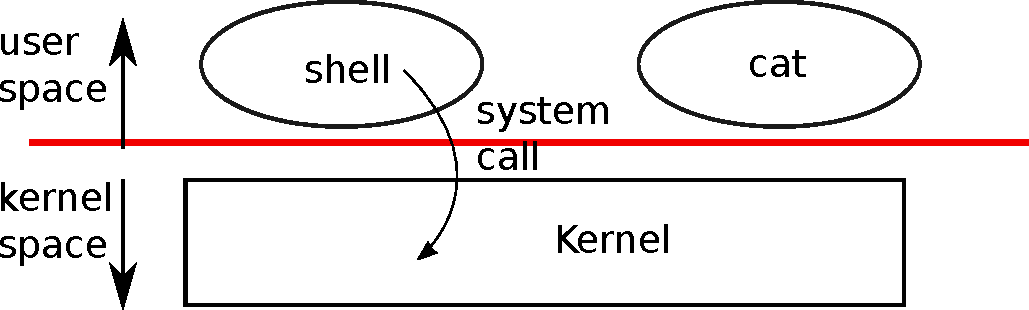
\includegraphics[scale=0.5]{fig/os.pdf}
\caption{一个内核和两个用户进程。  }
\label{fig:os}
\end{figure}     

内核提供的系统调用的集合是用户程序看到的接口。 xv6 内核提供了 Unix 内核传统上提供的服务和系统调用的子集。图~   \ref{fig:api}   列出了xv6的所有系统调用。  

本章的其余部分概述了 xv6 的服务——进程、内存、文件描述符、管道和文件系统——并用代码片段和讨论 Unix 的命令行用户界面    \indextext{shell}    如何使用它们来说明它们。 shell 对系统调用的使用说明了它们的设计是多么仔细。  

shell 是一个普通的程序,它读取用户的命令并执行它们。 shell 是一个用户程序,而不是内核的一部分,这一事实说明了系统调用接口的强大功能:shell 没有什么特别的。这也意味着外壳易于更换;因此,现代 Unix 系统有多种 shell 可供选择,每种都有自己的用户界面和脚本功能。 xv6 shell 是 Unix Bourne shell 本质的简单实现。它的实现可以在以下位置找到
    \lineref{user/sh.c:1}    。
    \section{进程和内存  }     

xv6 进程由用户空间内存(指令、数据和堆栈)和内核私有的每个进程状态组成。 Xv6
    \indextext{time-share}    进程:它在等待执行的进程集中透明地切换可用 CPU。当进程未执行时,xv6 会保存进程的 CPU 寄存器,并在下次运行进程时恢复它们。内核关联一个进程标识符,或者
    \indexcode{PID}    ,每个进程。  

   \begin{figure}[t]
\center
\begin{tabular}{ll}
{\bf System call} & {\bf Description}  \\ 
\midruleint fork() & Create a process, return child's PID.  \\ int exit(int status) & Terminate the current process; status reported to wait(). No return.  \\ int wait(int *status) & Wait for a child to exit; exit status in *status; returns child PID.  \\ int kill(int pid) & Terminate process PID. Returns 0, or -1 for error.  \\ int getpid() & Return the current process's PID.  \\ int sleep(int n) & Pause for n clock ticks.  \\ int exec(char *file, char *argv[]) & Load a file and execute it with arguments; only returns if error.  \\ char *sbrk(int n) & Grow process's memory by n bytes. Returns start of new memory.  \\ int open(char *file, int flags) & Open a file; flags indicate read/write; returns an fd (file descriptor).  \\ int write(int fd, char *buf, int n) & Write n bytes from buf to file descriptor fd; returns n.  \\ int read(int fd, char *buf, int n) & Read n bytes into buf; returns number read; or 0 if end of file.  \\ int close(int fd) & Release open file fd.  \\ int dup(int fd) & Return a new file descriptor referring to the same file as fd. \\ int pipe(int p[]) & Create a pipe, put read/write file descriptors in p[0] and p[1].  \\ int chdir(char *dir) & Change the current directory.  \\ int mkdir(char *dir) & Create a new directory.  \\ int mknod(char *file, int, int) & Create a device file.  \\ int fstat(int fd, struct stat *st) & Place info about an open file into *st.  \\ int stat(char *file, struct stat *st) & Place info about a named file into *st.  \\ int link(char *file1, char *file2) & Create another name (file2) for the file file1.  \\ int unlink(char *file) & Remove a file.  \\ 
\end{tabular}
\caption{Xv6 系统调用。如果没有另外说明,这些调用如果没有错误则返回 0,如果有错误则返回 -1。  }
\label{fig:api}
\end{figure}     

一个进程可以使用以下方法创建一个新进程
    \indexcode{fork}    系统调用。
    \lstinline{fork}    为新进程提供了调用进程内存的精确副本,包括指令和数据。
    \lstinline{fork}    在原始进程和新进程中均返回。在原始进程中,   \lstinline{fork}    返回新进程的 PID。在新进程中,   \lstinline{fork}    返回零。原始过程和新过程通常被称为
    \indextext{parent}    和
    \indextext{child}    。  

例如,考虑以下用 C 编程语言编写的程序片段~    \cite{kernighan}    :
    \begin{lstlisting}[]int pid = fork();if(pid > 0){
  printf("parent: child=
  pid = wait((int *) 0);
  printf("child 
} else if(pid == 0){
  printf("child: exiting\n");
  exit(0);
} else {
  printf("fork error\n");
}
\end{lstlisting}    该
    \indexcode{exit}    系统调用导致调用进程停止执行并释放内存和打开文件等资源。 Exit 采用整数状态参数,通常 0 表示成功,1 表示失败。这
    \indexcode{wait}    系统调用返回当前进程已退出(或已杀死)的子进程的 PID,并将子进程的退出状态复制到传递给 wait 的地址;如果调用者的孩子都没有退出,
    \indexcode{wait}    等待一个人这样做。如果调用者没有子项,   \lstinline{wait}    立即返回 -1。如果父进程不关心子进程的退出状态,它可以将 0 地址传递给
    \lstinline{wait}    。  

在示例中,输出行
    \begin{lstlisting}[]parent: child=1234child: exiting
\end{lstlisting}    可能以任一顺序出现(甚至混合),具体取决于父级或子级是否到达其
 首先调用    \indexcode{printf}   。孩子退出后,家长
    \indexcode{wait}    返回,导致父级打印
    \begin{lstlisting}[]parent: child 1234 is done
\end{lstlisting}    虽然子进程最初与父进程具有相同的内存内容,但父进程和子进程使用单独的内存和单独的寄存器执行:更改其中一个变量不会影响另一个变量。例如,当返回值为
    \lstinline{wait}    存储到
    \lstinline{pid}    在父进程中,它不会更改变量
 子项中的    \lstinline{pid}   。的价值
 子级中的    \lstinline{pid}    仍为零。  

这
    \indexcode{exec}    系统调用使用从文件系统中存储的文件加载的新内存映像替换调用进程的内存。该文件必须具有特定的格式,该格式指定文件的哪一部分保存指令、哪一部分是数据、从哪条指令开始等。Xv6 使用 ELF 格式,第    \ref{CH:MEM}    章对此进行了更详细的讨论。通常该文件是编译程序源代码的结果。什么时候
    \indexcode{exec}   成功,它不会返回到调用程序;而是从文件加载的指令在ELF头中声明的入口点开始执行。
    \lstinline{exec}    采用两个参数:包含可执行文件的文件名和字符串参数数组。例如:
    \begin{lstlisting}[]char *argv[3];

argv[0] = "echo";argv[1] = "hello";argv[2] = 0;exec("/bin/echo", argv);printf("exec error\n");
\end{lstlisting}    该片段用程序的实例替换调用程序
    \lstinline{/bin/echo}    使用参数列表运行
    \lstinline{echo}   
    \lstinline{hello}   。大多数程序都会忽略参数数组的第一个元素,它通常是程序的名称。  

xv6 shell 使用上述调用代表用户运行程序。外壳主要结构简单;看
    \lstinline{main}   
    \lineref{user/sh.c:/main/}    。主循环读取用户的一行输入
    \indexcode{getcmd}    。然后它调用
    \lstinline{fork}    ,它创建 shell 进程的副本。家长打电话
    \lstinline{wait}   ,当子进程运行命令时。例如,如果用户在 shell 中输入“   \lstinline{echo hello}   ”,
    \lstinline{runcmd}    将以“   \lstinline{echo hello}   ”作为参数进行调用。
    \lstinline{runcmd}   
    \lineref{user/sh.c:/runcmd/}    运行实际命令。对于“   \lstinline{echo hello}   ”,它将调用
    \lstinline{exec}   
    \lineref{user/sh.c:/exec.ecmd/}    。如果
    \lstinline{exec}    成功,那么子进程将执行来自
    \lstinline{echo}    而不是
    \lstinline{runcmd}    。在某一点
    \lstinline{echo}    将调用
    \lstinline{exit}    ,这将导致父级从
    \lstinline{wait}    中
    \lstinline{main}   
    \lineref{user/sh.c:/main/}    。  

你可能想知道为什么
    \indexcode{fork}    和
    \indexcode{exec}    未合并在一次调用中;稍后我们将看到 shell 在 I/O 重定向的实现中利用了分离。为了避免创建重复进程然后立即替换它(使用    \lstinline{exec}    )的浪费,操作内核优化了以下实现
 对于此用例,   \lstinline{fork}    使用虚拟内存技术,例如写入时复制(请参阅第    \ref{sec:pagefaults}    节)。  

Xv6 隐式分配大部分用户空间内存:
    \indexcode{fork}    分配父内存的子副本所需的内存,并且
    \indexcode{exec}    分配足够的内存来保存可执行文件。运行时需要更多内存的进程(可能是为了
    \indexcode{malloc}    )可以调用
    \lstinline{sbrk(n)}    将其数据内存增长
    \lstinline{n}    字节;
    \indexcode{sbrk}    返回新内存的位置。
    \section{I/O 和文件描述符  }     

A
    \indextext{file descriptor}    是一个小整数,表示进程可以读取或写入的内核管理对象。进程可以通过打开文件、目录或设备,或者通过创建管道,或者通过复制现有描述符来获取文件描述符。为了简单起见,我们经常将文件描述符所指的对象称为“文件”;文件描述符接口抽象出文件、管道和设备之间的差异,使它们看起来都像字节流。我们将输入和输出称为    \indextext{I/O}    。  

在内部,xv6 内核使用文件描述符作为每个进程表的索引,以便每个进程都有一个从零开始的文件描述符的私有空间。按照惯例,进程从文件描述符 0(标准输入)读取,将输出写入文件描述符 1(标准输出),并将错误消息写入文件描述符 2(标准错误)。正如我们将看到的,shell 利用该约定来实现 I/O 重定向和管道。 shell 确保它始终打开三个文件描述符
    \lineref{user/sh.c:/open..console/}    ,默认情况下是控制台的文件描述符。  

这
    \lstinline{read}    和
    \lstinline{write}    系统调用读取字节和写入字节以打开由文件描述符命名的文件。电话
    \lstinline{read(fd}    ,
    \lstinline{buf}    ,
    \lstinline{n)}    最多读取
 文件描述符中的    \lstinline{n}    字节
    \lstinline{fd}    ,将它们复制到
    \lstinline{buf}    ,并返回读取的字节数。引用文件的每个文件描述符都有一个与其关联的偏移量。
    \lstinline{read}    从当前文件偏移量读取数据,然后将偏移量前进读取的字节数:后续
    \lstinline{read}    将返回第一个返回的字节之后的字节
    \lstinline{read}    。当没有更多字节可读取时,
    \lstinline{read}    返回零以指示文件结尾。  

电话
    \lstinline{write(fd}    ,
    \lstinline{buf}    ,
    \lstinline{n)}    写入
    \lstinline{n}    字节来自
    \lstinline{buf}    到文件描述符
    \lstinline{fd}    并返回写入的字节数。少于
 仅当发生错误时才会写入    \lstinline{n}    字节。喜欢
    \lstinline{read}    ,
    \lstinline{write}    在当前文件偏移处写入数据,然后将该偏移量前进写入的字节数:每个
    \lstinline{write}    从上一个停止的地方继续。  

下面的程序片段(构成了程序的本质)
    \lstinline{cat}    )将数据从其标准输入复制到其标准输出。如果发生错误,它将向标准错误写入一条消息。
    \begin{lstlisting}[]char buf[512];int n;

for(;;){
  n = read(0, buf, sizeof buf);
  if(n == 0)
    break;
  if(n < 0){
    fprintf(2, "read error\n");
    exit(1);
  }
  if(write(1, buf, n) != n){
    fprintf(2, "write error\n");
    exit(1);
  }
}
\end{lstlisting}    代码片段中需要注意的重要一点是
    \lstinline{cat}    不知道它是从文件、控制台还是管道读取。相似地
    \lstinline{cat}    不知道它是否正在打印到控制台、文件或其他什么。文件描述符的使用以及文件描述符 0 作为输入、文件描述符 1 作为输出的约定允许简单地实现
    \lstinline{cat}    。  

这
    \lstinline{close}    系统调用释放文件描述符,使其可供将来重用
    \lstinline{open}    ,
    \lstinline{pipe}   ,或
    \lstinline{dup}    系统调用(见下文)。新分配的文件描述符始终是当前进程中编号最小的未使用描述符。  

文件描述符和
    \indexcode{fork}    交互使 I/O 重定向易于实现。
    \lstinline{fork}    复制父级的文件描述符表及其内存,以便子级以与父级完全相同的打开文件开始。系统调用
    \indexcode{exec}    替换调用进程的内存,但保留其文件表。此行为允许 shell 通过分叉、重新打开子级中选定的文件描述符,然后调用    \lstinline{exec}    来运行新程序来实现    \indextext{I/O redirection}   。这是 shell 为命令运行的代码的简化版本
    \lstinline{cat}   
    \lstinline{<}   
    \lstinline{input.txt}   :
    \begin{lstlisting}[]char *argv[2];

argv[0] = "cat";argv[1] = 0;if(fork() == 0) {
  close(0);
  open("input.txt", O_RDONLY);
  exec("cat", argv);
}
\end{lstlisting}    子进程关闭文件描述符0后,
    \lstinline{open}    保证为新打开的文件使用该文件描述符
    \lstinline{input.txt}    :0 将是最小的可用文件描述符。
    \lstinline{cat}    然后使用文件描述符 0(标准输入)执行,引用
    \lstinline{input.txt}    。此序列不会更改父进程的文件描述符,因为它仅修改子进程的描述符。  

xv6 shell 中 I/O 重定向的代码正是以这种方式工作的
    \lineref{user/sh.c:/case.REDIR/}    。回想一下,此时在代码中,shell 已经分叉了子 shell,并且
    \lstinline{runcmd}    将调用
    \lstinline{exec}    加载新程序。  

   \lstinline{open}    的第二个参数包含一组关闭标志(以位表示),用于控制    \lstinline{open}    的操作。可能的值在文件控制 (fcntl) 标头中定义
    \linerefs{kernel/fcntl.h:/RDONLY/,/TRUNC/}   :
    \lstinline{O_RDONLY}    ,
    \lstinline{O_WRONLY}    ,
    \lstinline{O_RDWR}    ,
    \lstinline{O_CREATE}    和
    \lstinline{O_TRUNC}    ,指示    \lstinline{open}    打开文件进行读取、或写入、或读取和写入,如果文件不存在则创建文件,并将文件截断为零长度。  

现在应该清楚为什么它有帮助了
    \lstinline{fork}    和
    \lstinline{exec}    是单独的调用:在两者之间,shell 有机会重定向子 shell 的 I/O,而不会干扰主 shell 的 I/O 设置。人们可以想象一种假设的组合
    \lstinline{forkexec}    系统调用,但使用此类调用进行 I/O 重定向的选项似乎很尴尬。 shell 可以在调用    \lstinline{forkexec}    之前修改自己的 I/Osetup(然后取消这些修改);或者
    \lstinline{forkexec}    可以将 I/O 重定向指令作为参数;或者(最不吸引人的)每个像    \lstinline{cat}    这样的程序都可以被教导执行自己的 I/O 重定向。  

虽然
    \lstinline{fork}    复制文件描述符表,每个底层文件偏移量在父级和子级之间共享。考虑这个例子:
    \begin{lstlisting}[]if(fork() == 0) {
  write(1, "hello ", 6);
  exit(0);
} else {
  wait(0);
  write(1, "world\n", 6);
}
\end{lstlisting}    在此片段的末尾,附加到文件描述符 1 的文件将包含数据
    \lstinline{hello}   
    \lstinline{world}    。这
 父级中的    \lstinline{write}    (这要归功于
    \lstinline{wait}   ,仅在子进程完成后运行)拾取子进程的位置
    \lstinline{write}    已停止。此行为有助于从 shell 命令序列中生成顺序输出,例如
    \lstinline{(echo}   
    \lstinline{hello}   ;
    \lstinline{echo}   
    \lstinline{world)}   
    \lstinline{>output.txt}    。  

这
    \lstinline{dup}    系统调用复制现有文件描述符,返回引用同一底层 I/O 对象的新文件描述符。两个文件描述符共享一个偏移量,就像文件描述符复制一样
    \lstinline{fork}    做。这是另一种写法
    \lstinline{hello}   
    \lstinline{world}    到文件中:
    \begin{lstlisting}[]fd = dup(1);write(1, "hello ", 6);write(fd, "world\n", 6);
\end{lstlisting}     

如果两个文件描述符是通过一系列从同一个原始文件描述符派生而来的,则它们共享一个偏移量
    \lstinline{fork}    和
    \lstinline{dup}    调用。否则文件描述符不共享偏移量,即使它们是由
    \lstinline{open}    调用相同的文件。
    \lstinline{dup}    允许 shell 实现如下命令:
    \lstinline{ls}   
    \lstinline{existing-file}   
    \lstinline{non-existing-file}   
    \lstinline{>}   
    \lstinline{tmp1}   
    \lstinline{2>&1}    。这
    \lstinline{2>&1}    告诉 shell 为命令提供一个文件描述符 2,它是描述符 1 的副本。现有文件的名称和不存在文件的错误消息都将显示在文件中
    \lstinline{tmp1}    。 xv6 shell 不支持错误文件描述符的 I/O 重定向,但现在您知道如何实现它。  

文件描述符是一个强大的抽象,因为它们隐藏了它们所连接的内容的详细信息:写入文件描述符 1 的进程可能正在写入文件、控制台等设备或管道。
    \section{管道  }     

A
    \indextext{pipe}    是一个小型内核缓冲区,作为一对文件描述符向进程公开,一个用于读取,一个用于写入。将数据写入管道的一端使得该数据可用于从管道的另一端读取。管道为进程提供了一种通信方式。  

下面的示例代码运行程序
    \lstinline{wc}    具有连接到管道读取端的标准输入。
    \begin{lstlisting}[]int p[2];char *argv[2];

argv[0] = "wc";argv[1] = 0;

pipe(p);if(fork() == 0) {
  close(0);
  dup(p[0]);
  close(p[0]);
  close(p[1]);
  exec("/bin/wc", argv);
} else {
  close(p[0]);
  write(p[1], "hello world\n", 12);
  close(p[1]);
}
\end{lstlisting}    程序调用
    \lstinline{pipe}    ,创建一个新管道并将读写文件描述符记录在数组中
    \lstinline{p}    。后
    \lstinline{fork}    ,父级和子级都有引用管道的文件描述符。子进程调用   \lstinline{close}   和   \lstinline{dup}   使文件描述符zero指向管道的读取端,关闭文件描述符
    \lstinline{p}    ,并调用   \lstinline{exec}   运行
    \lstinline{wc}    。什么时候
    \lstinline{wc}    从其标准输入读取,从管道读取。父级关闭管道的读取端,写入管道,然后关闭写入端。  

如果没有可用数据,则
 管道上的    \lstinline{read}    等待数据写入或引用写入端的所有文件描述符关闭;在后一种情况下,
    \lstinline{read}    将返回 0,就像已到达数据文件末尾一样。事实是
    \lstinline{read}    会阻塞,直到新数据不可能到达为止,这是子进程在执行之前关闭管道的写入端很重要的原因之一
 上面的    \lstinline{wc}   :如果其中之一
    \lstinline{wc}    的文件描述符引用管道的写入端,
    \lstinline{wc}    永远不会看到文件结尾。  

xv6 shell 实现了诸如
    \lstinline{grep fork sh.c | wc -l}    的方式与上面的代码类似
    \lineref{user/sh.c:/case.PIPE/}    。子进程创建一个管道来连接管道的左端和右端。然后它调用
    \lstinline{fork}    和
    \lstinline{runcmd}    表示管道的左端
    \lstinline{fork}    和
    \lstinline{runcmd}    为右端,并等待两者完成。管道的右端可能是本身包含 apipe 的命令(例如,
    \lstinline{a}   
    \lstinline{|}   
    \lstinline{b}   
    \lstinline{|}   
    \lstinline{c)}    ,它本身分叉两个新的子进程(一个用于
    \lstinline{b}    和一个用于
    \lstinline{c}    )。因此,shell 可以创建进程树。这棵树的叶子是命令,内部节点是等待左右子节点完成的进程。  

管道可能看起来并不比临时文件更强大:管道
    \begin{lstlisting}[]echo hello world | wc
\end{lstlisting}    可以在没有管道的情况下实现,如下所示
 在这种情况下,   \begin{lstlisting}[]echo hello world >/tmp/xyz; wc </tmp/xyz
\end{lstlisting}    管道比临时文件至少具有三个优点。首先,管道会自动清理自身;通过文件重定向,shell 必须小心地删除
 完成后    \lstinline{/tmp/xyz}   。其次,管道可以传递任意长的数据流,而文件重定向需要磁盘上有足够的可用空间来存储所有数据。第三,管道允许并行执行管道阶段,而文件方法要求第一个程序在第二个程序开始之前完成。
    \section{文件系统  }     

xv6 文件系统提供数据文件(包含未解释的字节数组)和目录(包含对数据文件和其他目录的命名引用)。这些目录形成一棵树,从一个称为
    \indextext{root}    。 A
    \indextext{path}    喜欢
    \lstinline{/a/b/c}    指的是名为的文件或目录
    \lstinline{c}    位于名为的目录中
    \lstinline{b}    位于名为的目录中
 根目录中的    \lstinline{a}   
    \lstinline{/}   。不以以下方式开头的路径
    \lstinline{/}    是相对于调用进程的进行评估的
    \indextext{current directory}    ,可以使用以下命令更改
    \lstinline{chdir}    系统调用。这两个代码片段都打开同一个文件(假设所有涉及的目录都存在):
    \begin{lstlisting}[]chdir("/a");chdir("b");open("c", O_RDONLY);

open("/a/b/c", O_RDONLY);
\end{lstlisting}    第一个片段将进程的当前目录更改为
    \lstinline{/a/b}    ;第二个既不引用也不更改进程的当前目录。  

有系统调用来创建新文件和目录:
    \lstinline{mkdir}    创建一个新目录,
    \lstinline{open}    与
    \lstinline{O_CREATE}    标志创建一个新的数据文件,并且
    \lstinline{mknod}    创建一个新的设备文件。此示例说明了所有三个:
    \begin{lstlisting}[]mkdir("/dir");fd = open("/dir/file", O_CREATE|O_WRONLY);close(fd);mknod("/console", 1, 1);
\end{lstlisting}   
    \lstinline{mknod}    创建一个引用设备的特殊文件。与设备文件关联的是主设备号和次设备号(这两个参数
    \lstinline{mknod}    ),唯一标识一个内核设备。当进程稍后打开设备文件时,内核会转移
    \lstinline{read}    和
    \lstinline{write}    系统调用内核设备实现,而不是将它们传递到文件系统。  

文件名与文件本身不同;相同的底层文件,称为
    \indextext{inode}    ,可以有多个名称,称为
    \indextext{links}    。每个链接由目录中的一个条目组成;该条目包含文件名和对索引节点的引用。一个 inode 保存
    \indextext{metadata}    关于文件,包括其类型(文件或目录或设备)、其长度、文件内容在磁盘上的位置以及文件的链接数。  

这
    \lstinline{fstat}    系统调用从文件描述符引用的索引节点检索信息。它填写一个
    \lstinline{struct}   
    \lstinline{stat}    ,定义于
    \lstinline{stat.h}       \fileref{kernel/stat.h}    为:
    \begin{lstlisting}[]
#define T_DIR     1   // Directory
#define T_FILE    2   // File
#define T_DEVICE  3   // Device

struct stat {
  int dev;     // File system's disk device
  uint ino;    // Inode number
  short type;  // Type of file
  short nlink; // Number of links to file
  uint64 size; // Size of file in bytes
};
\end{lstlisting}     

这
    \lstinline{link}    系统调用创建另一个文件系统名称,引用与现有文件相同的 inode。该片段创建一个名为both 的新文件
    \lstinline{a}    和
    \lstinline{b}    。
    \begin{lstlisting}[]open("a", O_CREATE|O_WRONLY);link("a", "b");
\end{lstlisting}    读取或写入
    \lstinline{a}    与读取或写入相同
    \lstinline{b}    。每个索引节点都由唯一的索引节点号标识。经过上面的代码序列,可以确定
    \lstinline{a}    和
    \lstinline{b}    通过检查结果来引用相同的底层内容
    \lstinline{fstat}    :两者都会返回相同的索引节点号(    \lstinline{ino}    ),并且
    \lstinline{nlink}    计数将设置为 2。  

这
    \lstinline{unlink}    系统调用从文件系统中删除名称。仅当文件的链接计数为零并且没有文件描述符引用它时,文件的索引节点和保存其内容的磁盘空间才会被释放。因此添加
    \begin{lstlisting}[]unlink("a");
\end{lstlisting}    到最后一个代码序列使 inode 和文件内容可访问为
    \lstinline{b}    。此外,
    \begin{lstlisting}[]fd = open("/tmp/xyz", O_CREATE|O_RDWR);unlink("/tmp/xyz");
\end{lstlisting}    是创建没有名称的临时索引节点的惯用方法,该索引节点将在进程关闭时被清理
    \lstinline{fd}    或退出。  

Unix 提供了可从 shellas 用户级程序调用的文件实用程序,例如
    \lstinline{mkdir}    ,
    \lstinline{ln}    和
    \lstinline{rm}    。这种设计允许任何人通过添加新的用户级程序来扩展命令行界面。事后看来,这个计划似乎是显而易见的,但 Unix 时代设计的其他系统经常将此类命令内置到 shell 中(并将 shell 内置到内核中)。  

一个例外是
    \lstinline{cd}    ,内置于 shell 中
    \lineref{user/sh.c:/if.buf.0..==..c./}    。
    \lstinline{cd}    必须更改 shell 本身的当前工作目录。如果
    \lstinline{cd}    作为常规命令运行,然后 shell 会分叉一个子进程,子进程将运行
    \lstinline{cd}    和
    \lstinline{cd}    将更改子进程的工作目录。父级(即 shell 的)工作目录不会更改。
    \section{真实世界  }     

Unix 将“标准”文件描述符、管道和对其进行操作的方便的 shell 语法相结合,这是编写通用可重用程序的一大进步。这个想法引发了一种“软件工具”文化,这种文化对 Unix 的强大和普及负有重要责任,而 shell 是第一个所谓的“脚本语言”。Unix 系统调用接口至今仍然存在于 BSD 等系统中, Linux 和 macOS。  

Unix 系统调用接口已通过可移植操作系统接口 (POSIX) 标准进行了标准化。 Xv6 不符合 POSIX:它缺少许多系统调用(包括基本的系统调用,例如
    \lstinline{lseek}    ),并且它提供的许多系统调用与标准不同。我们 xv6 的主要目标是简单和清晰,同时提供简单的类 UNIX 系统调用接口。有几个人用更多的系统调用和简单的 C 库扩展了 xv6,以便运行基本的 Unix 程序。然而,现代内核比 xv6 提供更多的系统调用和更多种类的内核服务。例如,它们支持网络、窗口系统、用户级线程、许多设备的驱动程序等等。现代内核不断快速发展,并提供了许多超越 POSIX 的功能。  

Unix 通过一组文件名和文件描述符接口统一访问多种类型的资源(文件、目录和设备)。这个想法可以扩展到更多种类的资源;一个很好的例子是 Plan 9~    \cite{Presotto91plan9}    ,它将“资源就是文件”的概念应用于网络、图形等。然而,大多数 Unix 派生的操作系统并没有遵循这条路线。  

文件系统和文件描述符是强大的抽象。即便如此,操作系统接口还有其他模型。 Multics 是 Unix 的前身,它以一种看起来像内存的方式抽象文件存储,从而产生了一种截然不同的界面风格。 Multics 设计的复杂性对 Unix 的设计者产生了直接影响,他们的目标是构建更简单的东西。  

Xv6 不提供用户或保护一个用户免受另一个用户侵害的概念;在 Unix 术语中,所有 xv6 进程都以 root 身份运行。  

本书探讨了 xv6 如何实现其类 Unix 接口,但其中的思想和概念不仅仅适用于 Unix。任何操作系统都必须将进程复用到底层硬件上,将进程彼此隔离,并提供受控进程间通信的机制。研究完 xv6 后,您应该能够了解其他更复杂的操作系统,并了解这些系统中 xv6 的基本概念。
    \section{练习  }     

   \begin{enumerate}


   \item   编写一个程序,使用 UNIX 系统调用通过一对管道(每个方向一个)在两个进程之间“乒乓”一个字节。衡量程序的性能,以每秒的交换次数为单位。  \end{enumerate}     

\end{document}

   
    
\documentclass[UTF8]{article}
\usepackage{xeCJK}
\usepackage{amsmath,amssymb}
\begin{document}


  

   \chapter{Operating system organization}   
    \label{CH:FIRST}     

操作系统的一个关键要求是同时支持多个活动。例如,使用 Chapter~    \ref{CH:UNIX}    中描述的系统调用接口,进程可以启动新进程:
    \lstinline{fork}    。操作系统必须
    \indextext{time-share}    这些进程中的计算机资源。例如,即使进程数量多于硬件 CPU 数量,操作系统也必须确保所有进程都有机会执行。操作系统还必须安排
 进程之间的    \indextext{isolation}   。也就是说,如果一个进程有错误并且发生故障,它不应该影响不依赖于有错误的进程的进程。然而,完全隔离太强了,因为进程应该可以有意地交互;管道就是一个例子。因此操作系统必须满足三个要求:复用、隔离和交互。  

本章概述了如何组织操作系统来实现这三个要求。事实证明,有很多方法可以做到这一点,但本文重点关注以    \indextext{monolithic kernel}    为中心的主流设计,许多 Unix 操作系统都使用它。本章还概述了 xv6 进程(xv6 中的隔离单元),以及 xv6 启动时第一个进程的创建。  

Xv6 在    \indextext{multi-core}       \footnote{本文中的“多核”是指共享内存但并行执行的多个 CPU,每个 CPU 都有自己的一组寄存器。本文有时使用术语
    \indextext{multiprocessor}    是多核的同义词,但多处理器也可以更具体地指具有多个不同处理器芯片的计算机。  }    RISC-V 微处理器上运行,其许多低级功能(例如,其流程实现)特定于 RISC-V。 RISC-V是64位CPU,xv6是用“LP64”C编写的,这意味着C编程语言中的long(L)和指针(P)是64位,但int是32位。本书假设读者已经在某些架构上完成了一些机器级编程,并将在出现时介绍 RISC-V 特定的想法。 RISC-V 的有用参考是“RISC-V 阅读器:开放架构图集”~    \cite{riscv}   。用户级 ISA~    \cite{riscv:user}    和特权架构~    \cite{riscv:priv}    是官方规范。  

完整计算机中的 CPU 周围环绕着支持硬件,其中大部分以 I/O 接口的形式存在。 Xv6 是为 qemu 的“-machine virt”选项模拟的支持硬件而编写的。这包括 RAM、包含启动代码的 ROM、与用户键盘/屏幕的串行连接以及用于存储的磁盘。
    \section{抽象物理资源  }     

当遇到操作系统时,人们可能会问的第一个问题是为什么要有它?也就是说,可以将图 ~    \ref{fig:api}    中的系统调用实现为一个库,应用程序可以与该库链接。在这个计划中,每个应用程序甚至可以拥有自己的适合其需求的库。应用程序可以直接与硬件资源交互,并以最适合应用程序的方式使用这些资源(例如,实现高或可预测的性能)。一些嵌入式设备或实时系统的操作系统就是以这种方式组织的。  

这种库方法的缺点是,如果有多个应用程序正在运行,则这些应用程序必须表现良好。例如,每个应用程序必须定期放弃CPU,以便其他应用程序可以运行。如果所有应用程序相互信任并且没有错误,那么这种协作分时方案可能是可行的。对于应用程序来说,更常见的是彼此不信任并且存在错误,因此人们通常需要比协作方案提供的更强的隔离。  

为了实现强隔离,禁止应用程序直接访问敏感硬件资源,并将资源抽象为服务,会很有帮助。例如,Unix 应用程序仅通过文件系统的
    \lstinline{open}    ,
    \lstinline{read}    ,
    \lstinline{write}    和
    \lstinline{close}   系统调用,而不是直接读写磁盘。这为应用程序提供了路径名的便利,并且允许操作系统(作为接口的实现者)管理磁盘。即使隔离不是一个问题,有意交互(或只是希望不妨碍彼此)的程序也可能会发现文件系统是比直接使用磁盘更方便的抽象。  

类似地,Unix在进程之间透明地切换硬件CPU,根据需要保存和恢复寄存器状态,这样应用程序就不必担心时间共享。即使某些应用程序处于无限循环中,这种透明度也允许操作系统共享 CPU。  

另一个例子,Unix 进程使用
    \lstinline{exec}    来构建它们的内存映像,而不是直接与物理内存交互。这允许操作系统决定将进程放置在内存中的位置;如果内存紧张,操作系统甚至可能将某些进程的数据存储在磁盘上。
    \lstinline{exec}   还为用户提供了方便的文件系统来存储可执行程序映像。  

Unix 进程之间的许多交互形式都是通过文件描述符发生的。文件描述符不仅抽象了许多细节(例如,管道或文件中的数据存储位置),而且还以简化交互的方式进行定义。例如,如果管道中的一个应用程序失败,内核将为管道中的下一个进程生成文件结束信号。  

图~   \ref{fig:api}   中的系统调用接口经过精心设计,既为程序员提供了便利,又提供了强隔离的可能性。 Unix 接口并不是抽象资源的唯一方法,但它已被证明是一个非常好的方法。
    \section{用户模式、管理员模式和系统调用  }     

强隔离需要应用程序和操作系统之间有硬边界。如果应用程序出错,我们不希望操作系统失败或其他应用程序失败。相反,操作系统应该能够清理失败的应用程序并继续运行其他应用程序。为了实现强隔离,操作系统必须安排应用程序不能修改(甚至读取)操作系统的数据结构和指令,并且应用程序不能访问其他进程的内存。  

CPU为强隔离提供硬件支持。例如,RISC-V具有三种CPU执行指令的模式:
    \indextext{machine mode}    ,
    \indextext{supervisor mode}    和
    \indextext{user mode}    。在机器模式下执行的指令具有完全特权; CPU 以机器模式启动。机器模式主要用于配置计算机。 Xv6 在机器模式下执行几行,然后更改为管理模式。  

在管理模式下,CPU 可以执行
    \indextext{privileged instructions}    :例如,启用和禁用中断、读取和写入保存页表地址的寄存器等。如果用户模式下的应用程序尝试执行特权指令,则CPU不会执行该指令,而是切换到管理程序模式,以便主管模式代码可以终止应用程序,因为它做了一些不应该做的事情。第〜   \ref{CH:UNIX}   中的图〜   \ref{fig:os}   说明了这种组织。应用程序只能执行用户模式指令(例如,添加数字等),并且据说运行在
    \indextext{user space}   ,而管理模式下的软件也可以执行特权指令,据说运行在
    \indextext{kernel space}    。运行在内核空间(或管理模式)的软件称为
    \indextext{kernel}    。  

想要调用内核函数的应用程序(例如
 xv6 中的    \lstinline{read}    系统调用必须转换到内核;应用程序不能直接调用内核函数。 CPU 提供了一种特殊的指令,可以将 CPU 从用户模式切换到管理模式,并在内核指定的入口点进入内核。 (RISC-V 提供
    \indexcode{ecall}    指令用于此目的。)一旦 CPU 切换到管理模式,内核就可以验证系统调用的参数(例如,检查传递给系统调用的地址是否是应用程序内存的一部分),决定应用程序是否允许执行请求的操作(例如,检查应用程序是否允许写入指定的文件),然后拒绝或执行它。内核控制转换到管理模式的入口点非常重要;例如,如果应用程序可以决定内核入口点,则恶意应用程序可以在跳过参数验证的点进入内核。
    \section{内核组织  }     

一个关键的设计问题是操作系统的哪一部分应该在管理模式下运行。一种可能性是整个操作系统驻留在内核中,以便所有系统调用的实现都在管理程序模式下运行。这个组织被称为
    \indextext{monolithic kernel}    。  

在这个组织中,整个操作系统以完全的硬件权限运行。这种组织很方便,因为操作系统设计者不必决定操作系统的哪一部分不需要完整的硬件权限。此外,操作系统的不同部分更容易协作。例如,操作系统可能具有可由文件系统和虚拟内存系统共享的缓冲区高速缓存。  

整体组织的缺点是操作系统不同部分之间的接口通常很复杂(正如我们将在本文的其余部分中看到的),因此操作系统开发人员很容易犯错误。在单片内核中,错误是致命的,因为管理模式下的错误通常会导致内核失败。如果内核出现故障,计算机就会停止工作,因此所有应用程序也会失败。计算机必须重新启动才能重新启动。  

为了降低内核出错的风险,操作系统设计者可以最大限度地减少在管理模式下运行的操作系统代码量,并在用户模式下执行操作系统的大部分代码。这个内核组织称为
    \indextext{microkernel}    。  

   \begin{figure}[t]
\center
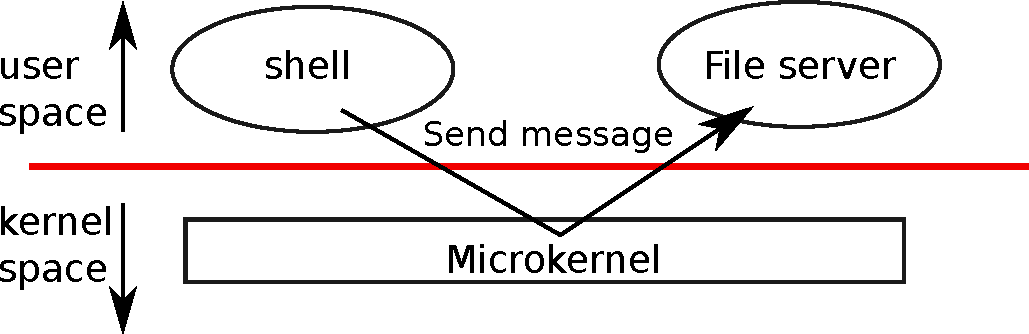
\includegraphics[scale=0.5]{fig/mkernel.pdf}
\caption{带有文件系统服务器的微内核  }
\label{fig:mkernel}
\end{figure}     

图~    \ref{fig:mkernel}    说明了这种微内核设计。在图中,文件系统作为用户级进程运行。作为进程运行的操作系统服务称为服务器。为了允许应用程序与文件服务器交互,内核提供了进程间通信机制,将消息从一个用户模式进程发送到另一个用户模式进程。例如,如果像 shell 这样的应用程序想要读取或写入文件,它会向文件服务器发送一条消息并等待响应。  

在微内核中,内核接口由一些低级函数组成,用于启动应用程序、发送消息、访问设备硬件等。这种组织使内核相对简单,因为大多数操作系统驻留在用户级服务器中。  

在现实世界中,整体内核和微内核都很流行。许多 Unix 内核都是单一的。例如,Linux 具有整体内核,尽管某些操作系统功能作为用户级服务器运行(例如窗口系统)。 Linux 为操作系统密集型应用程序提供了高性能,部分原因是内核的子系统可以紧密集成。  

Minix、L4 和 QNX 等操作系统被组织为带有服务器的微内核,并且在嵌入式设置中得到了广泛部署。 L4 的变体 seL4 足够小,已经过内存安全和其他安全属性的验证~    \cite{sel4}    。  

关于哪个组织更好,操作系统开发人员之间存在很多争论,并且没有任何确凿的证据。此外,它很大程度上取决于“更好”的含义:更快的性能、更小的代码大小、内核的可靠性、整个操作系统的可靠性(包括用户级服务)等。  

还有一些实际考虑因素可能比哪个组织的问题更重要。一些操作系统具有微内核,但出于性能原因在内核空间中运行一些用户级服务。一些操作系统具有整体内核,因为它们就是这样开始的,并且几乎没有动力转向纯粹的微内核组织,因为新功能可能比重写现有操作系统以适应微内核设计更重要。  

从本书的角度来看,微内核和单片操作系统有许多共同的关键思想。它们实现系统调用、使用页表、处理中断、支持进程、使用锁进行并发控制、实现文件系统等。本书重点讨论这些核心思想。  

与大多数 Unix 操作系统一样,Xv6 是作为整体内核实现的。由此可见,xv6内核接口对应于操作系统接口,内核实现了完整的操作系统。由于 xv6 不提供很多服务,因此它的内核比某些微内核要小,但从概念上讲 xv6 是整体的。  

   \section{代码:xv6 组织  }     

   \begin{figure}[t]
\center
\begin{tabular}{l|l}
{\bf File} & {\bf Description}  \\ 
\midrulebio.c & Disk block cache for the file system.  \\ console.c & Connect to the user keyboard and screen.  \\ entry.S & Very first boot instructions.  \\ exec.c & exec() system call.  \\ file.c & File descriptor support.  \\ fs.c & File system.  \\ kalloc.c & Physical page allocator.  \\ kernelvec.S & Handle traps from kernel, and timer interrupts.  \\ log.c & File system logging and crash recovery.  \\ main.c & Control initialization of other modules during boot.  \\ pipe.c & Pipes.  \\ plic.c & RISC-V interrupt controller.  \\ printf.c & Formatted output to the console.  \\ proc.c & Processes and scheduling.  \\ sleeplock.c & Locks that yield the CPU.  \\ spinlock.c & Locks that don't yield the CPU.  \\ start.c & Early machine-mode boot code.  \\ string.c & C string and byte-array library.  \\ swtch.S & Thread switching.  \\ syscall.c & Dispatch system calls to handling function.  \\ sysfile.c & File-related system calls.  \\ sysproc.c & Process-related system calls.  \\ trampoline.S & Assembly code to switch between user and kernel.  \\ trap.c & C code to handle and return from traps and interrupts.  \\ uart.c & Serial-port console device driver.  \\ virtio\_disk.c & Disk device driver.  \\ vm.c & Manage page tables and address spaces.  \\ 
\end{tabular}
\caption{Xv6 内核源文件。  }
\label{fig:source}
\end{figure}     

xv6 内核源代码位于  {    \tt   内核/   }  子目录中。源代码被分成文件,遵循模块化的粗略概念;图~    \ref{fig:source}    列出了这些文件。模块间接口在    \lstinline{defs.h}       \fileref{kernel/defs.h}    中定义。
    \section{流程概览  }     

xv6 中的隔离单位(与其他 Unix 操作系统一样)是
    \indextext{process}    。进程抽象可以防止一个进程破坏或监视另一个进程的内存、CPU、文件描述符等。它还可以防止进程破坏内核本身,因此进程无法破坏内核的隔离机制。内核必须小心地实现进程抽象,因为有错误或恶意的应用程序可能会欺骗内核或硬件做一些坏事(例如,规避隔离)。内核用来实现进程的机制包括用户/管理程序模式标志、地址空间和线程的时间分片。  

为了帮助实施隔离,进程抽象为程序提供了它拥有自己的私有机器的错觉。进程为程序提供了看似私有的内存系统,或者
    \indextext{address space}    ,其他进程无法读取或写入。进程还为程序提供看似其自己的 CPU 来执行程序的指令。  

Xv6 使用页表(由硬件实现)为每个进程提供自己的地址空间。 RISC-V 页表转换(或“映射”)a
    \indextext{virtual address}   (RISC-V 指令操作的地址)到
    \indextext{physical address}   (CPU芯片发送到主存的地址)。  

   \begin{figure}[t]
\centering
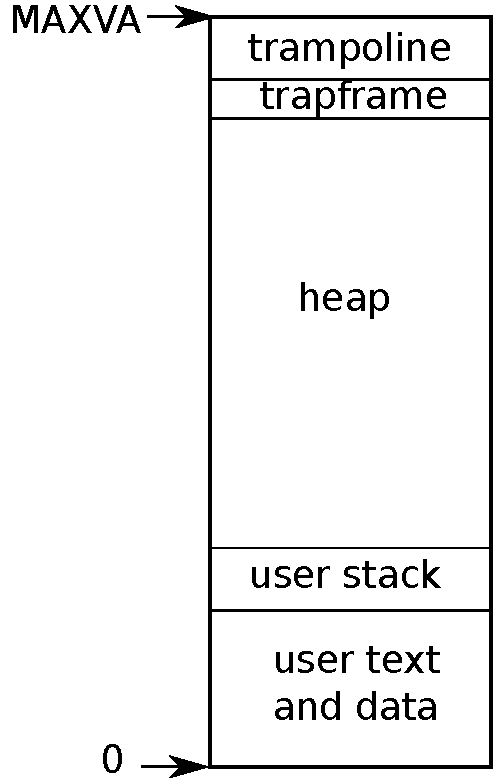
\includegraphics[scale=0.5]{fig/as.pdf}
\caption{进程虚拟地址空间的布局  }
\label{fig:as}
\end{figure}     

Xv6 为每个进程维护一个单独的页表,用于定义该进程的地址空间。如图~   \ref{fig:as}   所示,地址空间包括进程的
    \indextext{user memory}    从虚拟地址零开始。首先是指令,然后是全局变量,然后是堆栈,最后是进程可以根据需要扩展的“堆”区域(用于 malloc)。有很多因素限制了进程地址空间的最大大小:RISC-V 上的指针是 64 位宽;硬件在页表中查找虚拟地址时仅使用低 39 位;而 xv6 仅使用其中的 38 位39 位。因此,最大地址为    $2^{38}-1$    = 0x3fffffffff,即    \lstinline{MAXVA}    ~    \lineref{kernel/riscv.h:/define.MAXVA/}    。在地址空间的顶部,xv6 保留一个用于    \indextext{trampoline}    的页面和一个映射进程的    \indextext{trapframe}    的页面。 Xv6 使用这两个页面来转换到内核并返回;trampoline 页包含转换进和出内核的代码,并且映射 trapframe 对于保存/恢复用户进程的状态是必要的,正如我们将在第    \ref{CH:TRAP}    章中解释的那样。  

xv6 内核为每个进程维护许多状态,并将其收集到一个
    \indexcode{struct proc}   
    \lineref{kernel/proc.h:/^struct.proc/}    。进程最重要的内核状态部分是其页表、内核堆栈和运行状态。我们将使用符号
    \indexcode{p->xxx}    引用的元素
    \lstinline{proc}   结构;例如,
    \indexcode{p->pagetable}    是指向进程页表的指针。  

每个进程都有一个执行线程(或
    \indextext{thread}   (简称   \indextext{thread}   )执行进程的指令。线程可以挂起并稍后恢复。为了在进程之间透明地切换,内核挂起当前正在运行的线程并恢复另一个进程的线程。线程的大部分状态(局部变量、函数调用返回地址)都存储在线程的堆栈中。每个进程都有两个堆栈:用户堆栈和内核堆栈 (    \indexcode{p->kstack}    )。当进程执行用户指令时,只有用户堆栈在使用,而内核堆栈为空。当进程进入内核时(进行系统调用或中断),内核代码在进程的内核堆栈上执行;当进程位于内核中时,其用户堆栈仍然包含保存的数据,但没有被主动使用。进程的线程在主动使用其用户堆栈和其内核堆栈之间交替。内核堆栈是独立的(并受到用户代码的保护),因此即使进程破坏了其用户堆栈,内核也可以执行。  

进程可以通过执行 RISC-V    \indexcode{ecall}    指令来进行系统调用。该指令提高了硬件特权级别并将程序计数器更改为内核定义的入口点。入口点的代码切换到内核堆栈并执行实现系统调用的内核指令。当系统调用完成后,内核通过调用   \indexcode{sret}   指令切换回用户堆栈并返回用户空间,这会降低硬件权限级别并在系统调用指令之后恢复执行用户指令。进程的线程可以在内核中“阻塞”以等待 I/O,并在 I/O 完成时从中断处恢复。  

   \indexcode{p->state}    指示进程是否已分配、准备运行、正在运行、正在等待 I/O 或正在退出。  

   \indexcode{p->pagetable}    以 RISC-V 硬件期望的格式保存进程的页表。 Xv6 导致分页硬件使用进程的
 在用户空间中执行该进程时    \lstinline{p->pagetable}   。进程的页表还充当分配用于存储进程内存的物理页地址的记录。  

总之,进程捆绑了两种设计思想:地址空间给进程提供了自己内存的假象,线程给进程提供了自己 CPU 的假象。在xv6中,一个进程由一个地址空间和一个线程组成。在实际操作系统中,一个进程可能有多个线程来利用多个 CPU。
    \section{代码:启动xv6,第一个进程和系统调用  }    为了使 xv6 更加具体,我们将概述内核如何启动和运行第一个进程。后续章节将更详细地描述本概述中显示的机制。  

当 RISC-V 计算机开机时,它会进行自我初始化并运行存储在只读存储器中的引导加载程序。引导加载程序将 xv6 内核加载到内存中。然后,在机器模式下,CPU 从以下位置开始执行 xv6
    \indexcode{_entry}   
    \lineref{kernel/entry.S:/^.entry:/}    。 RISC-V 在禁用分页硬件的情况下启动:虚拟地址直接映射到物理地址。  

加载器将 xv6 内核加载到物理地址的内存中
    \texttt{0x80000000}    。它将内核置于
    \texttt{0x80000000}    而不是
    \texttt{0x0}   是因为地址范围
    \texttt{0x0:0x80000000}    包含 I/O 设备。  

说明位于
    \lstinline{_entry}    设置一个堆栈,以便 xv6 可以运行 C 代码。 Xv6 为初始堆栈声明空间,
    \lstinline{stack0}   ,在文件中
    \lstinline{start.c}   
    \lineref{kernel/start.c:/stack0/}    。代码位于
    \lstinline{_entry}   加载堆栈指针寄存器
    \texttt{sp}    和地址
    \lstinline{stack0+4096}    ,栈顶,因为RISC-V上的栈向下增长。现在内核有了堆栈,
    \lstinline{_entry}    调用 C 代码
    \lstinline{start}   
    \lineref{kernel/start.c:/^start/}    。  

功能
    \lstinline{start}    执行一些仅在机器模式下允许的配置,然后切换到管理程序模式。为了进入管理模式,RISC-V提供了指令
    \lstinline{mret}    。该指令最常用于从先前的调用从管理模式返回到机器模式。
    \lstinline{start}    不会从这样的调用中返回,而是将事情设置得好像曾经有过一样:它将寄存器中的前一个特权模式设置为supervisor
    \lstinline{mstatus}    ,它将返回地址设置为
    \lstinline{main}    通过编写
    \lstinline{main}    的地址写入寄存器
    \lstinline{mepc}    ,通过写入禁用管理模式下的虚拟地址转换
    \lstinline{0}    进入页表寄存器
    \lstinline{satp}    ,并将所有中断和异常委托给管理模式。  

在进入主管模式之前,
    \lstinline{start}    还执行一项任务:它对时钟芯片进行编程以生成定时器中断。有了这些家务管理工作,
    \lstinline{start}    通过调用“返回”到主管模式
    \lstinline{mret}    。这会导致程序计数器更改为
    \lstinline{main}   
    \lineref{kernel/main.c:/^main/}    。  

后
    \lstinline{main}   
    \lineref{kernel/main.c:/^main/}    初始化几个设备和子系统,它通过调用创建第一个进程
    \lstinline{userinit}   
    \lineref{kernel/proc.c:/^userinit/}    。第一个进程执行一个用RISC-V汇编编写的小程序,这使得xv6中的第一个系统调用。
    \indexcode{initcode.S}   
    \lineref{user/initcode.S:3}    加载    \lstinline{exec}    系统调用的编号,   \lstinline{SYS_EXEC}   
    \lineref{kernel/syscall.h:/exec/}   ,进入寄存器 {    \tt    a7   } ,然后调用   \lstinline{ecall}   重新进入内核。  

内核在   \lstinline{syscall}   中使用寄存器 {    \tt    a7   } 中的数字
    \lineref{kernel/syscall.c:/^syscall/}    调用所需的系统调用。系统调用表   \lineref{kernel/syscall.c:/syscalls/}   映射
    \lstinline{SYS_EXEC}    到    \lstinline{sys_exec}    ,内核调用。正如我们在 Chapter~    \ref{CH:UNIX}    中看到的,    \indexcode{exec}    用新程序(在本例中为    \indexcode{/init}    )替换当前进程的内存和寄存器。  

一旦内核完成
    \lstinline{exec}    ,返回到   \lstinline{/init}   进程中的用户空间。
    \lstinline{init}   
 如果需要,   \lineref{user/init.c:/^main/}    创建一个新的控制台设备文件,然后将其作为文件描述符 0、1 和 2 打开。然后它在控制台上启动一个 shell。系统已启动。  

   \section{安全模型  }     

您可能想知道操作系统如何处理错误或恶意代码。由于处理恶意行为比处理意外错误要困难得多,因此将本主题视为与安全相关是合理的。以下是操作系统设计中典型安全假设和目标的高级视图。  

操作系统必须假设进程的用户级代码将尽最大努力破坏内核或其他进程。用户代码可能会尝试取消引用其允许的地址空间之外的指针;它可能会尝试执行任何 RISC-V 指令,甚至是那些不用于用户代码的指令;它可能会尝试读取和写入任何 RISC-V 控制寄存器;它可能会尝试直接访问设备硬件;它可能会将聪明的值传递给系统调用,试图欺骗内核崩溃或做一些愚蠢的事情。内核的目标是限制每个用户进程,使其只能读/写/执行自己的用户内存,使用 32 个通用 RISC-V 寄存器,并以系统调用允许的方式影响内核和其他进程。内核必须阻止任何其他操作。这通常是内核设计中的绝对要求。  

对内核自身代码的期望有很大不同。内核代码被认为是由善意且细心的程序员编写的。内核代码应该没有错误,并且肯定不包含任何恶意内容。这个假设影响我们分析内核代码的方式。例如,有许多内部内核函数(例如自旋锁),如果内核代码正确使用它们,就会导致严重问题。当检查任何特定的内核代码片段时,我们希望说服自己它的行为正确。然而,我们假设内核代码总体上是正确编写的,并且遵循有关使用内核自身函数和数据结构的所有规则。在硬件层面,RISC-V CPU、RAM、磁盘等假定按照文档中宣传的方式运行,没有硬件错误。  

当然,在现实生活中事情并不是那么简单。很难阻止聪明的用户代码通过消耗受内核保护的资源(磁盘空间、CPU 时间、进程表槽等)而导致系统无法使用(或导致系统崩溃)。通常不可能编写无错误的代码或设计无缺陷的硬件;如果恶意用户代码的编写者意识到内核或硬件错误,他们就会利用它们。即使在成熟、广泛使用的内核中,例如Linux,人们也会不断发现新的漏洞~    \cite{mitre:cves}    。值得在内核中设计保护措施以防止其存在错误:断言、类型检查、堆栈保护页等。最后,用户代码和内核代码之间的区别有时是模糊的:一些特权用户级进程可能提供基本服务并有效地成为内核代码的一部分。操作系统的权限,并且在某些操作系统中特权用户代码可以将新代码插入内核(与 Linux 的可加载内核模块一样)。
    \section{真实世界  }     

大多数操作系统都采用了进程概念,并且大多数进程看起来与 xv6 类似。然而,现代操作系统支持一个进程内的多个线程,以允许单个进程利用多个 CPU。支持进程中的多个线程涉及 xv6 所没有的大量机制,包括潜在的接口更改(例如 Linux 的
    \lstinline{clone}    ,一个变体
    \lstinline{fork}    ),控制进程线程共享的哪些方面。
    \section{练习  }     

   \begin{enumerate}


   \item   向 xv6 添加一个系统调用,返回可用的可用内存量。  \end{enumerate}     

\end{document}

   
    

   \chapter{Page tables}   
    \label{CH:MEM}     

页表是最流行的机制,操作系统通过它为每个进程提供自己的私有地址空间和内存。页表确定内存地址的含义以及可以访问物理内存的哪些部分。它们允许 xv6 隔离不同进程的地址空间并将它们复用到单个物理内存上。页表是一种流行的设计,因为它们提供了一定程度的间接性,允许操作系统执行许多技巧。 Xv6 执行一些技巧:在多个地址空间中映射相同的内存( trampoline 页面),并使用未映射的页面保护内核和用户堆栈。本章的其余部分解释了 RISC-V 硬件提供的页表以及 xv6 如何使用它们。
    \section{Paging hardware}    提醒一下,RISC-V 指令(用户和内核)操作虚拟地址。机器的 RAM(或物理内存)通过物理地址进行索引。 RISC-V页表硬件通过将每个虚拟地址映射到物理地址来连接这两种地址。  

   \begin{figure}[t]
\center
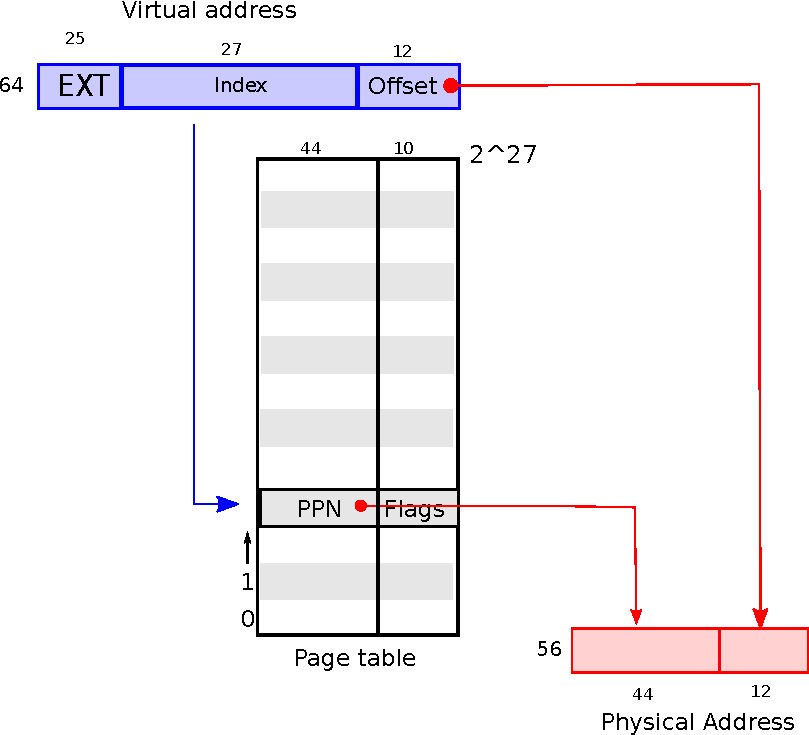
\includegraphics[scale=0.5]{fig/riscv_address.pdf}
\caption{RISC-V 虚拟和物理地址,具有简化的逻辑页表。  }
\label{fig:riscv_address}
\end{figure}     

xv6运行在Sv39 RISC-V上,这意味着只使用64位虚拟地址的底部39位;前 25 位未使用。在此 Sv39 配置中,RISC-V 页表逻辑上是    $2^{27}$    (134,217,728) 的数组
    \indextext{page table entries (PTEs)}    。每个 PTE 包含一个 44 位物理页号 (PPN) 和一些标志。分页硬件通过使用39位中的高27位索引到页表中找到PTE来翻译虚拟地址,并制作一个56位物理地址,其高44位来自PTE中的PPN,其低12位被复制来自原始虚拟地址。图~    \ref{fig:riscv_address}    通过将页表的逻辑视图显示为简单的 PTE 数组来显示此过程(有关更完整的情况,请参见图~    \ref{fig:riscv_pagetable}   )。页表使操作系统能够以 4096 (    $2^{12}$    ) 字节对齐块的粒度控制虚拟到物理地址转换。这样的块称为    \indextext{page}    。  

   \begin{figure}[t]
\center
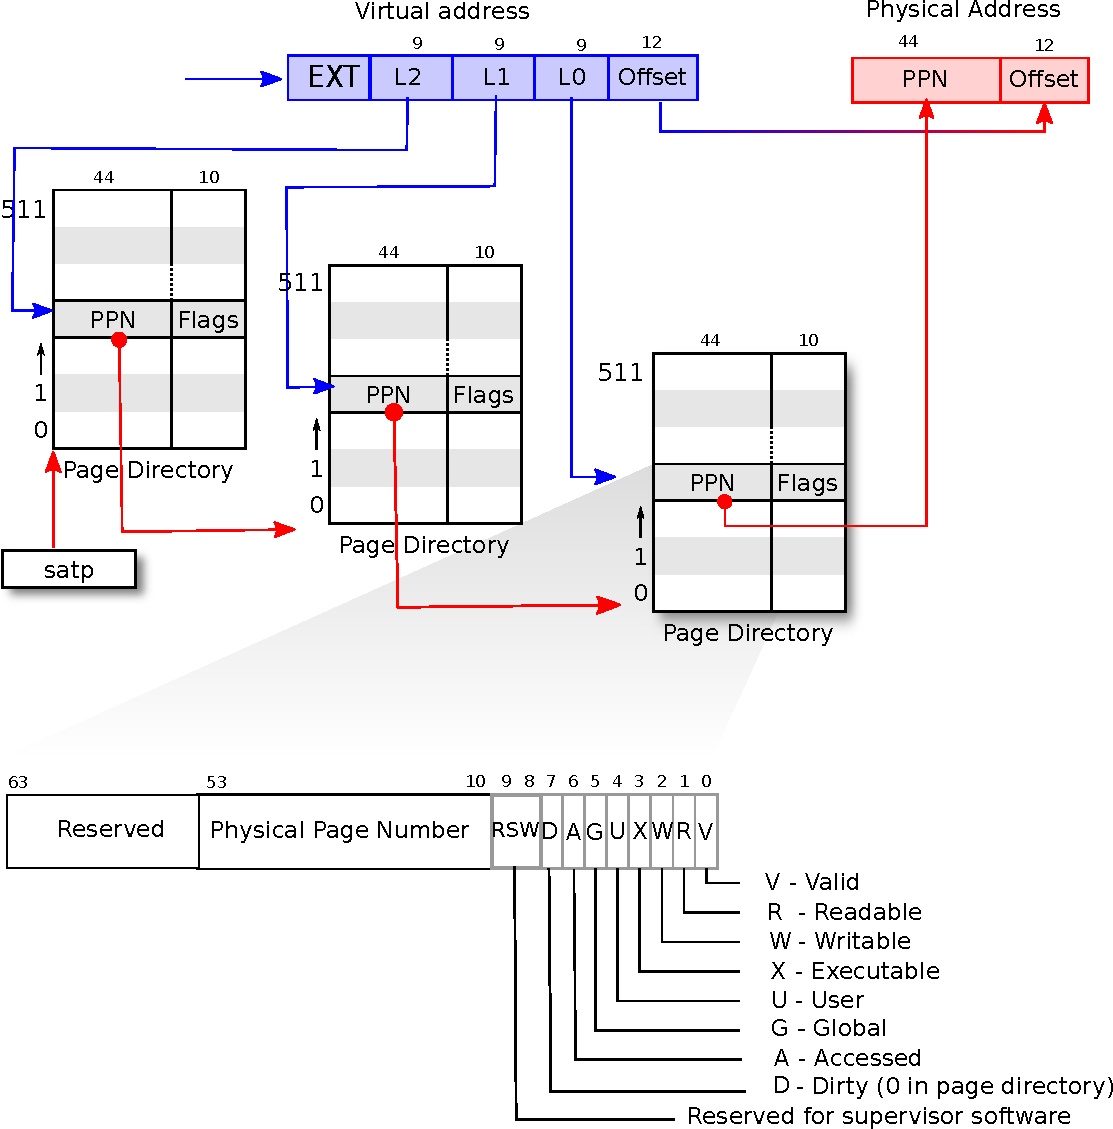
\includegraphics[scale=0.5]{fig/riscv_pagetable.pdf}
\caption{RISC-V 地址转换详细信息。  }
\label{fig:riscv_pagetable}
\end{figure}     

在 Sv39 RISC-V 中,虚拟地址的前 25 位不用于翻译。物理地址也有增长的空间:PTE 格式中有空间让物理页号再增长 10 位。 RISC-V 的设计者根据技术预测选择了这些数字。    $2^{39}$    字节为 512 GB,这对于在 RISC-V 计算机上运行的应用程序来说应该有足够的地址空间。    $2^{56}$    在不久的将来有足够的物理内存空间来容纳许多 I/O 设备和 DRAM 芯片。如果需要更多,RISC-V 设计人员已经定义了具有 48 位虚拟地址的 Sv48~    \cite{riscv:priv}    。  

如图~    \ref{fig:riscv_pagetable}    所示,RISC-V CPU 通过三个步骤将虚拟地址转换为物理地址。页表作为三层树存储在物理内存中。树的根是一个 4096 字节的页表页,包含 512 个 PTE,其中包含树的下一级页表页的物理地址。每个页面都包含树中最终级别的 512 个 PTE。分页硬件使用这 27 位中的前 9 位来选择根页表页中的 PTE,中间 9 位来选择树的下一级页表页中的 PTE,最后 9 位来选择期末PTE。 (在 Sv48 RISC-V 中,页表有四级,虚拟地址索引的位 39 到 47 位于顶层。)  

如果转换地址所需的三个 PTE 中的任何一个不存在,则分页硬件会引发    \indextext{page-fault exception}    ,将其留给内核来处理异常(请参阅第    \ref{CH:TRAP}    章)。  

与图~    \ref{fig:riscv_address}    的单层设计相比,图~    \ref{fig:riscv_pagetable}    的三层结构允许以内存高效的方式记录PTE。在大范围的虚拟地址没有映射的常见情况下,三级结构可以省略整个页目录。例如,如果应用程序仅使用从地址 0 开始的几个页,则顶级页目录的 1 到 511 项无效,并且内核不必为 511 中间页目录分配这些页。此外,内核也不必为那些 511 中间页目录的底层页目录分配页。因此,在本例中,三级设计为中间页目录保存了 511 个页面,
    $511\times512$    页面用于底层页面目录。  

尽管 CPU 在硬件中遍历三级结构作为执行加载或存储指令的一部分,但三级结构的潜在缺点是 CPU 必须从内存加载三个 PTE 来执行加载/存储指令中的虚拟地址到物理地址的转换。为了避免从物理内存加载 PTE 的成本,RISC-V CPU 将页表条目缓存在
    \indextext{Translation Look-aside Buffer (TLB)}    。  

每个 PTE 都包含标志位,这些标志位告诉分页硬件如何允许使用关联的虚拟地址。
    \indexcode{PTE_V}    指示 PTE 是否存在:如果未设置,则对该页面的引用会导致异常(即不允许)。
    \indexcode{PTE_R}    控制是否允许指令读取该页。
    \indexcode{PTE_W}    控制是否允许指令写入该页。
    \indexcode{PTE_X}    控制 CPU 是否可以将页面内容解释为指令并执行它们。
    \indexcode{PTE_U}    控制是否允许用户模式下的指令访问该页面;如果未设置    \indexcode{PTE_U}   ,则 PTE 只能在超级用户模式下使用。图~    \ref{fig:riscv_pagetable}    显示了它是如何工作的。标志和所有其他页面硬件相关的结构定义在
    \fileref{kernel/riscv.h}     

为了告诉CPU使用页表,内核必须将根页表页的物理地址写入
    \texttt{satp}       \index{satp@\lstinline{satp}}    寄存器。 CPU 将使用其自己的    \texttt{satp}    指向的页表来转换后续指令生成的所有地址。每个CPU都有自己的   \texttt{satp}   ,以便不同的CPU可以运行不同的进程,每个进程都有一个由自己的页表描述的私有地址空间。  

通常,内核将所有物理内存映射到其页表中,以便它可以使用加载/存储指令读取和写入物理内存中的任何位置。由于页目录位于物理内存中,因此内核可以通过使用标准存储指令写入 PTE 的虚拟地址来对页目录中的 PTE 内容进行编程。  

关于术语的一些注释。物理内存是指DRAM中的存储单元。物理内存的一个字节有一个地址,称为物理地址。指令仅使用虚拟地址,分页硬件将其转换为物理地址,然后发送到 DRAM 硬件以读取或写入存储。与物理内存和虚拟地址不同,虚拟内存不是物理对象,而是指内核提供的用于管理物理内存和虚拟地址的抽象和机制的集合。  

   \begin{figure}[h]
\centering
 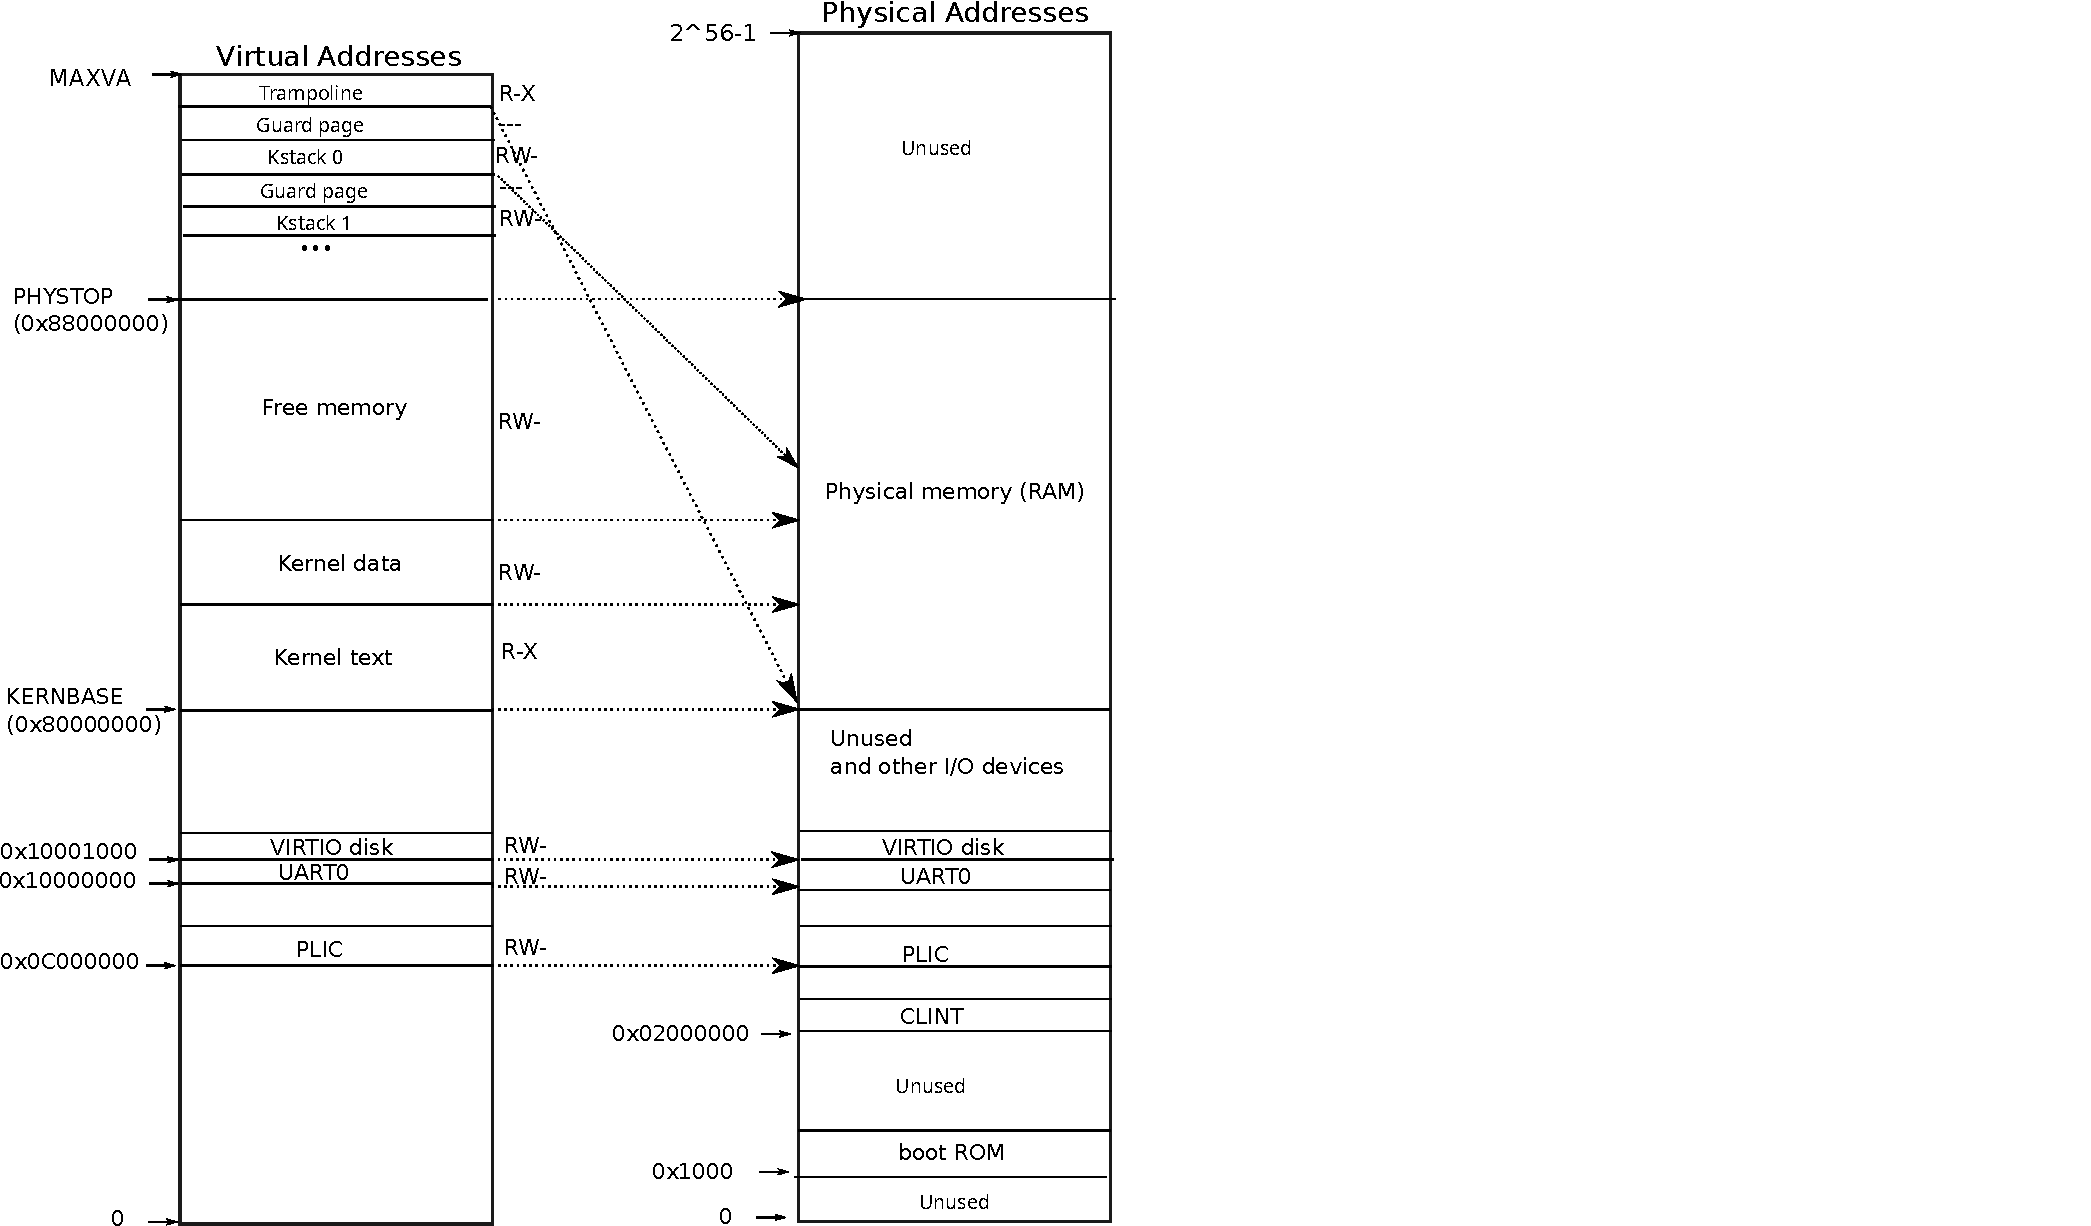
\includegraphics[scale=0.65]{fig/xv6_layout.pdf}
\caption{左边是 xv6 的内核地址空间。
  {    \sf       \small{RWX}      }  指 PTE 读、写和执行权限。右侧是 xv6 期望看到的 RISC-V 物理地址空间。  }
\label{fig:xv6_layout}
\end{figure}   
    \section{内核地址空间  }    Xv6 为每个进程维护一个页表,描述每个进程的用户地址空间,以及一个描述内核地址空间的页表。内核配置其地址空间的布局,以使其能够访问可预测虚拟地址的物理内存和各种硬件资源。图~    \ref{fig:xv6_layout}    显示了此布局如何将内核虚拟地址映射到物理地址。文件
    \fileref{kernel/memlayout.h}    声明 xv6 内核内存布局的常量。  

QEMU 模拟一台包含 RAM(物理内存)的计算机,该 RAM 从物理地址    \texttt{0x80000000}    开始,并至少持续到    \texttt{0x88000000}    ,xv6 称之为    \texttt{PHYSTOP}    。 QEMU 模拟还包括 I/O 设备,例如磁盘接口。 QEMU 将设备接口公开给软件:
    \indextext{memory-mapped}    控制寄存器位于下面
 物理地址空间中的    \texttt{0x80000000}   。内核可以通过读/写这些特殊的物理地址来与设备进行交互;此类读取和写入与设备硬件而不是 RAM 进行通信。 Chapter~    \ref{CH:TRAP}    解释展示 xv6 与设备的交互。  

内核使用“直接映射”获取 RAM 和内存映射设备寄存器;即将资源映射到等于物理地址的虚拟地址。例如,内核本身在虚拟地址空间和物理内存中都位于    \lstinline{KERNBASE=0x80000000}   。直接映射简化了读取或写入物理内存的内核代码。例如,当   \lstinline{fork}   为子进程分配用户内存时,分配器返回该内存的物理地址;
    \lstinline{fork}    在将父进程的用户内存复制到子进程时直接使用该地址作为虚拟地址。  

有几个未直接映射的内核虚拟地址:  

   \begin{itemize}

 
   \item   trampoline 页。它映射在虚拟地址空间的顶部;用户页表具有相同的映射。 Chapter~    \ref{CH:TRAP}    讨论了 trampoline 页的作用,但我们在这里看到了页表的一个有趣的用例;物理页(保存 trampoline 代码)在内核的虚拟地址空间中映射两次:一次在虚拟地址空间的顶部,一次是直接映射。   \item   内核堆栈页。每个进程都有自己的内核堆栈,该堆栈被映射到高位,以便在其下方 xv6 可以留下未映射的    \indextext{guard
    page}    。保护页面的 PTE 无效(即
    \lstinline{PTE_V}    未设置),因此如果内核溢出内核堆栈,很可能会导致异常并且内核会出现Panic。如果没有保护页,溢出的堆栈将覆盖其他内核内存,从而导致不正确的操作。Panic崩溃是更好的选择。  \end{itemize}     

虽然内核通过高内存映射使用其堆栈,但内核也可以通过直接映射地址访问它们。另一种设计可能只有直接映射,并在直接映射地址处使用堆栈。然而,在这种安排中,提供保护页将涉及取消虚拟地址的映射,否则这些虚拟地址将引用物理内存,从而难以使用。  

内核使用权限映射 trampoline 页面和内核文本
    \lstinline{PTE_R}    和
    \lstinline{PTE_X}    。内核从这些页面读取并执行指令。内核将其他页面映射到权限
    \lstinline{PTE_R}    和
    \lstinline{PTE_W}    ,以便它可以读写这些页面中的内存。保护页的映射无效。
    \section{代码:创建地址空间  }     

大多数用于操作地址空间和页表的 xv6 代码都驻留在  {    \tt    vm.c   }  中
    \lineref{kernel/vm.c:1}    。中心数据结构是  {    \tt    pagetable\_t   }  ,它实际上是指向 RISC-V 根页表页的指针; {    \tt    pagetable\_t   }  可以是内核页表,也可以是每进程页表之一。核心功能是  {    \tt    walk   }  ,它查找虚拟地址的 PTE ,以及  {    \tt    mappages   }  ,它为新映射安装 PTE 。以  {    \tt    kvm   }  开头的函数操作内核页表;以  {    \tt    uvm   }  开头的函数操作用户页表;两者都使用其他功能。
  {    \tt    copyout   }  和  {    \tt    copyin   }  将数据复制到作为系统调用参数提供的用户虚拟地址;它们位于  {    \tt    vm.c   }  中,因为它们需要显式转换这些地址才能找到相应的物理内存。  

在启动顺序的早期,
    \indexcode{main}    次调用
    \indexcode{kvminit}   
    \lineref{kernel/vm.c:/^kvminit/}    使用以下命令创建内核的页表
    \indexcode{kvmmake}   
    \lineref{kernel/vm.c:/^kvmmake/}    。此调用发生在 xv6 在 RISC-V 上启用分页之前,因此地址直接引用物理内存。
    \lstinline{kvmmake}    首先分配物理内存页来保存根页表页。然后它调用
    \indexcode{kvmmap}    安装内核所需的翻译。翻译包括内核的指令和数据、物理内存高达
    \indexcode{PHYSTOP}    和实际上是设备的内存范围。
    \indexcode{proc_mapstacks}   
    \lineref{kernel/proc.c:/^proc_mapstacks/}    为每个进程分配一个内核堆栈。它调用    \lstinline{kvmmap}    将每个堆栈映射到由
    \lstinline{KSTACK}    ,为无效的堆栈保护页留出空间。  

   \indexcode{kvmmap}   
    \lineref{kernel/vm.c:/^kvmmap/}    调用
    \indexcode{mappages}   
    \lineref{kernel/vm.c:/^mappages/}    ,它将一系列虚拟地址到相应物理地址范围的映射安装到页表中。它以页面间隔为范围内的每个虚拟地址单独执行此操作。对于每个要映射的虚拟地址,
    \lstinline{mappages}    调用
    \indexcode{walk}    查找该地址的 PTE 地址。然后它初始化 PTE 以保存相关的物理页码、所需的权限(    \lstinline{PTE_W}    、
    \lstinline{PTE_X}    和/或
    \lstinline{PTE_R}    ),以及
    \lstinline{PTE_V}    将 PTE 标记为有效
    \lineref{kernel/vm.c:/perm...PTE_V/}    。  

   \indexcode{walk}   
    \lineref{kernel/vm.c:/^walk/}    模仿 RISC-V 分页硬件,因为它在 PTE 中查找虚拟地址(见图    \ref{fig:riscv_pagetable}   )。
    \lstinline{walk}    此时将 3 级页表下降 9 位。它使用每级的 9 位虚拟地址来查找下一级页表或最终页的 PTE
    \lineref{kernel/vm.c:/pte.=..pagetable/}    。如果 PTE 无效,则所需的页面尚未分配;如果
    \lstinline{alloc}    参数已设置,
    \lstinline{walk}    分配一个新的页表页并将其物理地址放入 PTE 中。它返回树中最底层的PTE的地址
    \lineref{kernel/vm.c:/return..pagetable/}   。  

上面的代码依赖于直接映射到内核虚拟地址空间的物理内存。例如,当    \lstinline{walk}    降低页表的级别时,它会从 PTE    \lineref{kernel/vm.c:/pagetable.=..pa.*E2P/}    中提取下一级页表的(物理)地址,然后使用该地址作为虚拟地址来获取下一级的 PTE
    \lineref{kernel/vm.c:/t..pte.=..paget/}    。  

   \indexcode{main}    次调用
    \indexcode{kvminithart}   
    \lineref{kernel/vm.c:/^kvminithart/}    安装内核页表。它将根页表页的物理地址写入寄存器
    \texttt{satp}    。此后,CPU 将使用内核页表转换地址。由于内核使用恒等映射,因此下一条指令的现在虚拟地址将映射到正确的物理内存地址。  

每个 RISC-V CPU 将页表条目缓存在一个
    \indextext{Translation Look-aside Buffer (TLB)}    ,当 xv6 更改页表时,它必须告诉 CPU 使相应的缓存 TLB 条目无效。如果没有,那么在稍后的某个时刻,TLB 可能会使用旧的缓存映射,指向同时已分配给另一个进程的物理页,因此,进程可能能够在其他进程的内存上乱写乱画。 RISC-V 有一条指令    \indexcode{sfence.vma}   ,用于刷新当前 CPU 的 TLB。 Xv6重新加载后在 {    \tt    kvminithart   } 中执行 {    \tt    sfence.vma   } 
    \texttt{satp}   寄存器,以及在返回用户空间之前切换到用户页表的trampoline代码中
    \lineref{kernel/trampoline.S:/sfence.vma/}    。  

更改前还需要发出    \texttt{sfence.vma}   
    \texttt{satp}    ,以便等待所有未完成的加载和存储完成。这一等待可确保先前对页表的更新已完成,并确保先前的加载和存储使用旧页表,而不是新页表。  

为了避免刷新整个 TLB,RISC-V CPU 可能支持地址空间标识符 (ASID)~    \cite{riscv:priv}    。然后内核可以仅刷新特定地址空间的 TLB 条目。 Xv6没有使用这个功能。  

   \section{物理内存分配  }     

内核必须在运行时为页表、用户内存、内核堆栈和管道缓冲区分配和释放物理内存。  

xv6 使用内核末尾和
    \indexcode{PHYSTOP}    用于运行时分配。它一次分配和释放整个 4096 字节页面。它通过将链接列表穿过页面本身来跟踪哪些页面是空闲的。分配包括从链表中删除页面;释放包括将释放的页面添加到列表中。
    \section{代码:物理内存分配器  }     

分配器驻留在  {    \tt    kalloc.c   }     \lineref{kernel/kalloc.c:1}    中。分配器的数据结构是可用于分配的物理内存页的空闲列表。每个空闲页面的列表元素是
    \indexcode{struct run}   
    \lineref{kernel/kalloc.c:/^struct.run/}    。分配器从哪里获取内存来保存该数据结构?它存储每个免费页面的
 空闲页面本身中的    \lstinline{run}    结构,因为那里没有存储任何其他内容。空闲列表受自旋锁保护
    \linerefs{kernel/kalloc.c:/^struct.{/,/}/}    。列表和锁包装在一个结构中,以明确锁保护结构中的字段。现在,忽略锁和调用
    \lstinline{acquire}    和
    \lstinline{release}   ;第~    \ref{CH:LOCK}    章将详细研究锁定。  

功能
    \indexcode{main}    次调用
    \indexcode{kinit}    初始化分配器
    \lineref{kernel/kalloc.c:/^kinit/}    。
    \lstinline{kinit}    初始化空闲列表以保存内核末尾和  {    \tt    PHYSTOP   }  之间的每个页面。 Xv6 应该通过解析硬件提供的配置信息来确定有多少物理内存可用。相反,xv6 假设机器有 128 MB RAM。
    \lstinline{kinit}    调用
    \indexcode{freerange}    通过每页调用将内存添加到空闲列表
    \indexcode{kfree}    。 PTE 只能引用在 4096 字节边界(是 4096 的倍数)上对齐的物理地址,因此
    \lstinline{freerange}    使用
    \indexcode{PGROUNDUP}    以确保它仅释放对齐的物理地址。分配器在没有内存的情况下启动;这些调用
    \lstinline{kfree}    给它一些管理。  

分配器有时将地址视为整数,以便对它们执行算术(例如,遍历
    \lstinline{freerange}    ),有时使用地址作为读写内存的指针(例如,操纵
    \lstinline{run}    结构存储在每个页中);这种地址的双重使用是分配器代码充满 C 类型转换的主要原因。
    \index{type cast}    另一个原因是释放和分配本质上改变了内存的类型。  

功能
    \lstinline{kfree}   
    \lineref{kernel/kalloc.c:/^kfree/}    首先将要释放的内存中的每个字节设置为值 1。这将导致在释放内存后使用内存的代码(使用“悬空引用”)读取垃圾而不是旧的有效内容;希望这会导致这样的代码打破得更快。然后
    \lstinline{kfree}    将页面添加到空闲列表之前:它进行强制转换
    \lstinline{pa}    指向的指针
    \lstinline{struct}   
    \lstinline{run}    ,记录空闲列表的旧开始
    \lstinline{r->next}    ,并将空闲列表设置为
    \lstinline{r}   。
    \indexcode{kalloc}    删除并返回空闲列表中的第一个元素。  

   \section{进程地址空间  }     

每个进程都有一个单独的页表,当xv6在进程之间切换时,它也会更改页表。图~    \ref{fig:processlayout}    比图~    \ref{fig:as}    更详细地显示了进程的地址空间。进程的用户内存从虚拟地址 0 开始,可以增长到    \texttt{MAXVA}   
    \lineref{kernel/riscv.h:/MAXVA/}    ,原则上允许进程寻址 256 GB 内存。  

进程的地址空间由包含程序文本的页面组成(xv6 使用权限    \lstinline{PTE_R}    进行映射,
    \lstinline{PTE_X}    和    \lstinline{PTE_U}    ),包含程序预初始化数据的页面、堆栈页面和堆页面。 Xv6将数据、栈、堆与权限进行映射
    \lstinline{PTE_R}    、    \lstinline{PTE_W}    和    \lstinline{PTE_U}    。  

在用户地址空间内使用权限是强化用户进程的常用技术。如果文本被映射为
    \lstinline{PTE_W}    ,那么进程可能会意外修改自己的程序;例如,编程错误可能会导致程序写入空指针,修改地址 0 处的指令,然后继续运行,这可能会造成更多破坏。为了立即检测此类错误,xv6 映射不带    \lstinline{PTE_W}    的文本;如果程序意外地尝试存储到地址 0,硬件将拒绝执行存储并引发页错误(请参阅第    \ref{sec:pagefaults}    节)。然后内核终止该进程并打印出一条信息性消息,以便开发人员可以追踪问题。  

类似地,通过在没有    \lstinline{PTE_X}    的情况下映射数据,用户程序不会意外跳转到程序数据中的某个地址并在该地址开始执行。  

在现实世界中,通过仔细设置权限来强化流程也有助于防御安全攻击。对手可能会向程序(例如 Web 服务器)提供精心构造的输入,从而触发程序中的错误,希望将该错误转化为漏洞利用~    \cite{aleph:smashing}    。仔细设置权限和其他技术(例如随机化用户地址空间的布局)会使此类攻击更加困难。  

堆栈是一个单页,并显示由 exec 创建的初始内容。包含命令行参数的字符串以及指向它们的指针数组位于堆栈的最顶部。就在其下方是允许程序启动的值
    \lstinline{main}    就像函数    \lstinline{main(argc}    一样,
    \lstinline{argv)}    刚刚被调用。  

为了检测用户堆栈溢出分配的堆栈内存,xv6 通过清除    \lstinline{PTE_U}    标志在堆栈正下方放置一个不可访问的保护页。如果用户堆栈溢出并且进程尝试使用堆栈下方的地址,则硬件将生成页面错误异常,因为在用户模式下运行的程序无法访问保护页。现实世界的操作系统可能会在用户堆栈溢出时自动为其分配更多内存。  

当进程向 xv6 请求更多用户内存时,xv6 会增加进程的堆。 Xv6首先使用 {    \tt    kalloc   } 来分配物理页。然后它将 PTE 添加到指向新物理页的进程页表中。 Xv6 设置
    \lstinline{PTE_W}    ,
    \lstinline{PTE_R}    ,
    \lstinline{PTE_U}    和
 这些 PTE 中的    \lstinline{PTE_V}    标志。大多数进程不使用整个用户地址空间;xv6 离开
    \lstinline{PTE_V}    在未使用的 PTE 中清除。  

我们在这里看到一些使用页表的很好的例子。首先,不同进程的页表将用户地址转换为不同的物理内存页,从而每个进程都拥有私有的用户内存。其次,每个进程将其内存视为具有从零开始的连续虚拟地址,而进程的物理内存可以是不连续的。第三,内核用trampoline代码映射一个页面到用户地址空间的顶部(没有
    \lstinline{PTE_U}    ),因此单页物理内存显示在所有地址空间中,但只能由内核使用。  

   \begin{figure}[t]
\center
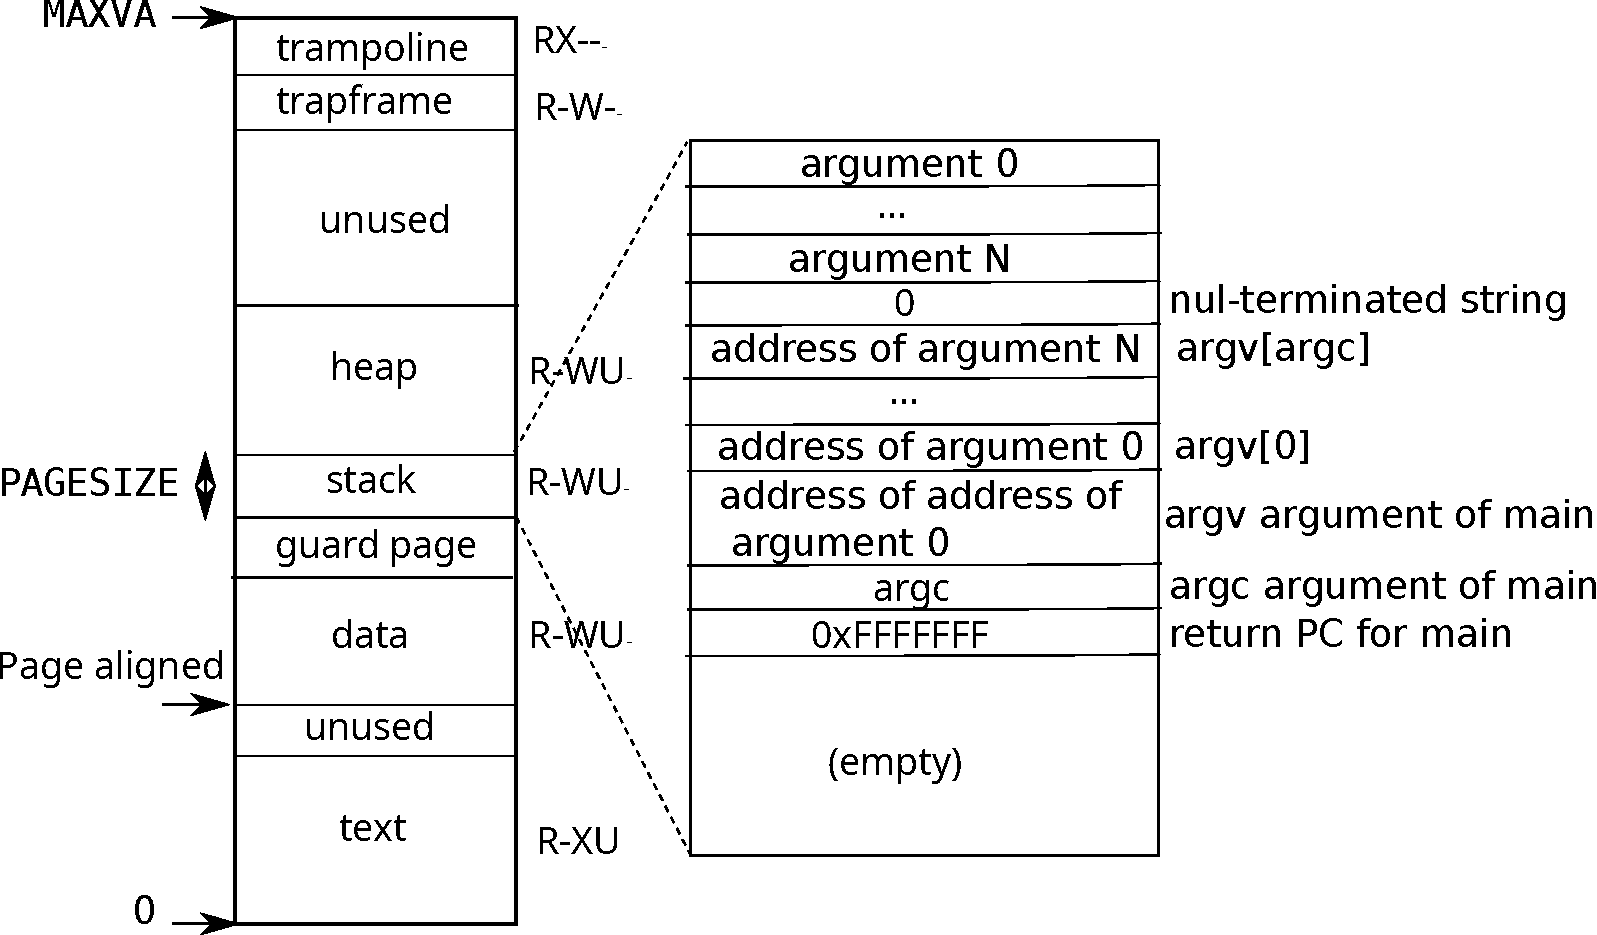
\includegraphics[scale=0.5]{fig/processlayout.pdf}
\caption{进程的用户地址空间及其初始堆栈。  }
\label{fig:processlayout}
\end{figure}     

   \section{代码:sbrk  }     

   \lstinline{sbrk}    是进程收缩或增加其内存的系统调用。系统调用是通过函数实现的
    \lstinline{growproc}   
    \lineref{kernel/proc.c:/^growproc/}    。
    \lstinline{growproc}    调用    \lstinline{uvmalloc}    或
    \lstinline{uvmdealloc}    ,取决于    \lstinline{n}    是正数还是负数。
    \lstinline{uvmalloc}   
    \lineref{kernel/vm.c:/^uvmalloc/}    使用  {    \tt    kalloc   }  分配物理内存,并使用  {    \tt    mappages   }  将 PTE 添加到用户页表中。
    \lstinline{uvmdealloc}    调用
  {    \tt    uvmunmap   } 
  \lineref{kernel/vm.c:/^uvmunmap/}   ,它使用  {    \tt    work   }  查找 PTE 和
  {    \tt    kfree   }  释放它们引用的物理内存。  

Xv6 使用进程的页表不仅告诉硬件如何映射用户虚拟地址,而且还作为将哪些物理内存页分配给该进程的唯一记录。这就是释放用户内存(在  {    \tt    uvmunmap   }  中)需要检查用户页表的原因。
    \section{代码:执行  }   
    \lstinline{exec}    是一个系统调用,它用从文件(称为二进制文件或可执行文件)读取的数据替换进程的用户地址空间。二进制文件通常是编译器和链接器的输出,并保存机器指令和程序数据。
    \lstinline{exec}       \lineref{kernel/exec.c:/^exec/}     使用    \indexcode{namei}    打开命名的二进制文件    \lstinline{path}   
    \lineref{kernel/exec.c:/namei/}   ,在 Chapter~    \ref{CH:FS}    中进行了解释。然后,它读取 ELF 标头。 Xv6 二进制文件采用广泛使用的    \indextext{ELF format}    格式,定义于
    \fileref{kernel/elf.h}    。 ELF 二进制文件由 ELF 标头组成,
    \indexcode{struct elfhdr}       \lineref{kernel/elf.h:/^struct.elfhdr/}    ,后跟一系列程序段标头,
    \lstinline{struct proghdr}       \lineref{kernel/elf.h:/^struct.proghdr/}   。每个
    \lstinline{progvhdr}    描述了必须加载到内存中的应用程序部分; xv6 程序有两个程序节头:一个用于指令,一个用于数据。  

第一步是快速检查该文件是否可能包含 ELF 二进制文件。 ELF 二进制文件以四字节“幻数”开头
    \lstinline{0x7F}    ,
    \lstinline{`E'}    ,
    \lstinline{`L'}    ,
    \lstinline{`F'}   ,或
    \indexcode{ELF_MAGIC}   
    \lineref{kernel/elf.h}{3}    。如果 ELF header 有正确的幻数,
    \lstinline{exec}    假定二进制文件格式良好。  

   \lstinline{exec}    分配一个没有用户映射的新页表
    \indexcode{proc_pagetable}   
    \lineref{kernel/exec.c:/proc_pagetable/}    ,为每个 ELF 段分配内存
    \indexcode{uvmalloc}   
    \lineref{kernel/exec.c:/uvmalloc/}    ,并将每个段加载到内存中
    \indexcode{loadseg}   
    \lineref{kernel/exec.c:/loadseg/}    。
    \lstinline{loadseg}    使用
    \indexcode{walkaddr}    查找要写入 ELF 段的每个页面的已分配内存的物理地址,以及
    \indexcode{readi}    从文件中读取。  

程序节标题为
    \indexcode{/init}   ,第一个用户程序创建
    \lstinline{exec}    ,看起来像这样:
    \begin{footnotesize}
\begin{verbatim}
# objdump -p user/_init

user/_init:     file format elf64-little

Program Header:
0x70000003 off    0x0000000000006bb0 vaddr 0x0000000000000000
                                       paddr 0x0000000000000000 align 2**0
         filesz 0x000000000000004a memsz 0x0000000000000000 flags r--
    LOAD off    0x0000000000001000 vaddr 0x0000000000000000
                                       paddr 0x0000000000000000 align 2**12
         filesz 0x0000000000001000 memsz 0x0000000000001000 flags r-x
    LOAD off    0x0000000000002000 vaddr 0x0000000000001000
                                       paddr 0x0000000000001000 align 2**12
         filesz 0x0000000000000010 memsz 0x0000000000000030 flags rw-
   STACK off    0x0000000000000000 vaddr 0x0000000000000000
                                       paddr 0x0000000000000000 align 2**4
         filesz 0x0000000000000000 memsz 0x0000000000000000 flags rw-
\end{verbatim}
\end{footnotesize}     

我们看到文本段应该从文件中偏移量 0x1000 处的内容加载到内存中的虚拟地址 0x0(没有写权限)。我们还看到数据应该加载到地址 0x1000,该地址位于页边界,并且没有可执行权限。  

程序节标题
    \lstinline{filesz}    可能小于
    \lstinline{memsz}    ,表示它们之间的间隙应该用零填充(对于 C 全局变量)而不是从文件中读取。为了
    \lstinline{/init}    ,数据
    \lstinline{filesz}    是 0x10 字节并且
    \lstinline{memsz}    是 0x30 字节,因此
    \indexcode{uvmalloc}    分配足够的物理内存来容纳 0x30 字节,但仅从文件中读取 0x10 字节
    \lstinline{/init}    。  

现在
    \indexcode{exec}    分配并初始化用户堆栈。它只分配一个堆栈页。
    \lstinline{exec}    将参数字符串一次复制到堆栈顶部,并将指向它们的指针记录在
    \indexcode{ustack}    。它将一个空指针放置在将要执行的内容的末尾
    \indexcode{argv}    列表传递到
    \lstinline{main}    。中的前三个条目
    \lstinline{ustack}    是假返回程序计数器,
    \indexcode{argc}    和
    \lstinline{argv}    指针。  

   \lstinline{exec}    在堆栈页正下方放置了一个不可访问的页,因此尝试使用多个页的程序将会出错。这个无法访问的页面还允许
    \lstinline{exec}    处理太大的参数;在这种情况下,
    \indexcode{copyout}   
    \lineref{kernel/vm.c:/^copyout/}    函数
    \lstinline{exec}    用于将参数复制到堆栈时会注意到目标页面不可访问,并将返回 -1。  

在准备新的内存映像期间,如果
    \lstinline{exec}    检测到错误,例如无效的程序段,它跳转到标签
    \lstinline{bad}    ,释放新图像,并返回-1。
    \lstinline{exec}    必须等待释放旧映像,直到确定系统调用将成功:如果旧映像消失,系统调用无法向其返回 -1。唯一的错误情况是
    \lstinline{exec}    在图像创建期间发生。图像完成后,
    \lstinline{exec}   可以提交到新页表
    \lineref{kernel/exec.c:/pagetable.=.pagetable/}    并释放旧的
    \lineref{kernel/exec.c:/proc_freepagetable/}    。  

   \lstinline{exec}    将 ELF 文件中的字节加载到内存中 ELF 文件指定的地址处。用户或进程可以将他们想要的任何地址放入 ELF 文件中。因此
    \lstinline{exec}    是有风险的,因为 ELF 文件中的地址可能无意或有意地引用内核。粗心的内核所造成的后果可能包括从崩溃到恶意破坏内核隔离机制(即安全漏洞)。 Xv6 执行许多检查来避免这些风险。例如
    \lstinline{if(ph.vaddr + ph.memsz < ph.vaddr)}    检查总和是否溢出 64 位整数。危险在于用户可以使用以下命令构建 ELF 二进制文件:
    \lstinline{ph.vaddr}    指向用户选择的地址,并且
    \lstinline{ph.memsz}    足够大,总和会溢出到 0x1000,这看起来像是有效值。在旧版本的 xv6 中,用户地址空间也包含内核(但在用户模式下不可读写),用户可以选择与内核内存相对应的地址,从而将数据从 ELF 二进制文件复制到内核中。在 xv6 的 RISC-V 版本中,这种情况不会发生,因为内核有自己独立的页表;
    \lstinline{loadseg}    加载到进程的页表中,而不是加载到内核的页表中。  

内核开发人员很容易忽略关键的检查,并且现实世界的内核长期以来一直缺少检查,用户程序可以利用这些检查的缺失来获取内核权限。 xv6 很可能没有完成验证提供给内核的用户级数据的完整工作,恶意用户程序可能能够利用这些数据来规避 xv6 的隔离。
    \section{真实世界  }     

与大多数操作系统一样,xv6 使用分页硬件进行内存保护和映射。大多数操作系统通过结合分页和页错误异常来比 xv6 更复杂地使用分页,我们将在第    \ref{CH:TRAP}    章中讨论这一点。  

Xv6 的简化是通过内核使用虚拟地址和物理地址之间的直接映射,并假设在地址 0x8000000 处存在物理 RAM,这是内核期望加载的位置。这适用于 QEMU,但在真实硬件上,事实证明这是一个坏主意;真实硬件将 RAM 和设备放置在不可预测的物理地址处,因此(例如)0x8000000 处可能没有 RAM,xv6 期望能够在此处存储核心。更严格的内核设计利用页表将任意硬件物理内存布局转换为可预测的内核虚拟地址布局。  

RISC-V支持物理地址级别的保护,但xv6没有使用该功能。  

在具有大量内存的计算机上,使用 RISC-V 对“超级页面”的支持可能很有意义。当物理内存较小时,小页面很有意义,以允许以细粒度分配和页出到磁盘。例如,如果一个程序仅使用 8 KB 内存,则为其提供整个 4 MB 物理内存超级页面是一种浪费。较大的页面对于具有大量 RAM 的机器来说是有意义的,并且可以减少页表操作的开销。  

xv6 内核缺少可以为小对象提供内存的类似  {    \tt    malloc   }  的分配器,从而阻止内核使用需要动态分配的复杂数据结构。更复杂的内核可能会分配许多不同大小的小块,而不是(如在 xv6 中)仅 4096 字节块;真正的内核分配器需要处理小分配和大分配。  

内存分配是一个长期的热门话题,基本问题是有效利用有限的内存并为未知的未来请求做好准备~    \cite{knuth}    。如今,人们更关心速度而不是空间效率。
    \section{练习  }     

   \begin{enumerate}

 
   \item   解析 RISC-V 的设备树以查找计算机拥有的物理内存量。   \item   编写一个用户程序,通过调用将其地址空间增加一个字节
    \lstinline{sbrk(1)}    。运行程序并在调用之前调查程序的页表
    \lstinline{sbrk}    和调用之后
    \lstinline{sbrk}    。内核分配了多少空间?新内存的 PTE 包含什么?   \item   修改 xv6 以对内核使用超级页面。   \item   Unix 实现
    \lstinline{exec}    传统上包括对 shell 脚本的特殊处理。如果要执行的文件以文本开头
    \lstinline{#!}    ,则第一行被视为要运行以解释文件的程序。例如,如果
 调用   \lstinline{exec}   运行
    \lstinline{myprog}   
    \lstinline{arg1}    和
    \lstinline{myprog}    的第一行是
    \lstinline{#!/interp}   ,那么
    \lstinline{exec}    运行
 带命令行的    \lstinline{/interp}   
    \lstinline{/interp}   
    \lstinline{myprog}   
    \lstinline{arg1}    。在 xv6 中实现对此约定的支持。   \item   为内核实现地址空间布局随机化。  \end{enumerate}     


   
    
\documentclass[UTF8]{article}
\usepackage{xeCJK}
\usepackage{amsmath,amssymb}
\begin{document}

   \chapter{Traps and system calls}   
    \label{CH:TRAP}     

共有三种事件导致 CPU 搁置普通指令执行并强制将控制权转移到处理该事件的特殊代码。一种情况是系统调用,当用户程序执行  {    \tt    紧急呼叫   }  指令以要求内核为其执行某些操作时。另一种情况是    \indextext{exception}    :指令(用户或内核)执行非法操作,例如除以零或使用无效的虚拟地址。第三种情况是设备    \indextext{interrupt}    ,当设备发出需要注意的信号时,例如当磁盘硬件完成读取或写入请求时。  

本书使用    \indextext{trap}    作为这些情况的通用术语。通常,陷阱发生时正在执行的任何代码稍后都需要恢复,并且不需要知道发生了任何特殊情况。也就是说,我们经常希望陷阱是透明的;这对于设备中断尤其重要,而被中断的代码通常不会预料到这种情况。通常的顺序是陷阱强制将控制权转移到内核中;内核保存寄存器和其他状态,以便可以恢复执行;内核执行适当的处理程序代码(例如,系统调用实现或设备驱动程序);内核恢复保存的状态并从陷阱中返回;原始代码从中断处继续。  

xv6 处理内核中的所有陷阱;陷阱不会传递给用户代码。对于系统调用来说,处理内核中的陷阱是很自然的。这对于中断来说是有意义的,因为隔离要求仅允许内核使用设备,并且因为内核是在多个进程之间共享设备的便捷机制。它对于异常也有意义,因为 xv6 通过杀死有问题的程序来响应用户空间的所有异常。  

Xv6 陷阱处理分四个阶段进行:RISC-V CPU 采取的硬件操作、为内核 C 代码做好准备的一些汇编指令、决定如何处理陷阱的 C 函数以及系统调用或设备驱动程序服务例程。虽然三种陷阱类型之间的共性表明内核可以使用单个代码路径处理所有陷阱,但事实证明,对于三种不同的情况使用单独的代码会很方便:来自用户空间的陷阱、来自内核空间的陷阱和计时器中断。处理陷阱的内核代码(汇编程序或 C)通常称为    \indextext{handler}    ;第一个处理程序指令通常用汇编程序(而不是 C)编写,有时称为    \indextext{vector}    。  

   \section{RISC-V陷阱机械  }     

每个 RISC-V CPU 都有一组控制寄存器,内核写入这些控制寄存器来告诉 CPU 如何处理陷阱,并且内核可以读取这些寄存器来找出已发生的陷阱。 RISC-V 文档包含完整的故事~    \cite{riscv:priv}    。  {    \tt    riscv.h   } 
    \lineref{kernel/riscv.h:1}    包含 xv6 使用的定义。以下是最重要寄存器的概述:  

   \begin{itemize}


   \item      \indexcode{stvec}    :内核将其陷阱处理程序的地址写入此处; RISC-V 跳转到  {    \tt    stvec   }  中的地址来处理陷阱。   \item      \indexcode{sepc}    :当陷阱发生时,RISC-V 将程序计数器保存在这里(因为  {    \tt    件   }  随后会被  {    \tt    stvec   }  中的值覆盖)。这
  {    \tt    sret   } (从陷阱返回)指令将  {    \tt    单独   }  复制到
  {    \tt    件   }  。内核可以编写  {    \tt    单独   }  来控制  {    \tt    sret   }  的去向。   \item      \indexcode{scause}   :RISC-V 在此处放置一个数字来描述陷阱的原因。   \item      \indexcode{sscratch}    :陷阱处理程序代码使用  {    \tt    scratch   }  来帮助避免在保存用户寄存器之前覆盖它们。   \item      \indexcode{sstatus}   : {    \tt    状态   }  中的 SIE 位控制是否启用设备中断。如果内核清除 SIE,RISC-V 将推迟设备中断,直到内核设置 SIE。 SPP 位指示陷阱是来自用户模式还是管理模式,并控制  {    \tt    sret   }  返回的模式。  \end{itemize}     

上述寄存器与管理模式下处理的陷阱相关,并且不能在用户模式下读取或写入。对于机器模式下处理的陷阱,有一组类似的控制寄存器; xv6 仅将它们用于定时器中断的特殊情况。  

多核芯片上的每个 CPU 都有自己的一组寄存器,并且在任何给定时间都可能有多个 CPU 正在处理陷阱。  

当需要强制陷阱时,RISC-V 硬件会对所有陷阱类型(定时器中断除外)执行以下操作:  

   \begin{enumerate}


   \item   如果陷阱是设备中断,并且  {    \tt    状态   }  SIE 位清零,则不要执行以下任何操作。   \item   通过清除  {    \tt    状态   }  中的 SIE 位来禁用中断。   \item   将  {    \tt    件   }  复制到  {    \tt    单独   }  。   \item   将当前模式(用户或管理员)保存在  {    \tt    状态   }  的 SPP 位中。   \item   设置  {    \tt   原因   }  以反映陷阱的原因。   \item   将模式设置为主管。   \item   将  {    \tt    stvec   }  复制到  {    \tt    件   }  。   \item   在新的  {    \tt    件   }  处开始执行。  \end{enumerate}     

请注意,CPU 不会切换到内核页表,不会切换到内核中的堆栈,并且不会保存除  {    \tt    件   }  之外的任何寄存器。内核软件必须执行这些任务。 CPU 在陷阱期间执行最少工作的原因之一是为软件提供灵活性。例如,某些操作系统在某些情况下省略页表切换以提高陷阱性能。  

值得思考是否可以省略上面列出的任何步骤,也许是为了寻找更快的陷阱。尽管在某些情况下可以使用更简单的顺序,但一般来说,省略许多步骤是危险的。例如,假设 CPU 没有切换程序计数器。然后,来自用户空间的陷阱可以切换到管理员模式,同时仍然运行用户指令。这些用户指令可能会破坏用户/内核隔离,例如通过修改  {    \tt    卫星   }  寄存器以指向允许访问所有物理内存的页表。因此,CPU 切换到内核指定的指令地址(即  {    \tt    stvec   }  )非常重要。  

   \section{来自用户空间的陷阱  }     

Xv6 对陷阱的处理方式有所不同,具体取决于陷阱是在内核中执行还是在用户代码中执行时发生。这是来自用户代码的陷阱的故事;部分~    \ref{s:ktraps}    描述了内核代码中的陷阱。  

如果用户程序进行系统调用( {    \tt    紧急呼叫   }  指令)、执行非法操作或者设备中断,则在用户空间执行时可能会发生陷阱。来自用户空间的陷阱的高级路径是
  {    \tt    用户向量   } 
    \lineref{kernel/trampoline.S:/^uservec/}   ,然后  {    \tt    用户陷阱   } 
    \lineref{kernel/trap.c:/^usertrap/}    ;返回时,
  {    \tt    用户陷阱   } 
    \lineref{kernel/trap.c:/^usertrapret/}    然后
  {    \tt    用户名   } 
    \lineref{kernel/trampoline.S:/^userret/}    。  

xv6 陷阱处理设计的一个主要限制是 RISC-V 硬件在强制陷阱时不会切换页表。这意味着  {    \tt    stvec   }  中的陷阱处理程序地址必须在用户页表中具有有效的映射,因为这是陷阱处理代码开始执行时有效的页表。此外,xv6的陷阱处理代码需要切换到内核页表;为了能够在该切换后继续执行,内核页表还必须具有  {    \tt    stvec   }  指向的处理程序的映射。  

Xv6 使用    \indextext{trampoline}    页满足这些要求。 Trampoline 页面包含  {    \tt    用户向量   }  ,即  {    \tt    stvec   }  指向的 xv6 陷阱处理代码。蹦床页被映射到每个进程的页表中的地址
    \indexcode{TRAMPOLINE}    位于虚拟地址空间的顶部,因此它将位于程序自身使用的内存之上。 Trampoline 页也映射到内核页表中的地址  {    \tt    蹦床   } 。参见图~    \ref{fig:as}    和图~    \ref{fig:xv6_layout}    。由于蹦床页面映射到用户页表中,因此没有  {    \tt    PTE\_U   }  标志,陷阱可以在管理模式下开始执行。由于蹦床页映射到内核地址空间中的同一地址,因此陷阱处理程序在切换到内核页表后可以继续执行。  

 {    \tt    用户向量   }  陷阱处理程序的代码位于  {    \tt    蹦床.S   }  中
    \lineref{kernel/trampoline.S:/^uservec/}    。当  {    \tt    用户向量   }  启动时,所有 32 个寄存器都包含被中断的用户代码拥有的值。这 32 个值需要保存在内存中的某个位置,以便当陷阱返回到用户空间时可以恢复它们。存储到内存需要使用寄存器来保存地址,但目前还没有可用的通用寄存器!幸运的是,RISC-V 以  {    \tt    scratch   }  寄存器的形式提供了帮助。  {    \tt    用户向量   }  开头的  {    \tt    csrw   }  指令将  {    \tt    a0   }  保存在  {    \tt    scratch   }  中。现在
  {    \tt    用户向量   }  有一个寄存器(  {    \tt    a0   }  )可供使用。  

 {    \tt    用户向量   }  的下一个任务是保存 32 个用户寄存器。内核为每个进程分配一个内存页
  {    \tt    陷阱帧   }  结构(除其他外)有空间保存 32 个用户寄存器
    \lineref{kernel/proc.h:/^struct.trapframe/}    。因为 {    \tt    卫星   } 仍然引用用户页表,所以 {    \tt    用户向量   } 需要将trapframe映射到用户地址空间。 xv6将每个进程的trapframeat虚拟地址 {    \tt    陷阱帧   } 映射到该进程的用户页表中;
  {    \tt    陷阱帧   }  正好低于  {    \tt    蹦床   }  。进程的  {    \tt    p->trapframe   }  也指向陷阱帧,尽管位于其物理地址,因此内核可以通过内核页表使用它。  

因此, {    \tt    用户向量   }  将地址  {    \tt    陷阱帧   }  加载到  {    \tt    a0   }  中,并在那里保存所有用户寄存器,包括从  {    \tt    scratch   }  读回的用户的  {    \tt    a0   }  。  

 {    \tt    陷阱帧   } 包含当前进程的内核堆栈地址、当前CPU的hartid、 {    \tt    用户陷阱   } 函数的地址以及内核页表的地址。  {    \tt    用户向量   }  检索这些值,将  {    \tt    卫星   }  切换到内核页表,并调用  {    \tt    用户陷阱   }  。  

 {    \tt    用户陷阱   } 的工作是确定陷阱的原因、处理它并返回
    \lineref{kernel/trap.c:/^usertrap/}    。它首先更改  {    \tt    stvec   } ,以便内核中的陷阱将由
  {    \tt    内核向量   }  而不是  {    \tt    用户向量   }  。它保存了 {    \tt    单独   } 寄存器(保存的用户程序计数器),因为
  {    \tt    用户陷阱   }  可能会调用    \lstinline{yield}    来切换到另一个进程的内核线程,并且该进程可能会返回到用户空间,在此过程中它将修改    \lstinline{sepc}    。如果陷阱是系统调用,则  {    \tt    用户陷阱   }  调用  {    \tt    系统调用   }  来处理它;如果是设备中断,则  {    \tt    开发者   }  ;否则它是异常,内核会终止出错的进程。系统调用路径向保存的用户程序计数器添加 4,因为 RISC-V 在系统调用的情况下使程序指针指向  {    \tt    紧急呼叫   }  指令,但用户代码需要在后续指令处恢复执行。在出去时, {    \tt    用户陷阱   }  检查进程是否已被终止或应让出 CPU(如果此陷阱是计时器中断)。  

返回用户空间的第一步是调用  {    \tt    用户陷阱   } 
    \lineref{kernel/trap.c:/^usertrapret/}    。该函数设置 RISC-V 控制寄存器,为用户空间的未来陷阱做好准备。这涉及更改  {    \tt    stvec   }  以引用  {    \tt    用户向量   }  ,准备陷阱帧字段
  {    \tt    用户向量   }  依赖于先前保存的用户程序计数器,并将  {    \tt    单独   }  设置为。最后, {    \tt    用户陷阱   }  在映射到用户页表和内核页表中的蹦床页上调用  {    \tt    用户名   } ;原因是  {    \tt    用户名   }  中的汇编代码会切换页表。  

 {    \tt    用户陷阱   }  对  {    \tt    用户名   }  的调用将指针传递给  {    \tt    a0   }  中进程的用户页表
    \lineref{kernel/trampoline.S:/^userret/}    。
  {    \tt    用户名   }  将  {    \tt    卫星   }  切换到进程的用户页表。回想一下,用户页表映射了蹦床页和  {    \tt    陷阱帧   }  ,但没有映射来自内核的其他内容。用户页表和内核页表中相同虚拟地址的蹦床页映射允许
  {    \tt    用户名   }  在更改  {    \tt    卫星   }  后继续执行。从此时起, {    \tt    用户名   }  唯一可以使用的数据是寄存器内容和陷阱帧的内容。
  {    \tt    用户名   }  将  {    \tt    陷阱帧   }  地址加载到  {    \tt    a0   }  中,通过  {    \tt    a0   }  从 trapframe 中恢复保存的用户寄存器,恢复保存的用户  {    \tt    a0   }  ,并执行  {    \tt    sret   }  返回用户空间。  

   \section{代码:调用系统调用  }     

第~    \ref{CH:FIRST}    结束于
    \indexcode{initcode.S}    调用  {    \tt    执行   }  系统调用
    \lineref{user/initcode.S:/SYS_exec/}    。让我们看看用户调用如何进入内核中的  {    \tt    执行   }  系统调用的实现。  

 {    \tt    初始化代码.S   }  放置参数
    \indexcode{exec}    位于寄存器  {    \tt    a0   }  和  {    \tt    a1   }  中,并将系统调用号放入
    \texttt{a7}    。系统调用号与  {    \tt    系统调用   }  数组(函数指针表)中的条目匹配
    \lineref{kernel/syscall.c:/syscalls/}    。    \lstinline{ecall}    指令陷入内核并导致
  {    \tt    用户向量   }  ,
  {    \tt    用户陷阱   }  ,然后  {    \tt    系统调用   }  执行,如我们上面所见。  

   \indexcode{syscall}   
    \lineref{kernel/syscall.c:/^syscall/}    从保存的系统调用号中检索
 trapframe 中的    \texttt{a7}    并使用它来索引  {    \tt    系统调用   }  。对于第一个系统调用,
    \texttt{a7}    包含
    \indexcode{SYS_exec}   
    \lineref{kernel/syscall.h:/SYS_exec/}    ,导致调用系统调用实现函数
    \lstinline{sys_exec}    。  

当    \lstinline{sys_exec}    返回时,
    \lstinline{syscall}   将其返回值记录在
    \lstinline{p->trapframe->a0}    。这将导致原始用户空间调用
  {    \tt    执行()   }  返回该值,因为 RISC-V 上的 Ccalling 约定将返回值放在  {    \tt    a0   }  中。系统调用通常返回负数来指示错误,返回零或正数来指示成功。如果系统调用号无效,
    \lstinline{syscall}    打印错误并返回    $-1$    。  

   \section{代码:系统调用参数  }     

内核中的系统调用实现需要找到用户代码传递的参数。由于用户代码调用系统调用包装函数,因此参数最初位于 RISC-V C 调用约定放置它们的位置:寄存器中。内核陷阱代码将用户寄存器保存到当前进程的陷阱框架中,内核代码可以在其中找到它们。核函数
    \lstinline{argint}    ,
    \lstinline{argaddr}    和
    \lstinline{argfd}    从陷阱帧中检索第 n 个系统调用参数作为整数、指针或文件描述符。它们都调用  {    \tt    argraw   }  来检索适当的已保存用户寄存器
    \lineref{kernel/syscall.c:/^argraw/}    。  

某些系统调用将指针作为参数传递,内核必须使用这些指针来读取或写入用户内存。例如, {    \tt    执行   }  系统调用向内核传递一个指向用户空间中字符串参数的指针数组。这些指示提出了两个挑战。首先,用户程序可能有错误或恶意,并且可能向内核传递无效指针或旨在欺骗内核访问内核内存而不是用户内存的指针。其次,xv6 内核页表映射与用户页表映射不同,因此内核无法使用普通指令从用户提供的地址加载或存储。  

内核实现了安全地与用户提供的地址之间传输数据的功能。
  {    \tt    获取字符串   }  是一个示例    \lineref{kernel/syscall.c:/^fetchstr/}    。文件系统调用例如
  {    \tt    执行   }  使用  {    \tt    获取字符串   }  从用户空间检索字符串文件名参数。
    \lstinline{fetchstr}    调用    \lstinline{copyinstr}    来完成这项艰苦的工作。  

   \indexcode{copyinstr}   
    \lineref{kernel/vm.c:/^copyinstr/}    复制最多    \lstinline{max}    字节到
    \lstinline{dst}    来自用户页表    \lstinline{pagetable}    中的虚拟地址    \lstinline{srcva}    。由于    \lstinline{pagetable}    是  {    \it    不   }  当前页表,
    \lstinline{copyinstr}    使用  {    \tt    步行地址   }  (调用  {    \tt    步行   }  )来查找
    \lstinline{srcva}    中
    \lstinline{pagetable}    ,产生物理地址    \lstinline{pa0}    。内核将每个物理RAM地址映射到相应的内核虚拟地址,因此
  {    \tt    复制指令   }  可以直接将字符串字节从  {    \tt    pa0   }  复制到  {    \tt    目的地   }  。
  {    \tt    步行地址   } 
    \lineref{kernel/vm.c:/^walkaddr/}    检查用户提供的虚拟地址是否是进程用户地址空间的一部分,因此程序无法欺骗内核读取其他内存。类似的函数  {    \tt    复制   }  将数据从内核复制到用户提供的地址。  

   \section{来自内核空间的陷阱  }   
    \label{s:ktraps}     

Xv6 对 CPU 陷阱寄存器的配置略有不同,具体取决于执行的是用户代码还是内核代码。当内核在CPU上执行时,内核将 {    \tt    stvec   } 指向 {    \tt    内核向量   } 处的汇编代码
    \lineref{kernel/kernelvec.S:/^kernelvec/}    。由于 xv6 已经在内核中,因此  {    \tt    内核向量   }  可以依赖设置为内核页表的  {    \tt    卫星   }  以及引用有效内核堆栈的堆栈指针。
  {    \tt    内核向量   }  将所有 32 个寄存器压入堆栈,稍后将从堆栈中恢复它们,以便中断的内核代码可以不受干扰地恢复。  

 {    \tt    内核向量   }  将寄存器保存在被中断的内核线程的堆栈上,这是有意义的,因为寄存器值属于该线程。如果陷阱导致切换到不同的线程,这一点尤其重要——在这种情况下,陷阱实际上将从新线程的堆栈中返回,将被中断线程保存的寄存器安全地保留在其堆栈上。  

 {    \tt    内核向量   }  跳转到  {    \tt    内核陷阱   } 
 保存寄存器后的    \lineref{kernel/trap.c:/^kerneltrap/}   。
  {    \tt    内核陷阱   }  为两种类型的陷阱做好了准备:设备中断和异常。它调用
  {    \tt    开发者   } 
    \lineref{kernel/trap.c:/^devintr/}    检查并处理前者。如果陷阱不是设备中断,那么它一定是一个异常,并且如果它发生在 xv6 内核中,则始终是致命错误;内核调用    \lstinline{panic}    并停止执行。  

如果由于计时器中断而调用  {    \tt    内核陷阱   } ,并且进程的内核线程正在运行(而不是调度程序线程),
  {    \tt    内核陷阱   }  调用  {    \tt    产量   }  为其他线程提供运行的机会。在某些时候,其中一个线程将屈服,并让我们的线程及其  {    \tt    内核陷阱   }  再次恢复。 Chapter~    \ref{CH:SCHED}    解释了  {    \tt    产量   }  中发生的情况。  

当  {    \tt    内核陷阱   }  的工作完成时,它需要返回到被陷阱中断的任何代码。因为  {    \tt    产量   }  可能会干扰  {    \tt    单独   }  和  {    \tt    状态   }  中的先前模式,
  {    \tt    内核陷阱   }  在启动时保存它们。现在它恢复这些控制寄存器并返回到  {    \tt    内核向量   } 
    \lineref{kernel/kernelvec.S:/call.kerneltrap$/}    。
  {    \tt    内核向量   }  从堆栈中弹出保存的寄存器并执行  {    \tt    sret   }  ,它将  {    \tt    单独   }  复制到  {    \tt    件   }  并恢复中断的内核代码。  

值得思考的是,如果
 由于定时器中断, {    \tt    内核陷阱   }  调用了  {    \tt    产量   } 。  

当CPU从用户空间进入内核时,Xv6将CPU的 {    \tt    stvec   } 设置为 {    \tt    内核向量   } ;你可以在  {    \tt    用户陷阱   }  中看到这一点
    \lineref{kernel/trap.c:/stvec.*kernelvec/}    。内核开始执行时有一个时间窗口,但  {    \tt    stvec   }  仍设置为  {    \tt    用户向量   }  ,并且在该窗口期间不发生设备中断至关重要。幸运的是,RISC-V 在开始捕获陷阱时始终会禁用中断,并且 xv6 在设置  {    \tt    stvec   }  之前不会再次启用中断。  

   \section{页面错误异常  }   
    \label{sec:pagefaults}     

Xv6 对异常的响应非常无聊:如果用户空间发生异常,内核就会杀死出错的进程。如果内核中发生异常,内核就会发生恐慌。真正的操作系统通常会以更有趣的方式做出响应。  

举个例子,许多内核使用页面错误来实现
    \indextext{copy-on-write (COW) fork}    。为了解释写时复制分叉,请考虑 xv6 的    \lstinline{fork}    ,如 Chapter~    \ref{CH:MEM}    中所述。
    \lstinline{fork}    导致子进程的初始内存内容与分叉时父进程的初始内存内容相同。 Xv6 实现 fork
    \lstinline{uvmcopy}   
    \lineref{kernel/vm.c:/^uvmcopy/}    ,为子进程分配物理内存并将父进程的内存复制到其中。如果孩子和父母可以共享父母的物理内存,那么效率会更高。然而,直接实现这一点是行不通的,因为它会导致父进程和子进程对共享堆栈和堆的写入扰乱彼此的执行。  

父级和子级可以通过适当使用页表权限和页错误来安全地共享物理内存。 CPU 提出一个
    \indextext{page-fault exception}    当使用在页表中没有映射的虚拟地址时,或者具有清除    \lstinline{PTE_V}    标志的映射,或者其权限位(    \lstinline{PTE_R}    ,
    \lstinline{PTE_W}    ,
    \lstinline{PTE_X}    ,
    \lstinline{PTE_U}   )禁止正在尝试的操作。 RISC-V 区分三种页面错误:加载页面错误(当加载指令无法翻译其虚拟地址时)、存储页面错误(当存储指令无法翻译其虚拟地址时)和指令页面错误(当程序计数器中的地址不正确时)。翻译)。这
    \lstinline{scause}    寄存器指示页错误的类型,   \indexcode{stval}    寄存器包含无法转换的地址。  

COW fork 中的基本计划是让父级和子级最初共享所有物理页,但每个将它们映射为只读(使用
    \lstinline{PTE_W}    标志清除)。父母和孩子可以从共享物理内存中读取数据。如果其中任何一个写入给定页面,RISC-V CPU 就会引发页面错误异常。内核的陷阱处理程序通过分配新的物理内存页并将故障地址映射到的物理页复制到其中来做出响应。内核更改故障进程页表中的相关 PTE 以指向副本并允许写入和读取,然后在导致故障的指令处恢复故障进程。由于 PTE 允许写入,因此重新执行的指令现在将正确执行。写时复制需要簿记来帮助决定何时可以释放物理页面,因为根据分叉、页面错误、执行和退出的历史记录,每个页面都可以由不同数量的页表引用。这种簿记允许进行重要的优化:如果进程发生存储页错误并且仅从该进程的页表引用物理页,则不需要复制。  

写入时复制使    \lstinline{fork}    更快,因为    \lstinline{fork}    不需要复制内存。稍后写入时,某些内存必须被复制,但通常情况下,大多数内存永远不需要复制。一个常见的例子是
    \lstinline{fork}    后跟    \lstinline{exec}    :在    \lstinline{fork}    之后可能会写入几页,但随后子级的    \lstinline{exec}    会释放从父级继承的大部分内存。写入时复制    \lstinline{fork}    无需复制该内存。此外,COW 分叉是透明的:无需对应用程序进行任何修改即可受益。  

除了 COW 分支之外,页表和页错误的组合还开辟了广泛的有趣的可能性。另一个广泛使用的功能称为    \indextext{lazy allocation}    ,它有两个部分。首先,当应用程序通过调用请求更多内存时
    \lstinline{sbrk}    ,内核注意到大小的增加,但不分配物理内存,也不为新的虚拟地址范围创建 PTE。其次,当这些新地址之一发生页面错误时,内核会分配物理内存页面并将其映射到页表中。与 COW fork 一样,内核可以对应用程序透明地实现延迟分配。  

由于应用程序经常要求比它们需要的更多的内存,因此延迟分配是一个胜利:内核不必为应用程序从不使用的页面执行任何工作。此外,如果应用程序要求大量增加地址空间,则没有延迟分配的    \lstinline{sbrk}    成本高昂:如果应用程序要求 1 GB 内存,则内核必须分配 262,144 4096 字节页面并将其归零。惰性分配允许这种成本随着时间的推移而分散。另一方面,惰性分配会带来页面错误的额外开销,这涉及内核/用户转换。操作系统可以通过为每个页面错误分配一批连续的页面而不是一个页面以及专门针对此类页面错误的内核进入/退出代码来降低此成本。  

另一个广泛使用的利用页面错误的功能是
    \indextext{demand paging}    。在    \lstinline{exec}    中,xv6 将应用程序的所有文本和数据急切地加载到内存中。由于应用程序可能很大并且从磁盘读取数据的成本很高,因此这种启动成本可能会引起用户的注意:当用户从 shell 启动大型应用程序时,用户可能需要很长时间才能看到响应。为了缩短响应时间,现代内核为用户地址空间创建页表,但将页面的 PTE 标记为无效。发生页面错误时,内核从磁盘读取页面内容并将其映射到用户地址空间。与 COW fork 和延迟分配一样,内核可以对应用程序透明地实现此功能。  

计算机上运行的程序可能需要比计算机 RAM 更多的内存。为了优雅地应对,操作系统可能会实现    \indextext{paging to disk}    。这个想法是只将一部分用户页面存储在 RAM 中,并将其余部分存储在磁盘上
    \indextext{paging area}    。内核将与存储在分页区域(因此不在 RAM 中)的内存相对应的 PTE 标记为无效。如果应用程序尝试使用已  {    \it    已调出   }  到磁盘的页面之一,则应用程序将引发页面错误,并且该页面必须是  {    \it    已分页   }  :内核陷阱处理程序将分配物理 RAM 页面,将该页面从磁盘读取到 RAM 中,并修改相关PTE以指向RAM。  

如果需要调入一个页面,但没有可用的物理 RAM,会发生什么情况?在这种情况下,内核必须首先释放物理页,方法是将其调出或  {    \it    驱逐   }  到磁盘上的分页区域,并将引用该物理页的 PTE 标记为无效。驱逐的成本很高,因此如果不频繁进行分页,则性能最佳:如果应用程序仅使用其内存页面的子集,并且子集的并集适合 RAM。该属性通常被称为具有良好的引用局部性。与许多虚拟内存技术一样,内核通常以对应用程序透明的方式实现对磁盘的分页。  

无论硬件提供多少 RAM,计算机通常都使用很少或没有  {    \it    免费   }  物理内存来运行。例如,云提供商在一台机器上多路复用许多客户,以便经济高效地使用他们的硬件。另一个例子,用户在智能手机上的少量物理内存中运行许多应用程序。在这样的设置中,分配页面可能需要首先驱逐现有页面。因此,当可用物理内存稀缺时,分配成本很高。  

当可用内存稀缺时,延迟分配和请求分页特别有利。急切地分配内存
    \lstinline{sbrk}    或    \lstinline{exec}    会产生额外的驱逐成本以使内存可用。此外,还存在浪费急切工作的风险,因为在应用程序使用该页面之前,操作系统可能已将其驱逐。  

结合分页和页错误异常的其他功能包括自动扩展堆栈和内存映射文件。  

   \section{真实世界  }     

蹦床和陷阱框架可能看起来过于复杂。一个驱动力是 RISC-V 在强制陷阱时有意尽可能少地执行操作,以允许非常快速的陷阱处理,事实证明这很重要。因此,内核陷阱处理程序的前几条指令实际上必须在用户环境中执行:用户页表和用户寄存器内容。陷阱处理程序最初不知道有用的事实,例如正在运行的进程的身份或内核页表的地址。解决方案是可能的,因为 RISC-V 提供了受保护的位置,内核可以在进入用户空间之前在其中隐藏信息:  {    \tt    scratch   }  寄存器和指向内核内存但由于缺少    \lstinline{PTE_U}    而受到保护的用户页表条目。 Xv6 的 Trampoline 和 trapframe 利用了这些 RISC-V 功能。  

如果将内核内存映射到每个进程的用户页表(具有适当的 PTE 权限标志),则可以消除对特殊蹦床页面的需求。当从用户空间捕获到内核时,这也将消除对页表切换的需要。这反过来又允许内核中的系统调用实现利用当前进程的用户内存映射,从而允许内核代码直接取消引用用户指针。许多操作系统都使用这些想法来提高效率。 Xv6 避免了它们,以减少由于无意使用用户指针而导致内核中出现安全错误的可能性,并减少确保用户和内核虚拟地址不重叠所需的复杂性。  

生产操作系统实现写时复制分叉、延迟分配、请求分页、分页到磁盘、内存映射文件等。此外,生产操作系统将尝试使用所有物理内存,无论是用于应用程序还是缓存(例如,缓冲区缓存)文件系统的部分,我们将在后面的部分~    \ref{s:bcache}    中介绍)。 Xv6 在这方面是 na\"{i}ve:您希望操作系统使用您付费的物理内存,但 xv6 不这样做。此外,如果 xv6 内存不足,它会向正在运行的应用程序返回错误或终止它,而不是逐出另一个应用程序的页面。  

   \section{练习  }     

   \begin{enumerate}


   \item   函数  {    \tt    复制   }  和  {    \tt    复制指令   }  在软件中遍历用户页表。设置内核页表,以便内核映射用户程序, {    \tt    复制   }  和  {    \tt    复制指令   }  可以使用  {    \tt    memcpy   }  将系统调用参数复制到内核空间,依靠硬件进行页表遍历。   \item   实现惰性内存分配。   \item   实施 COW 分叉。   \item   有没有办法消除每个用户地址空间中的特殊  {    \tt    陷阱帧   }  页面映射?例如,可以
  {    \tt    用户向量   }  是否可以修改为简单地将 32 个用户寄存器压入内核堆栈,或者将它们存储在  {    \tt    过程   }  结构中?   \item   是否可以修改 xv6 以消除特殊的  {    \tt    蹦床   }  页面映射?  \end{enumerate}     

\end{document}

   
    
   \chapter{Interrupts and device drivers}   
    \label{CH:INTERRUPT}     


    \indextext{Driver}    是操作系统中管理特定设备的代码:它配置设备硬件,告诉设备执行操作,处理产生的中断,并与可能正在等待设备 I/O 的进程交互。驱动程序代码可能很棘手,因为驱动程序与其管理的设备同时执行。此外,驱动程序必须了解设备的硬件接口,该接口可能很复杂且记录很少。  

需要操作系统关注的设备通常可以配置为生成中断,这是一种陷阱。内核陷阱处理代码识别设备何时引发中断并调用驱动程序的中断处理程序;在 xv6 中,此调度发生在  {    \tt    devintr   }     \lineref{kernel/trap.c:/^devintr/}   中。  

许多设备驱动程序在两个上下文中执行代码:在进程的内核线程中运行的    \indextext{tophalf}    和在中断时执行的    \indextext{bottomhalf}   。上半部分通过系统调用(例如  {    \tt    read   }  和  {    \tt    write   } )来调用,这些系统调用希望设备执行 I/O。该代码可能会要求硬件启动一个操作(例如,要求磁盘读取一个块);然后代码等待操作完成。最终设备完成操作并引发中断。驱动程序的中断处理程序充当下半部分,确定哪些操作已完成,如果合适,则唤醒等待进程,并告诉硬件开始处理任何等待的下一个操作。  

   \section{代码:控制台输入  }     

控制台驱动程序    \fileref{kernel/console.c}    是驱动程序结构的简单说明。控制台驱动程序通过连接到 RISC-V 的    \indextext{UART}    串行端口硬件接受人类输入的字符。控制台驱动程序一次累积一行输入,处理特殊输入字符,例如退格键和 control-u。用户进程(例如 shell)使用  {    \tt    read   }  系统调用从控制台获取输入行。当您在 QEMU 中向 xv6 键入输入时,您的击键将通过 QEMU 的模拟 UART 硬件传送到 xv6。  

驱动程序与之通信的 UART 硬件是由 QEMU 模拟的 16550chip~    \cite{ns16550a}   。在真实的计算机上,16550 将管理连接到终端或其他计算机的 RS232 串行链路。运行 QEMU 时,它会连接到您的键盘和显示器。  

UART 硬件对于软件来说表现为一组    \indextext{memory-mapped}    控制寄存器。也就是说,RISC-V 硬件有一些物理地址连接到 UART 设备,以便加载和存储与设备硬件而不是 RAM 进行交互。 UART 的内存映射地址从 0x10000000 或  {    \tt    UART0   }  开始
    \lineref{kernel/memlayout.h:/UART0.0x/}    。有几个 UART 控制寄存器,每个寄存器的宽度为一个字节。它们与  {    \tt    UART0   }  的偏移量定义在
    \lineref{kernel/uart.c:/define.RHR/}    。例如,
  {    \tt    LSR   }  寄存器包含指示输入字符是否正在等待软件读取的位。这些字符(如果有)可以从
  {    \tt    RHR   }  寄存器。每次读取一个字符时,UART 硬件都会将其从等待字符的内部 FIFO 中删除,并在 FIFO 为空时清除  {    \tt    LSR   }  中的“就绪”位。 UART 发送硬件很大程度上独立于接收硬件;如果软件向  {    \tt    THR   }  写入一个字节,则 UART 会传输该字节。  

Xv6 的  {    \tt    main   }  调用  {    \tt    consoleinit   } 
\lineref{kernel/console.c:/^consoleinit/}    初始化 UART 硬件。此代码将 UART 配置为在 UART 接收到每个输入字节时生成一个接收中断,并在每次 UART 完成发送一个输出字节    \lineref{kernel/uart.c:/^uartinit/}    时生成一个    \indextext{transmit complete}    中断。  

xv6 shell 通过  {    \tt    init.c   }     \lineref{user/init.c:/open..console/}    打开的文件描述符从控制台读取。对  {    \tt    read   }  系统调用的调用通过内核到达  {    \tt    consoleread   }     \lineref{kernel/console.c:/^consoleread/}    。  {    \tt    consoleread   }  等待输入到达(通过中断)并在  {    \tt    cons.buf   }  中进行缓冲,将输入复制到用户空间,然后(在整行到达后)返回到用户进程。如果用户尚未输入整行,则任何读取进程都将在
  {    \tt    sleep   }  调用
  \lineref{kernel/console.c:/sleep..cons/}    (第~\ref{CH:SCHED}    解释了  {    \tt    sleep   }  的详细信息)。  

当用户键入字符时,UART 硬件会要求 RISC-V 引发中断,从而激活 xv6 的陷阱处理程序。陷阱处理程序调用  {    \tt    devintr   } 
\lineref{kernel/trap.c:/^devintr/}    ,它查看 RISC-V  {    \tt   scause   }  寄存器以发现中断来自外部设备。然后它询问一个称为 PLIC 的硬件单元
    \cite{riscv:priv}    告诉它哪个设备中断了
    \lineref{kernel/trap.c:/plic.claim/}   。如果是 UART,则  {    \tt    devintr   }  调用  {    \tt    UARTINTR   }  。  

 {    \tt    UARTINTR   } 
 \lineref{kernel/uart.c:/^uartintr/}    从 UART 硬件读取任何等待的输入字符并将它们交给  {    \tt    consoleintr   } 
 \lineref{kernel/console.c:/^consoleintr/}  ;它不等待字符,因为将来的输入将引发新的中断。  {    \tt    consoleintr   }  的工作是将输入字符累积在
  {    \tt    cons.buf   }  直到整行到达。
  {    \tt    consoleintr   }  特别对待退格键和其他一些字符。当换行符到达时, {    \tt    consoleintr   }  醒来等待  {    \tt    consoleread   } (如果有)。  

一旦唤醒,  {    \tt    consoleread   }  将观察  {    \tt    cons.buf   }  中的整行,将其复制到用户空间,然后返回(通过系统调用机制)到用户空间。  

   \section{代码:控制台输出  }     

对连接到控制台的文件描述符的  {    \tt    write   }  系统调用最终到达
  {    \tt    UARTPUC   } 
    \lineref{kernel/uart.c}{87}    。设备驱动程序维护一个输出缓冲区(  {    \tt    uart\_tx\_buf   }  ),以便写入过程不必等待 UART 完成发送;相反, {    \tt    UARTPUC   }  将每个字符附加到缓冲区,调用  {    \tt    uartstart   }  启动设备传输(如果尚未准备好),然后返回。  {    \tt    UARTPUC   }  等待的唯一情况是缓冲区已满。  

每次 UART 完成发送一个字节时,都会生成一个中断。
  {    \tt    UARTINTR   }  调用  {    \tt    uartstart   }  ,它检查设备是否确实已完成发送,并将下一个缓冲输出字符交给设备。因此,如果进程将多个字节写入控制台,通常第一个字节将由  {    \tt    UARTPUC   }  调用  {    \tt    uartstart   }  发送,其余缓冲字节将在传输完成中断到达时由  {    \tt    uartstart   }  调用从  {    \tt    UARTINTR   }  发送。  

需要注意的一般模式是通过缓冲和中断将设备活动与进程活动解耦。即使没有进程正在等待读取输入,控制台驱动程序也可以处理输入;随后的读取将看到输入。同样,进程可以发送输出而无需等待设备。这种解耦可以通过允许进程与设备 I/O 并发执行来提高性能,并且当设备速度较慢(如 UART)或需要立即关注(如回显键入的字符)时尤其重要。这个想法有时被称为    \indextext{I/O
  concurrency}    。  

   \section{驱动程序中的并发性  }     

您可能已经注意到  {    \tt    consoleread   }  和  {    \tt    consoleintr   }  中对  {    \tt    acquire   }  的调用。这些调用获取锁,以保护控制台驱动程序的数据结构免遭并发访问。这里存在三个并发危险:不同 CPU 上的两个进程可能会同时调用  {    \tt    consoleread   } ;硬件可能会要求 CPU 提供控制台(实际上是 UART)中断,而该 CPU 已经在内部执行
  {    \tt    consoleread   }  ;并且当  {    \tt    consoleread   }  执行时,硬件可能会在不同的 CPU 上传递控制台中断。这些危险可能会导致竞争或僵局。第~\ref{CH:LOCK}    章探讨了这些问题以及锁如何解决这些问题。  

驱动程序中需要注意并发性的另一种方式是,一个进程可能正在等待来自设备的输入,但是当另一个进程(或根本没有进程)正在运行时,输入的中断信号到达可能会到达。因此,中断处理程序不允许考虑它们中断的进程或代码。例如,中断处理程序无法使用当前进程的页表安全地调用  {    \tt    copyout   } 。中断处理程序通常执行相对较少的工作(例如,仅将输入数据复制到缓冲区),并唤醒上半部分代码来完成其余的工作。  

   \section{定时器中断  }     

Xv6 使用定时器中断来维护其时钟并使其能够在计算密集型进程之间进行切换;  {    \tt    usertrap   }  和  {    \tt    kerneltrap   }  中的  {    \tt    yield   }  调用会导致此切换。定时器中断来自连接到每个 RISC-V CPU 的时钟硬件。 Xv6 对该时钟硬件进行编程以定期中断每个 CPU。  

RISC-V 要求定时器中断在机器模式下进行,而不是在管理程序模式下进行。 RISC-V 机器模式执行时无需分页,并具有一组单独的控制寄存器,因此在机器模式下运行普通 xv6 内核代码是不切实际的。因此,xv6 handlertimer 中断完全独立于上面的陷阱机制布局。  

在  {    \tt    start.c   }  中、在  {    \tt    main   }  之前以机器模式执行的代码设置为接收定时器中断
\lineref{kernel/start.c:/^timerinit/}    。部分工作是对 CLIINT 硬件(核心本地中断器)进行编程,使其在一定延迟后生成中断。另一部分是设置一个临时区域,类似于陷阱帧,以帮助定时器中断处理程序保存寄存器和CLINT寄存器的地址。最后, {    \tt    start   }  将  {    \tt    mtvec   }  设置为  {    \tt    timervec   }  并启用定时器中断。  

定时器中断可以在用户或内核代码执行时的任何时刻发生;内核无法在关键操作期间禁用定时器中断。因此,定时器中断处理程序必须以保证不会干扰中断的内核代码的方式完成其工作。基本策略是处理程序要求 RISC-V 引发“软件中断”并立即返回。 RISC-V通过普通的陷阱机制将软件中断传递给内核,并允许内核禁用它们。处理定时器中断生成的软件中断的代码可以在  {    \tt    devintr   }     \lineref{kernel/trap.c}{205}    中看到。  

机器模式定时器中断处理程序是  {    \tt    timervec   } 
\lineref{kernel/kernelvec.S:/^timervec/}    。它在 {    \tt    start   } 准备的临时区域中保存一些寄存器,告诉CLINT何时生成下一个定时器中断,要求RISC-V引发软件中断,恢复寄存器,然后返回。定时器中断处理程序中没有 C 代码。  

   \section{真实世界  }     

Xv6 允许在内核中执行时以及执行用户程序时发生设备和定时器中断。定时器中断强制从定时器中断处理程序进行线程切换(调用  {    \tt    yield   }  ),即使在内核中执行时也是如此。如果内核线程有时花费大量时间进行计算而不返回用户空间,那么在内核线程之间公平地对 CPU 进行时间切片的能力非常有用。然而,内核代码需要注意它可能会被挂起(由于计时器中断)并稍后在不同的 CPU 上恢复,这是 xv6 中某些复杂性的根源(请参阅~部分~\ref{s:lockinter}    )。如果设备和定时器中断仅在执行用户代码时发生,则内核可以变得更简单。  

支持典型计算机上的所有设备是一项艰巨的工作,因为设备数量很多,设备具有很多功能,并且设备和驱动程序之间的协议可能很复杂且文档记录很少。在许多操作系统中,驱动程序所占的代码比核心内核还要多。  

UART 驱动程序通过读取 UART 控制寄存器一次检索一个字节的数据;该模式称为    \indextext{programmed I/O}    ,因为软件正在驱动数据移动。编程 I/O 很简单,但在高数据速率下使用速度太慢。需要高速移动大量数据的设备通常使用    \indextext{direct memory access (DMA)}    。 DMA 设备硬件直接将传入数据写入 RAM,并从 RAM 读取传出数据。现代磁盘和网络设备使用 DMA。 DMA 设备的驱动程序将在 RAM 中准备数据,然后使用对控制寄存器的单次写入来告诉设备处理准备好的数据。  

当设备在不可预测的时间需要关注且频率不高时,中断就有意义。但中断的CPU开销很高。因此,高速设备(例如网络和磁盘控制器)使用减少中断需求的技巧。一个技巧是为整批传入或传出请求引发单个中断。驱动程序的另一个技巧是完全禁用中断,并定期检查设备以查看是否需要关注。该技术称为    \indextext{polling}    。如果设备执行操作非常快,则轮询是有意义的,但如果设备大部分时间处于空闲状态,则轮询会浪费 CPU 时间。某些驱动程序根据当前设备负载在轮询和中断之间动态切换。  

UART 驱动程序首先将传入数据复制到内核中的缓冲区,然后复制到用户空间。这在低数据速率下是有意义的,但这样的双副本会显着降低快速生成或消耗数据的设备的性能。一些操作系统能够直接在用户空间缓冲区和设备硬件之间移动数据,通常使用 DMA。  

正如章节~\ref{CH:UNIX}    中提到的,控制台对应用程序来说是一个常规文件,应用程序使用    \lstinline{read}    和    \lstinline{write}    系统调用读取输入和写入输出。应用程序可能想要控制无法通过标准文件系统调用表达的设备方面(例如,在控制台驱动程序中启用/禁用行缓冲)。 Unix 操作系统支持针对此类情况的    \lstinline{ioctl}    系统调用。  

计算机的某些用途要求系统必须在充足的时间内做出响应。例如,在安全关键系统中,错过最后期限可能会导致灾难。 Xv6 不适合硬实时设置。硬实时操作系统倾向于与应用程序链接的库,以便进行分析以确定最坏情况的响应时间。 xv6 也不适合软实时应用程序,偶尔错过最后期限是可以接受的,因为 xv6 的调度程序过于简单,并且它的内核代码路径会长时间禁用中断。  

   \section{练习  }     

   \begin{enumerate}


   \item   修改  {    \tt    uart.c   }  以完全不使用中断。您可能还需要修改  {    \tt    console.c   } 。   \item   添加以太网卡驱动程序。  \end{enumerate}     


   
    

   \chapter{Locking}   
    \label{CH:LOCK}     

大多数内核(包括 xv6)都会交错执行多个活动。交错的来源之一是多处理器硬件:具有多个独立执行的 CPU 的计算机,例如 xv6 的 RISC-V。这些多个 CPU 共享物理 RAM,xv6 利用共享来维护所有 CPU 读写的数据结构。这种共享增加了一个 CPU 读取数据结构而另一个 CPU 正在更新数据结构的可能性,甚至多个 CPU 同时更新相同的数据;如果不仔细设计,这种并行访问可能会产生不正确的结果或损坏的数据结构。即使在单处理器上,内核也可能在多个线程之间切换 CPU,导致它们的执行交错。最后,如果中断发生在错误的时间,则修改与某些可中断代码相同的数据的设备中断处理程序可能会损坏数据。这个单词
    \indextext{concurrency}    指的是由于多处理器并行、线程切换或中断而导致多个指令流交错的情况。  

内核充满了并发访问的数据。例如,两个 CPU 可以同时调用  {    \tt    kalloc   }  ,从而同时从空闲列表的头部弹出。内核设计者喜欢允许大量并发,因为它可以通过并行性提高性能并提高响应能力。然而,结果是,尽管存在这样的并发性,内核设计者仍必须让自己相信其正确性。获得正确代码的方法有很多,其中一些方法比其他方法更容易推理。针对并发下正确性的策略以及支持它们的抽象被称为    \indextext{concurrency control}    技术。  

Xv6根据情况使用了多种并发控制技术;还有更多可能。本章重点介绍一种广泛使用的技术:   \indextext{lock}   。锁提供互斥,确保一次只有一个 CPU 可以持有该锁。如果程序员为每个共享数据项关联一个锁,并且代码在使用某个项时始终持有关联的锁,那么该项一次只能由一个 CPU 使用。在这种情况下,我们说锁保护了数据项。尽管锁是一种易于理解的并发控制机制,但锁的缺点是它们会限制性能,因为它们会串行化并发操作。  

本章的其余部分解释了为什么 xv6 需要锁、xv6 如何实现它们以及如何使用它们。
    \section{竞争  }     

   \begin{figure}[t]
\center
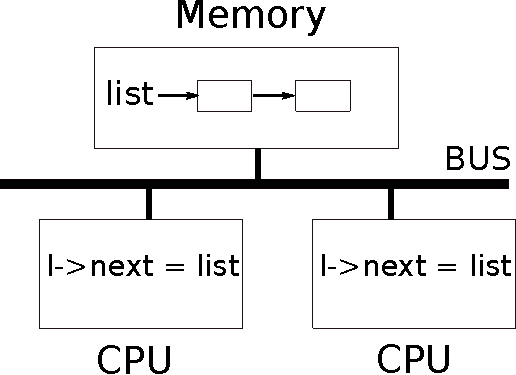
\includegraphics[scale=0.8]{fig/smp.pdf}
\caption{简化的SMP架构  }
\label{fig:smp}
\end{figure}     

作为我们为什么需要锁的一个例子,考虑两个带有退出子进程的进程
 两个不同 CPU 上的  {    \tt    wait   } 。  {    \tt    wait   }  释放子进程的内存。因此每个CPU,内核都会调用 {    \tt    kfree   } 来释放子进程的内存页面。内核分配器维护一个链表:   \lstinline{kalloc()}       \lineref{kernel/kalloc.c:/^kalloc/}    从空闲页列表中弹出一页内存,   \lstinline{kfree()}   
 \lineref{kernel/kalloc.c:/^kfree/}    将页面推送到空闲列表上。为了获得最佳性能,我们可能希望两个父进程的  {    \tt    kfree   }  能够并行执行,而不必等待另一个,但考虑到 xv6 的  {    \tt    kfree   }  实现,这是不正确的。  

图~\ref{fig:smp}   更详细地说明了该设置:空闲页面的链接列表位于由两个CPU共享的内存中,这两个CPU使用加载和存储指令来操作该列表。 (实际上,处理器有缓存,但从概念上讲,多处理器系统的行为就好像有一个共享内存一样。)如果没有并发请求,您可以实现列表    \lstinline{push}    操作,如下所示:
    \begin{lstlisting}[numbers=left,firstnumber=1]
    struct element {
      int data;
      struct element *next;
    };
    
    struct element *list = 0;
    
    void
    push(int data)
    {
      struct element *l;
   
      l = malloc(sizeof *l);
      l->data = data;
      l->next = list; (*@\label{line:next}@*)
      list = l;  (*@\label{line:list}@*)
   }
\end{lstlisting}     

   \begin{figure}[t]
\center
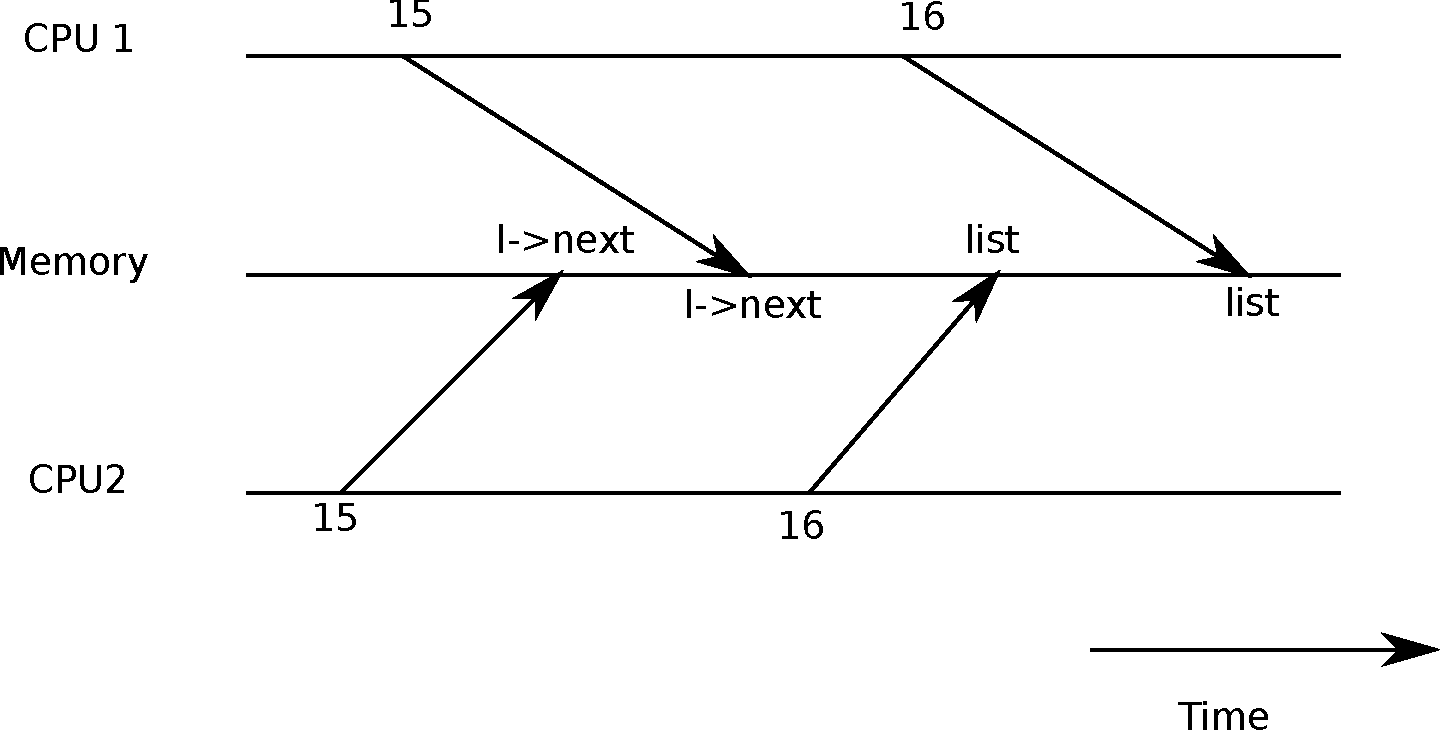
\includegraphics[scale=0.5]{fig/race.pdf}
\caption{竞争示例  }
\label{fig:race}
\end{figure}    如果单独执行,此实现是正确的。但是,如果同时执行多个副本,则代码不正确。如果有两个CPU执行
    \lstinline{push}    同时,两者都可能执行 line~\ref{line:next}    (如图~\ref{fig:smp}    所示),然后再执行 line~\ref{line:list}    ,这会导致错误的结果,如图~\ref{fig:race}    所示。然后会有twolist元素
    \lstinline{next}    设置为以前的值
    \lstinline{list}   。当两个任务分配到
    \lstinline{list}    发生在 ~\ref{line:list}    行,第二个将覆盖第一个;第一个赋值涉及的元素将丢失。  

行 ~\ref{line:list}    处丢失的更新是一个示例
    \indextext{race}    。竞争是一种同时访问内存位置且至少一次访问是写入的情况。竞争通常是错误的迹象,要么是更新丢失(如果访问是写入),要么是读取未完全更新的数据结构。竞争的结果取决于编译器生成的机器代码、所涉及的两个 CPU 的时序以及内存系统如何排序它们的内存操作,这可能会使竞争引起的错误难以重现和调试。例如,调试时添加打印语句
    \lstinline{push}    可能会改变执行的时间,足以使竞争消失。  

避免竞争的常用方法是使用锁。锁确保
    \indextext{mutual exclusion}    ,这样一次只有一个CPU可以执行以下敏感行
    \lstinline{push}    ;这使得上述情况变得不可能。上述代码的正确锁定版本仅添加了几行(以黄色突出显示):
    \begin{lstlisting}[numbers=left,firstnumber=6]
   struct element *list = 0;
   (*@\hl{struct lock listlock;}@*)
    	
   void
   push(int data)
   {
     struct element *l;
     l = malloc(sizeof *l); (*@\label{line:malloc}@*)
     l->data = data;
   
     (*@\hl{acquire( \& listlock);} @*)
     l->next = list;     (*@\label{line:next1}@*)
     list = l;           (*@\label{line:list1}@*)
     (*@\hl{release( \& listlock)}; @*)
   }
\end{lstlisting}    之间的指令序列
    \lstinline{acquire}    和
    \lstinline{release}    通常被称为
    \indextext{critical section}    。锁通常被认为是保护
    \lstinline{list}    。  

当我们说锁保护数据时,我们真正的意思是锁保护一些适用于数据的不变量集合。不变量是跨操作维护的数据结构的属性。通常,操作的正确行为取决于操作开始时不变量是否为真。该操作可能会暂时违反不变量,但必须在完成之前重新建立它们。例如,在链表情况下,不变量是
    \lstinline{list}    指向列表中的第一个元素,并且每个元素的
    \lstinline{next}    字段指向下一个元素。实施
    \lstinline{push}    暂时违反了这个不变量:在~\ref{line:next1}    行中,
    \lstinline{l}    指向下一个列表元素,但是
    \lstinline{list}    没有指向
    \lstinline{l}    尚未(在 ~\ref{line:list1}    行重新建立)。我们上面检查的竞争之所以发生,是因为第二个 CPU 执行了依赖于列表不变量的代码,而它们(暂时)被违反了。正确使用锁可以确保一次只有一个 CPU 可以对临界区中的数据结构进行操作,这样当数据结构的不变量不成立时,没有 CPU 会执行该数据结构操作。  

你可以把锁想象成
    \indextext{serializing}    并发关键部分,以便它们一次运行一个,从而保留不变量(假设关键部分单独正确)。您还可以将由同一锁保护的关键部分视为彼此之间的原子性,以便每个关键部分只能看到较早关键部分的完整更改集,而永远不会看到部分完成的更新。  

虽然锁对于正确性很有用,但它本质上限制了性能。例如,如果两个进程同时调用  {    \tt    kfree   } ,锁将序列化两个临界区,因此在不同的 CPU 上运行它们没有任何好处。如果多个进程同时想要相同的锁,则我们说多个进程    \indextext{conflict}    ,或者该锁经历    \indextext{contention}    。内核设计中的一个主要挑战是避免锁争用以追求并行性。 Xv6 几乎没有做到这一点,但复杂的内核专门组织了数据结构和算法来避免锁争用。在列表示例中,内核可以为每个 CPU 维护一个单独的空闲列表,并且仅在当前 CPU 的列表为空并且必须从另一个 CPU 窃取内存时才触及另一个 CPU 的空闲列表。其他用例可能需要更复杂的设计。  

锁的放置对于性能也很重要。例如,移动是正确的
 早些时候的    \lstinline{acquire}   
    \lstinline{push}    ,在行~\ref{line:malloc}    之前。但这可能会降低性能,因为随后的调用
    \lstinline{malloc}    将被序列化。下面的“使用锁”部分提供了一些关于插入位置的指南
    \lstinline{acquire}    和
    \lstinline{release}    调用。
    \section{代码: 锁  }    Xv6 有两种类型的锁:自旋锁和睡眠锁。我们将从自旋锁开始。 Xv6 将自旋锁表示为
    \indexcode{struct spinlock}   
    \lineref{kernel/spinlock.h:/struct.spinlock/}    。该结构中重要的字段是
    \lstinline{locked}    ,当锁可用时该字为零,而当锁被持有时该字为非零。从逻辑上讲,xv6 应该通过执行类似的代码来获取锁
    \begin{lstlisting}[numbers=left,firstnumber=21]
   void
   acquire(struct spinlock *lk) // does not work!
   {
     for(;;) {
       if(lk->locked == 0) {  (*@\label{line:testlocked}@*)
         lk->locked = 1;      (*@\label{line:assign}@*)
         break;
       }
     }
   }
\end{lstlisting}    不幸的是,此实现不能保证多处理器上的互斥。可能会发生两个 CPU 同时到达线 ~\ref{line:testlocked}    ,请参阅
    \lstinline{lk->locked}    为零,然后两者都通过执行 line~\ref{line:assign}    来获取锁。此时,两个不同的CPU持有锁,这违反了互斥性质。我们需要的是一种使    \ref{line:testlocked}    和    \ref{line:assign}    行作为
    \indextext{atomic}   (即不可分割的)步骤。  

由于锁被广泛使用,多核处理器通常提供实现原子版本的指令~\ref{line:testlocked}    和    \ref{line:assign}    。在 RISC-V 上,这条指令是
    \lstinline{amoswap r, a}    。
    \lstinline{amoswap}    读取内存地址  {    \tt    a   }  处的值,将寄存器  {    \tt    r   }  的内容写入该地址,并将读取到的值放入  {    \tt    r   }  中。也就是说,它交换了寄存器的内容和内存地址。它以原子方式执行此序列,使用特殊硬件来防止任何其他 CPU 使用读取和写入之间的内存地址。  

Xv6的
    \indexcode{acquire}   
    \lineref{kernel/spinlock.c:/^acquire/}    使用可移植 C 库调用
    \lstinline{__sync_lock_test_and_set}    ,归结为
    \lstinline{amoswap}    指令;返回值是旧的(交换的)内容
    \lstinline{lk->locked}    。这
    \lstinline{acquire}    函数将交换包装在循环中,重试(旋转)直到获得锁。每次迭代都会将一个交换为
    \lstinline{lk->locked}    并检查先前的值;如果先前的值为零,那么我们已经获得了锁,并且交换将被设置
    \lstinline{lk->locked}    比 1。如果前一个值是 1,则其他某个 CPU 持有该锁,并且我们以原子方式将 1 交换为
    \lstinline{lk->locked}    没有改变它的值。  

一旦获得锁,
    \lstinline{acquire}    记录获取锁的 CPU,以供调试。这
    \lstinline{lk->cpu}    字段受锁保护,并且只能在持有锁时更改。  

功能
    \indexcode{release}   
    \lineref{kernel/spinlock.c:/^release/}    与
    \lstinline{acquire}    :它清除
    \lstinline{lk->cpu}    字段,然后释放锁。从概念上讲,该版本只需要将零分配给
    \lstinline{lk->locked}    。 C 标准允许编译器使用多个存储指令实现赋值,因此 C 赋值对于并发代码来说可能是非原子的。反而,
    \lstinline{release}   使用C库函数
 执行原子赋值的    \lstinline{__sync_lock_release}   。该功能也归结为 RISC-V
    \lstinline{amoswap}    指令。
    \section{代码:使用锁  }    Xv6 在许多地方使用锁来避免竞争。如上所述,
    \lstinline{kalloc}   
    \lineref{kernel/kalloc.c:/^kalloc/}    和
    \lstinline{kfree}   
    \lineref{kernel/kalloc.c:/^kfree/}    就是一个很好的例子。尝试练习 1 和 2,看看如果这些函数忽略锁会发生什么。您可能会发现很难触发不正确的行为,这表明很难可靠地测试代码是否没有锁定错误和竞争。 Xv6 很可能有尚未被发现的种族。  

使用锁的一个困难部分是决定使用多少个锁以及每个锁应保护哪些数据和不变量。有一些基本原则。首先,只要一个 CPU 可以写入变量,同时另一个 CPU 可以读取或写入该变量,则应使用锁来防止两个操作重叠。其次,请记住锁保护不变量:如果不变量涉及多个内存位置,通常所有这些位置都需要由单个锁保护以确保不变量得到维护。  

上面的规则说明了何时需要锁,但没有提及何时不需要锁,并且不要锁太多对于效率很重要,因为锁会降低并行性。如果并行性不重要,那么可以安排只有一个线程而不用担心锁。简单的内核可以在多处理器上通过拥有一个锁来做到这一点,该锁必须在进入内核时获取并在退出内核时释放(尽管会阻塞系统调用,例如管道读取或
    \lstinline{wait}    会造成问题)。许多单处理器操作系统已使用这种方法转换为在多处理器上运行,有时称为“大内核锁”,但该方法牺牲了并行性:一次只有一个 CPU 可以在内核中执行。如果内核执行任何繁重的计算,那么使用更大的一组更细粒度的锁会更有效,以便内核可以同时在多个CPU上执行。  

作为粗粒度锁定的示例,xv6 的    \lstinline{kalloc.c}    分配器具有受单个锁保护的单个空闲列表。如果不同 CPU 上的多个进程尝试同时分配页面,则每个进程都必须通过在  {    \tt    acquire   }  中旋转来等待轮到它。旋转会浪费 CPU 时间,因为它不是有用的工作。如果锁争用浪费了很大一部分 CPU 时间,也许可以通过更改分配器设计来提高性能,使其具有多个空闲列表,每个列表都有自己的锁,以允许真正的并行分配。  

作为细粒度锁定的一个示例,xv6 对每个文件都有一个单独的锁,因此操作不同文件的进程通常可以继续执行而无需等待彼此的锁。如果希望允许进程同时写入同一文件的不同区域,则可以使文件锁定方案变得更加细粒度。最终,锁粒度决策需要由性能测量和复杂性考虑来驱动。  

后续章节在解释 xv6 的各个部分时,会提到 xv6 使用锁来处理并发的示例。作为预览,图~\ref{fig:locktable}    列出了 xv6 中的所有锁。  

   \begin{figure}[t]
\center
\begin{tabular}{ll}
{\bf Lock} & {\bf Description}  \\ 
\midrule bcache.lock & Protects allocation of block buffer cache entries  \\ cons.lock & Serializes access to console hardware, avoids intermixed output  \\ ftable.lock & Serializes allocation of a struct file in file table  \\ itable.lock & Protects allocation of in-memory inode entries  \\ vdisk\_lock & Serializes access to disk hardware and queue of DMA descriptors  \\ kmem.lock & Serializes allocation of memory  \\ log.lock & Serializes operations on the transaction log  \\ pipe's pi->lock & Serializes operations on each pipe  \\ pid\_lock & Serializes increments of next\_pid  \\ proc's p->lock & Serializes changes to process's state  \\ wait\_lock & Helps wait avoid lost wakeups  \\ tickslock & Serializes operations on the ticks counter  \\ inode's ip->lock & Serializes operations on each inode and its content  \\ buf's b->lock & Serializes operations on each block buffer  \\ 
\end{tabular}
\caption{锁定 xv6  }
\label{fig:locktable}
\end{figure}   
    \section{死锁和锁顺序  }    如果通过内核的代码路径必须同时持有多个锁,则所有代码路径以相同的顺序获取这些锁非常重要。如果不这样做,则存在    \indextext{deadlock}    的风险。假设有两条代码路径 inxv6 需要锁 A 和 B,但是代码路径 1 按照 Athen B 的顺序获取锁,而另一条路径则按照 B 然后 A 的顺序获取锁。假设线程 T1 执行代码路径 1 并获取锁 A,并且线程 T2 执行代码路径 2 并获取锁 B。接下来,T1 将尝试获取锁 B,T2 将尝试获取锁 A。这两种获取都会无限期地阻塞,因为在这两种情况下,另一个线程都持有所需的锁,并且不会释放它直到它获取返回。为了避免此类死锁,所有代码路径必须以相同的顺序获取锁。对全局锁获取顺序的需求意味着锁实际上是每个函数规范的一部分:调用者必须以导致按照商定的顺序获取锁的方式调用函数。  

Xv6 有许多长度为 2 的锁顺序链,涉及每个进程锁(每个进程中的锁)
    \lstinline{struct proc}    )由于这样的方式
    \lstinline{sleep}    有效(参见章节~\ref {CH:SCHED}    )。例如,
    \lstinline{consoleintr}   
    \lineref{kernel/console.c:/^consoleintr/}    是处理键入字符的中断例程。当换行符到达时,任何正在等待控制台输入的进程都应该被唤醒。去做这个,
    \lstinline{consoleintr}    成立
 通话时    \lstinline{cons.lock}   
    \indexcode{wakeup}    ,它获取等待进程的锁以唤醒它。因此,全局死锁避免锁顺序包括以下规则:
 必须在任何进程锁之前获取    \lstinline{cons.lock}   。文件系统代码包含 xv6 最长的锁链。例如,创建文件需要同时持有目录上的锁、新文件的 inode 上的锁、磁盘块缓冲区上的锁、磁盘驱动程序的    \lstinline{vdisk_lock}    和调用进程的    \lstinline{p->lock}    。为了避免死锁,文件系统代码始终按照上一句中提到的顺序获取锁。  

遵守全球避免僵局的秩序可能异常困难。有时,锁定顺序与逻辑程序结构冲突,例如,代码模块 M1 可能调用模块 M2,但锁定顺序要求先获取 M2 中的锁,然后再获取 M1 中的锁。有时,锁的身份事先并不知道,也许是因为必须持有一个锁才能发现下一个要获取的锁的身份。这种情况出现在文件系统中,因为它在路径名中查找连续的组件,并且在  {    \tt    wait   }  和  {    \tt    exit   }  的代码中,当它们搜索进程表以查找子进程时。最后,死锁的危险通常是对锁定方案的细粒度程度的限制,因为更多的锁通常意味着更多的死锁机会。避免死锁的需要通常是内核实现的一个主要因素。  

   \section{可重入锁  }     

使用    \indextext{re-entrant locks}   (也称为    \indextext{recursive locks}   )似乎可以避免一些死锁和锁排序挑战。这个想法是,如果锁被一个进程持有,并且该进程尝试再次获取锁,那么内核可以允许这样做(因为该进程已经拥有锁),而不是像 xv6 内核那样调用Panic。  

然而,事实证明,可重入锁使推理并发性变得更加困难:可重入锁打破了锁导致临界区相对于其他临界区是原子的直觉。考虑以下两个函数    \lstinline{f}    和
    \lstinline{g}   :  

   \begin{lstlisting}struct spinlock lock;int data = 0; // protected by lock

f() {
  acquire(&lock);
  if(data == 0){
    call_once();
    h();
    data = 1;
  }
  release(&lock);
}

g() {
  aquire(&lock);
  if(data == 0){
    call_once();
    data = 1;
  }
  release(&lock);
}
\end{lstlisting}     

看看这个代码片段,直觉是
    \lstinline{call_once}    将仅被调用一次:由    \lstinline{f}    或    \lstinline{g}    调用,但不能同时由两者调用。  

但是如果允许重入锁,并且    \lstinline{h}    恰好调用
    \lstinline{g}   、   \lstinline{call_once}   将被调用两次。  

如果不允许重入锁,则    \lstinline{h}    调用
    \lstinline{g}    会导致死锁,这也不是很好。但是,假设调用将是一个严重的错误
    \lstinline{call_once}    ,最好是死锁。内核开发人员将观察死锁(内核Panic),并可以修复代码以避免死锁,同时调用
    \lstinline{call_once}    两次可能会默默地导致难以追踪的错误。  

为此,xv6 使用了更容易理解的不可重入锁。然而,只要程序员牢记锁定规则,任何一种方法都可以发挥作用。如果 xv6 要使用重入锁,则必须修改    \lstinline{acquire}    才能注意到该锁当前由调用线程持有。还必须向 struct spinlock 添加嵌套获取的计数,其风格与    \lstinline{push_off}    类似,这将在接下来讨论。  

   \section{锁和中断处理程序  }   
    \label{s:lockinter}    一些 xv6 自旋锁保护线程和中断处理程序使用的数据。例如,
    \lstinline{clockintr}    定时器中断处理程序可能会增加
    \indexcode{ticks}   
    \lineref{kernel/trap.c:/^clockintr/}    大约在内核线程读取的同时
    \lstinline{ticks}    中
    \indexcode{sys_sleep}   
    \lineref{kernel/sysproc.c:/ticks0.=.ticks/}   。锁
    \indexcode{tickslock}    序列化这两个访问。  

自旋锁和中断的相互作用会带来潜在的危险。假如
    \indexcode{sys_sleep}    持有
    \indexcode{tickslock}   ,其CPU被定时器中断中断。
    \lstinline{clockintr}    会尝试获取
    \lstinline{tickslock}    ,看到它被持有,并等待它被释放。在这个情况下,
    \lstinline{tickslock}    永远不会被释放:仅
    \lstinline{sys_sleep}   可以释放它,但是
    \lstinline{sys_sleep}    将不会继续运行,直到
    \lstinline{clockintr}    返回。因此,CPU 将发生死锁,并且任何需要任一锁的代码也将冻结。  

为了避免这种情况,如果中断处理程序使用自旋锁,则 CPU 绝不能在启用中断的情况下持有该锁。 Xv6 更加保守:当 CPU 获取任意锁时,xv6 始终禁用该 CPU 上的中断。中断可能仍会发生在其他 CPU 上,因此中断的
    \lstinline{acquire}   可以等待线程释放自旋锁;只是不在同一个CPU上。  

当 CPU 没有自旋锁时,Xv6 重新启用中断;它必须做一些簿记来处理嵌套的关键部分。
    \lstinline{acquire}    次调用
    \indexcode{push_off}   
    \lineref{kernel/spinlock.c:/^push_off/}    和
    \lstinline{release}    调用
    \indexcode{pop_off}   
    \lineref{kernel/spinlock.c:/^pop_off/}    跟踪当前 CPU 上锁的嵌套级别。当该计数达到零时,
    \lstinline{pop_off}    恢复最外层临界区开始处存在的中断使能状态。这
    \lstinline{intr_off}    和
    \lstinline{intr_on}    函数执行 RISC-V 指令来分别禁用和启用中断。  

重要的是
    \indexcode{acquire}    调用
    \lstinline{push_off}    严格在设置之前
    \lstinline{lk->locked}   
    \lineref{kernel/spinlock.c:/sync_lock_test_and_set/}    。如果两者颠倒,则在启用中断的情况下保持锁定时会出现一个短暂的窗口,不幸的是定时中断将使系统死锁。同样,重要的是
    \indexcode{release}    调用
    \indexcode{pop_off}    仅在释放锁后
    \lineref{kernel/spinlock.c:/sync_lock_release/}    。
    \section{指令和内存排序  }     

人们很自然地认为程序是按照源代码语句出现的顺序执行的。对于单线程代码来说,这是一个合理的心理模型,但当多个线程通过共享内存交互时,这是不正确的~    \cite{riscv:user,boehm04}    。原因之一是编译器发出加载和存储指令的顺序与源代码所暗示的顺序不同,并且可能完全省略它们(例如通过在寄存器中缓存数据)。另一个原因是CPU可能会乱序执行指令以提高性能。例如,CPU 可能会注意到指令 A 和 B 的串行序列中并不相互依赖。 CPU 可能会首先启动指令 B,要么是因为其输入在 A 的输入之前准备好,要么是为了重叠执行 A 和 B。  

作为可能出错的示例,在这段代码中
    \lstinline{push}    ,如果编译器或 CPU 将对应于 line~\ref{line:next2}    的存储移动到该行之后的点,那将是一场灾难
    \lstinline{release}   上线~\ref{line:release}   :
    \begin{lstlisting}[numbers=left,firstnumber=1]
      l = malloc(sizeof *l);
      l->data = data;
      acquire(&listlock);
      l->next = list;   (*@\label{line:next2}@*)
      list = l;      
      release(&listlock);  (*@\label{line:release}@*)
\end{lstlisting}    如果发生这样的重新排序,将会出现一个窗口,在此期间另一个 CPU 可以获取锁并观察更新的结果
    \lstinline{list}    ,但看到一个未初始化的
    \lstinline{list->next}    。  

好消息是,编译器和 CPU 遵循一组称为    \indextext{memory model}    的规则,并提供一些原语来帮助程序员控制重新排序,从而帮助并发程序员。  

为了告诉硬件和编译器不要重新排序,xv6 使用
 两者均    \lstinline{__sync_synchronize()}   
    \lstinline{acquire}       \lineref{kernel/spinlock.c:/^acquire/}    和
    \lstinline{release}       \lineref{kernel/spinlock.c:/^release/}    。
    \lstinline{__sync_synchronize()}    是    \indextext{memory barrier}    :它告诉编译器和 CPU 不要跨障碍重新排序加载或存储。 xv6 中的障碍
    \lstinline{acquire}    和
    \lstinline{release}    在几乎所有重要的情况下都强制执行顺序,因为 xv6 在共享数据的访问周围使用锁。第~\ref{CH:LOCK2}    章讨论了一些例外情况。
    \section{睡眠锁  }     

有时xv6需要长时间持有锁。例如,文件系统(Chapter~\ref{CH:FS}   )在磁盘上读取和写入文件内容时保持文件锁定,这些磁盘操作可能需要数十毫秒。如果另一个进程想要获取自旋锁,那么长时间持有该自旋锁会导致浪费,因为获取进程会在自旋时长时间浪费 CPU。自旋锁的另一个缺点是进程在保留自旋锁的同时无法让出 CPU。我们希望这样做,以便其他进程可以在拥有锁的进程等待磁盘时使用 CPU。持有自旋锁时让出是非法的,因为如果第二个线程随后尝试获取自旋锁,可能会导致死锁;由于  {    \tt    acquire   }  不让出 CPU,第二个线程的自旋可能会阻止第一个线程运行并释放锁。在持有锁时让出也会违反在持有自旋锁时中断必须关闭的要求。因此,我们需要一种在等待获取时让出 CPU,并在持有锁时允许让出(和中断)的锁。  

Xv6 以以下形式提供此类锁
    \indextext{sleep-locks}    。
    \lstinline{acquiresleep}   
    \lineref{kernel/sleeplock.c}{22}    在等待时使用 CPU,使用的技术将在第    \ref{CH:SCHED}    章中解释。在较高级别上,睡眠锁具有
 由自旋锁保护的    \lstinline{locked}    字段,以及
    \lstinline{acquiresleep}    '调用
    \lstinline{sleep}    以原子方式让出 CPU 并释放自旋锁。结果是其他线程可以执行 while
    \lstinline{acquiresleep}    等待。  

由于睡眠锁使中断保持启用状态,因此它们不能在中断处理程序中使用。因为
    \lstinline{acquiresleep}    可能会占用 CPU,睡眠锁不能在自旋锁关键部分内使用(尽管自旋锁可以在睡眠锁关键部分内使用)。  

自旋锁最适合短临界区,因为等待它们会浪费 CPU 时间;睡眠锁非常适合长时间操作。
    \section{真实世界  }    尽管对并发原语和并行性进行了多年的研究,但使用锁进行编程仍然具有挑战性。通常最好在同步队列等更高级别的构造中隐藏锁,尽管 xv6 没有这样做。如果您使用锁进行编程,那么明智的做法是使用尝试识别竞争的工具,因为很容易错过需要锁的不变量。  

大多数操作系统支持 POSIX 线程 (Pthreads),它允许用户进程在不同的 CPU 上同时运行多个线程。 Pthreads 支持用户级锁、屏障等。Pthreads 还允许程序员有选择地指定锁应该是可重入的。  

在用户级别支持 Pthreads 需要操作系统的支持。例如,如果一个 pthread 在系统调用中阻塞,则同一进程的另一个 pthread 应该能够在该 CPU 上运行。作为另一个示例,如果 pthread 更改其进程的地址空间(例如,映射或取消映射内存),则内核必须安排运行同一进程的线程的其他 CPU 更新其硬件页表以反映地址空间中的更改。  

可以在没有原子指令的情况下实现锁~    \cite{lamport:bakery}    ,但它很昂贵,并且大多数操作系统都使用原子指令。  

如果许多 CPU 尝试同时获取相同的锁,那么锁的成本可能会很高。如果一个 CPU 在其本地缓存中缓存了一个锁,而另一个 CPU 必须获取该锁,则更新持有该锁的缓存行的原子指令必须将该行从一个 CPU 的缓存移动到另一个 CPU 的缓存,并且可能会使任何其他副本无效缓存行的。从另一个 CPU 的高速缓存中获取高速缓存行的成本可能比从本地高速缓存中获取高速缓存行的成本高出几个数量级。  

为了避免与锁相关的开销,许多操作系统使用无锁数据结构和算法~    \cite{herlihy:art,mckenney:rcuusage}    。例如,可以实现像本章开头那样的链表,在列表搜索期间不需要锁,并且需要一条原子指令在列表中插入一项。然而,无锁编程比锁编程更复杂。例如,我们必须担心指令和内存的重新排序。使用锁编程已经很困难,因此 xv6 避免了无锁编程的额外复杂性。
    \section{练习  }     

   \begin{enumerate}

 
   \item   注释掉以下调用
    \lstinline{acquire}    和
    \lstinline{release}    中
    \lstinline{kalloc}   
    \lineref{kernel/kalloc.c:/^kalloc/}    。这似乎应该会导致调用的内核代码出现问题
    \lstinline{kalloc}    ;您预计会看到什么症状?当您运行 xv6 时,您是否看到这些症状?跑步的时候怎么样
    \lstinline{usertests}   ?如果您没有发现问题,为什么不呢?看看是否可以通过将虚拟循环插入到关键部分来引发问题
    \lstinline{kalloc}    。   \item   假设您注释掉了锁定
    \lstinline{kfree}   (恢复锁定后
    \lstinline{kalloc}   )。现在可能会出现什么问题?是否缺少锁
    \lstinline{kfree}    的危害性比
    \lstinline{kalloc}   ?   \item   如果两个CPU调用
    \lstinline{kalloc}    同时,一个必须等待另一个,这对性能不利。调整
    \lstinline{kalloc.c}    具有更多并行性,以便同时调用
 来自不同CPU的   \lstinline{kalloc}   可以继续进行而无需互相等待。   \item   使用大多数操作系统都支持的 POSIX 线程编写并行程序。例如,实现一个并行哈希表并测量放入/获取的数量是否随着核心数量的增加而变化。   \item   在 xv6 中实现 Pthread 的子集。即实现一个用户级线程库,使得一个用户进程可以有1个以上的线程,并安排这些线程可以在不同的CPU上并行运行。提出一种设计,可以正确处理线程进行阻塞系统调用并更改其共享地址空间。  \end{enumerate}     


   
    
\documentclass[UTF8]{article}
\usepackage{xeCJK}
\usepackage{amsmath,amssymb}
\begin{document}

   \chapter{Scheduling}   
    \label{CH:SCHED}     

任何操作系统运行的进程数都可能多于计算机的 CPU 数,因此需要制定计划来在进程之间分时共享 CPU。理想情况下,共享对用户进程是透明的。一种常见的方法是通过以下方式为每个进程提供它拥有自己的虚拟 CPU 的错觉:
    \indextext{multiplexing}    将进程转移到硬件 CPU 上。本章解释 xv6 如何实现这种多路复用。
    \section{多路复用  }     

Xv6 通过在两种情况下将每个 CPU 从一个进程切换到另一个进程来进行多路复用。首先是xv6
    \lstinline{sleep}    和
    \lstinline{wakeup}    机制在进程等待设备或管道 I/O 完成、等待子进程退出或等待进程时切换
    \lstinline{sleep}    系统调用。其次,xv6 定期强制切换以应对长时间计算而不休眠的进程。这种多路复用创建了每个进程都有自己的 CPU 的假象,就像 xv6 使用内存分配器和硬件页表来创建每个进程都有自己的内存的假象一样。  

实施多路复用带来了一些挑战。首先,如何从一个进程切换到另一个进程?虽然上下文切换的想法很简单,但实现是 xv6 中一些最不透明的代码。其次,如何以对用户进程透明的方式强制切换? Xv6 使用标准技术,其中硬件定时器的中断驱动上下文切换。第三,所有 CPU 在同一共享进程集之间切换,并且需要一个锁定计划来避免竞争。第四,进程退出时必须释放进程的内存和其他资源,但它本身无法完成所有这些操作,因为(例如)它无法在仍在使用自己的内核堆栈时释放它。第五,多核机器的每个核心必须记住它正在执行哪个进程,以便系统调用影响正确进程的内核状态。最后,   \lstinline{sleep}   和   \lstinline{wakeup}   允许进程放弃CPU并等待被另一个进程或中断唤醒。需要小心避免导致唤醒通知丢失的竞争。 Xv6 试图尽可能简单地解决这些问题,但生成的代码仍然很棘手。
    \section{代码:上下文切换  }     

   \begin{figure}[t]
\center
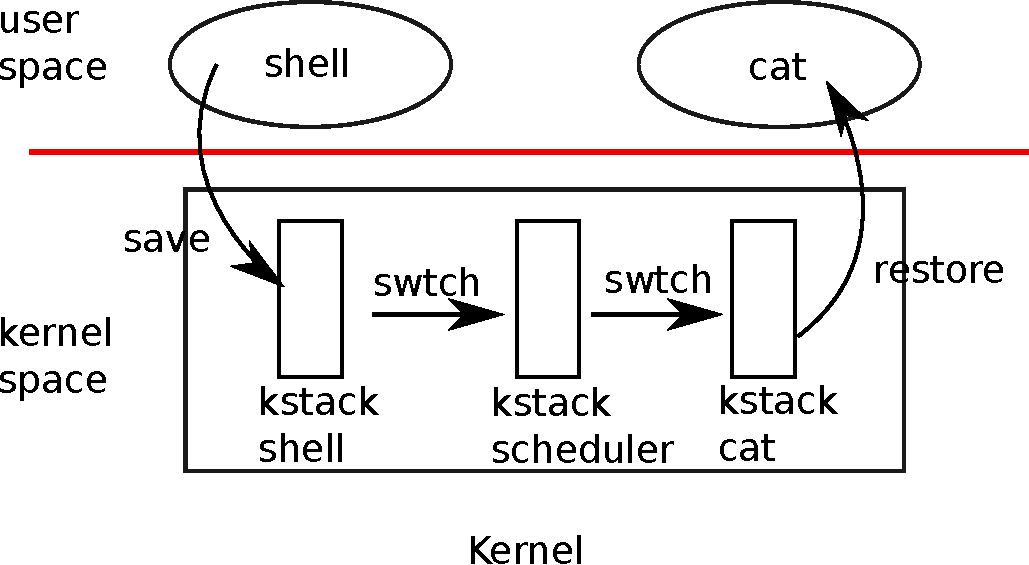
\includegraphics[scale=0.5]{fig/switch.pdf}
\caption{从一个用户进程切换到另一个用户进程。在此示例中,xv6 使用一个 CPU(因此也有一个调度程序线程)运行。  }
\label{fig:switch}
\end{figure}     

图〜   \ref{fig:switch}   概述了从一个用户进程切换到另一个用户进程所涉及的步骤:用户内核转换(系统调用或中断)到旧进程的内核线程,上下文切换到当前CPU的调度程序线程,上下文切换到新进程的内核线程,并返回用户级进程的陷阱。 xv6 调度程序为每个 CPU 有一个专用线程(保存的寄存器和堆栈),因为调度程序在旧进程的内核堆栈上执行是不安全的:其他一些核心可能会唤醒该进程并运行它,使用相同的线程将是一场灾难堆叠在两个不同的核心上。在本节中,我们将研究在内核线程和调度程序线程之间切换的机制。  

从一个线程切换到另一个线程涉及保存旧线程的CPU寄存器,并恢复新线程先前保存的寄存器;堆栈指针和程序计数器的保存和恢复意味着CPU将切换堆栈并切换正在执行的代码。  

功能
    \indexcode{swtch}    执行内核线程切换的保存和恢复。
    \lstinline{swtch}    不直接了解线程;它只是保存和恢复 32 个 RISC-V 寄存器组,称为
    \indextext{contexts}    。当进程需要放弃CPU时,进程的内核线程会调用
    \lstinline{swtch}    保存自己的上下文并返回到调度程序上下文。每个上下文都包含在一个
    \lstinline{struct}   
    \lstinline{context}   
    \lineref{kernel/proc.h:/^struct.context/}    ,本身包含在进程的
    \lstinline{struct proc}    或 CPU 的
    \lstinline{struct cpu}    。
    \lstinline{swtch}    有两个参数:
    \indexcode{struct context}   
    \lstinline{*old}    和
    \lstinline{struct}   
    \lstinline{context}   
    \lstinline{*new}    。它将当前寄存器保存在
    \lstinline{old}    ,加载寄存器
    \lstinline{new}    ,然后返回。  

让我们遵循一个流程
    \lstinline{swtch}    进入调度程序。我们在 Chapter~    \ref{CH:TRAP}    中看到,中断结束时的一种可能性是
    \indexcode{usertrap}    调用
    \indexcode{yield}    。
    \lstinline{yield}   依次调用
    \indexcode{sched}    ,它调用
    \indexcode{swtch}    将当前上下文保存在
    \lstinline{p->context}    并切换到先前保存的调度程序上下文
    \indexcode{cpu->context}   
    \lineref{kernel/proc.c:/swtch..p/}    。  

   \lstinline{swtch}   
    \lineref{kernel/swtch.S:/swtch/}    仅保存被调用者保存的寄存器;C 编译器在调用者中生成代码以将调用者保存的寄存器保存在堆栈上。
    \lstinline{swtch}    知道每个寄存器字段的偏移量
    \lstinline{struct context}    。它不保存程序计数器。反而,
    \lstinline{swtch}    保存
    \lstinline{ra}   寄存器,保存返回地址
    \lstinline{swtch}    被调用。现在
    \lstinline{swtch}    从新上下文中恢复寄存器,该上下文保存了先前保存的寄存器值
    \lstinline{swtch}    。什么时候
    \lstinline{swtch}   返回,它返回到恢复后的指令所指向的
    \lstinline{ra}    寄存器,即新线程之前调用    \lstinline{swtch}    的指令。此外,它返回新线程的堆栈,因为那是恢复的    \lstinline{sp}    所指向的位置。  

在我们的例子中,
 已调用    \indexcode{sched}   
 要切换到的    \indexcode{swtch}   
    \indexcode{cpu->context}    ,每 CPU 调度程序上下文。该上下文是在过去的某个时刻保存的
    \lstinline{scheduler}    已调用
    \lstinline{swtch}   
    \lineref{kernel/proc.c:/swtch.&c/}    切换到现在放弃 CPU 的进程。当。。。的时候
    \indexcode{swtch}   我们一直在追踪退货,它没有退货
    \lstinline{sched}    但
    \indexcode{scheduler}    ,当前CPU调度程序堆栈中的堆栈指针。
    \section{代码:调度  }     

最后一部分着眼于底层细节
    \indexcode{swtch}    ;现在我们来看
    \lstinline{swtch}    作为给定并检查通过调度程序从一个进程的内核线程切换到另一个进程。调度程序以每个 CPU 一个特殊线程的形式存在,每个线程运行
    \lstinline{scheduler}    函数。该函数负责选择接下来运行哪个进程。想要放弃CPU的进程必须获得自己的进程锁
    \indexcode{p->lock}    ,释放它持有的任何其他锁,更新自己的状态(    \lstinline{p->state}    ),然后调用
    \indexcode{sched}    。您可以在中看到此序列
    \lstinline{yield}   
    \lineref{kernel/proc.c:/^yield/}    ,
    \texttt{sleep}    和
    \texttt{exit}    。
    \lstinline{sched}    仔细检查其中一些要求
    \linerefs{kernel/proc.c:/if..holding/,/running/}    然后检查一个含义:由于持有锁,因此应该禁用中断。最后,
    \indexcode{sched}    调用
    \indexcode{swtch}    将当前上下文保存在
    \lstinline{p->context}    并切换到调度程序上下文
    \indexcode{cpu->context}    。
    \lstinline{swtch}    在调度程序的堆栈上返回
    \indexcode{scheduler}    的
    \lstinline{swtch}    已返回
    \lineref{kernel/proc.c:/swtch.*contex.*contex/}    。调度程序继续其
    \lstinline{for}   循环,找到要运行的进程,切换到它,然后重复循环。  

我们刚刚看到 xv6 成立
    \indexcode{p->lock}    跨调用
    \lstinline{swtch}    :调用者
    \indexcode{swtch}    必须已经持有该锁,并且该锁的控制权将传递给切换到的代码。这种约定对于锁来说是不常见的。通常,获取锁的线程也负责释放锁,这使得更容易推断正确性。对于上下文切换,有必要打破这个约定,因为
    \indexcode{p->lock}    保护进程的不变量
    \lstinline{state}    和
 执行时不正确的    \lstinline{context}    字段
    \lstinline{swtch}    。一个可能出现的问题的例子
    \lstinline{p->lock}    期间未举行
    \indexcode{swtch}   :不同的CPU可能决定在之后运行该进程
    \indexcode{yield}    已将其状态设置为
    \lstinline{RUNNABLE}    ,但之前
    \lstinline{swtch}    导致它停止使用自己的内核堆栈。结果将是两个 CPU 运行在同一个堆栈上,这会导致混乱。  

内核线程放弃其 CPU 的唯一地方是
    \lstinline{sched}    ,它总是切换到    \lstinline{scheduler}    中的同一位置,该位置(几乎)总是切换到先前调用的某个内核线程
    \lstinline{sched}    。因此,如果要打印出 xv6 切换线程的行号,就会观察到以下简单模式:
    \lineref{kernel/proc.c:/swtch..c/}    ,
    \lineref{kernel/proc.c:/swtch..p/}    ,
    \lineref{kernel/proc.c:/swtch..c/}    ,
    \lineref{kernel/proc.c:/swtch..p/}    等。故意通过线程切换相互转移控制的过程有时被称为
    \indextext{coroutines}   ;在这个例子中,
    \indexcode{sched}    和
    \indexcode{scheduler}    是彼此的协同例程。  

有一种情况,当调度程序调用
    \indexcode{swtch}    没有最终出现在
    \indexcode{sched}    。
    \lstinline{allocproc}    将新进程的上下文    \lstinline{ra}    寄存器设置为
    \indexcode{forkret}   
    \lineref{kernel/proc.c:/^forkret/}    ,以便其第一个    \lstinline{swtch}    “返回”到该函数的开头。
    \lstinline{forkret}    的存在是为了释放
    \indexcode{p->lock}    ;否则,由于新进程需要返回用户空间,就像从    \lstinline{fork}    返回一样,因此它可以从
    \lstinline{usertrapret}    。  

   \lstinline{scheduler}   
    \lineref{kernel/proc.c:/^scheduler/}    运行一个循环:找到一个要运行的进程,运行它直到它产生,重复。调度程序在进程表上循环查找可运行的进程,该进程具有
    \lstinline{p->state}   
    \lstinline{==}   
    \lstinline{RUNNABLE}    。一旦找到进程,它就会设置每个 CPU 的当前进程变量
    \lstinline{c->proc}    ,将进程标记为
    \lstinline{RUNNING}    ,然后调用
    \indexcode{swtch}    开始运行它
    \linerefs{kernel/proc.c:/Switch.to/,/swtch/}    。  

考虑调度代码结构的一种方法是,它对每个进程强制执行一组不变量,并保持
 每当这些不变量不成立时,   \indexcode{p->lock}   。一个不变量是,如果一个进程是
    \lstinline{RUNNING}    ,定时器中断
    \indexcode{yield}    必须能够安全地从进程切换;这意味着 CPU 寄存器必须保存进程的寄存器值(即
    \lstinline{swtch}    尚未将它们移至
    \lstinline{context}    ),以及
    \lstinline{c->proc}    必须引用该进程。另一个不变量是,如果一个进程
    \indexcode{RUNNABLE}    ,对于空闲 CPU 来说必须是安全的
    \indexcode{scheduler}    运行它;这意味着
    \indexcode{p->context}    必须保存进程的寄存器(即,它们实际上不在真实寄存器中),没有 CPU 在进程的内核堆栈上执行,并且没有 CPU
    \lstinline{c->proc}    指的是进程。观察到这些属性通常不正确,而
    \lstinline{p->lock}    被保持。  

保持上述不变量就是xv6经常获取的原因
    \indexcode{p->lock}    在一个线程中并在另一个线程中释放它,例如在
    \lstinline{yield}    并发布于
    \lstinline{scheduler}    。一旦    \lstinline{yield}    开始修改正在运行的进程的状态以使其
    \lstinline{RUNNABLE}    ,锁必须保持保持状态,直到不变量恢复:最早正确的释放点是在
    \lstinline{scheduler}   (在其自己的堆栈上运行)清除
    \lstinline{c->proc}    。同样,有一次
    \lstinline{scheduler}    开始将    \lstinline{RUNNABLE}    进程转换为
    \lstinline{RUNNING}    ,直到内核线程完全运行后(在
    \lstinline{swtch}    ,例如
    \lstinline{yield}    )。
    \section{代码:mycpu 和 myproc  }     

Xv6 通常需要一个指向当前进程的    \lstinline{proc}    结构的指针。在单处理器上,可以有一个指向当前    \lstinline{proc}    的全局变量。这在多核机器上不起作用,因为每个核心执行不同的进程。解决这个问题的方法是利用每个内核都有自己的寄存器组的事实;我们可以使用这些寄存器之一来帮助查找每个核心的信息。  

Xv6 保持
 每个 CPU 的    \indexcode{struct cpu}   
    \lineref{kernel/proc.h:/^struct.cpu/}    记录当前在该 CPU 上运行的进程(如果有)、为 CPU 调度程序线程保存的寄存器以及管理中断禁用所需的嵌套自旋锁的计数。功能
    \indexcode{mycpu}   
    \lineref{kernel/proc.c:/^mycpu/}    返回指向当前 CPU 的指针
    \lstinline{struct cpu}    。 RISC-V 对其 CPU 进行编号,给出每个    \indextext{hartid}    。 Xv6 确保每个 CPU 的 Hartid 在内核中存储在该 CPU 的    \lstinline{tp}    寄存器中。这允许
    \lstinline{mycpu}    使用    \lstinline{tp}    索引    \lstinline{cpu}    结构数组以找到正确的结构。  

确保CPU的   \lstinline{tp}   始终保存CPU的shartid有点复杂。    \lstinline{start}    在 CPU 启动序列的早期设置    \lstinline{tp}    寄存器,同时仍处于机器模式
    \lineref{kernel/start.c:/w_tp/}    。
    \lstinline{usertrapret}    将    \lstinline{tp}    保存在 Trampolinepage 中,因为用户进程可能会修改    \lstinline{tp}    。最后,   \lstinline{uservec}    恢复从用户空间进入内核时保存的    \lstinline{tp}   
    \lineref{kernel/trampoline.S:/make tp hold/}    。编译器保证永远不会使用    \lstinline{tp}    寄存器。如果xv6可以在需要时向RISC-V硬件询问当前的hartid,那就更方便了,但RISC-V仅在机器模式下允许,在管理模式下不允许。  

返回值
    \lstinline{cpuid}    和
    \lstinline{mycpu}    很脆弱:如果计时器中断并导致线程屈服,然后移动到不同的 CPU,则先前返回的值将不再正确。为了避免这个问题,xv6要求调用者禁用中断,并且只有在使用完返回的值后才启用它们
    \lstinline{struct cpu}    。  

功能
    \indexcode{myproc}   
    \lineref{kernel/proc.c:/^myproc/}    返回
    \lstinline{struct proc}    当前 CPU 上运行的进程的指针。
    \lstinline{myproc}    禁用中断,调用
    \lstinline{mycpu}   ,从内存中获取当前进程指针(   \lstinline{c->proc}   )
    \lstinline{struct cpu}   ,然后使能中断。返回值
 即使启用了中断,   \lstinline{myproc}    也可以安全使用:如果定时器中断将调用进程移至不同的 CPU,则其
    \lstinline{struct proc}    指针将保持不变。
    \section{睡眠和唤醒  }   
    \label{sec:sleep}     

调度和锁有助于向另一个线程隐藏一个线程的操作,但我们还需要帮助线程有意交互的抽象。例如,xv6 中管道的读取器可能需要等待写入进程产生数据;父进程对    \lstinline{wait}    的调用可能需要等待子进程退出;等等。而读取磁盘的进程需要等待磁盘硬件完成读取。 xv6 内核在这些情况(以及许多其他情况)中使用称为睡眠和唤醒的机制。睡眠允许内核线程等待特定事件;另一个线程可以调用wakeup来指示等待事件的线程应该恢复。睡眠和唤醒通常称为
    \indextext{sequence coordination}    或
    \indextext{conditional synchronization}    机制。  

睡眠和唤醒提供了相对低级的同步接口。为了激发它们在 xv6 中的工作方式,我们将使用它们构建一个称为    \indextext{semaphore}    ~    \cite{dijkstra65}    的更高级别同步机制,用于协调生产者和消费者(xv6 不使用信号量)。信号量维护计数并提供两个操作。 “V”操作(对于生产者)增加计数。 “P”操作(对于消费者)等待计数非零,然后将其递减并返回。如果只有一个生产者线程和一个消费者线程,并且它们在不同的 CPU 上执行,并且编译器没有过度优化,那么这种实现将是正确的:
    \begin{lstlisting}[numbers=left,firstnumber=100]
  struct semaphore {
    struct spinlock lock;
    int count;
  };

  void
  V(struct semaphore *s)
  {
     acquire(&s->lock);
     s->count += 1;
     release(&s->lock);
  }

  void
  P(struct semaphore *s)
  {
     while(s->count == 0)
       ;
     acquire(&s->lock);
     s->count -= 1;
     release(&s->lock);
  }
\end{lstlisting}     

上面的实现是昂贵的。如果生产者很少行动,消费者就会把大部分时间花在旋转上。
    \lstinline{while}    循环希望得到非零计数。消费者的 CPU 可能会找到比
    \indextext{busy waiting}    反复
    \indextext{polling}   
    \lstinline{s->count}    。避免忙等待需要一种方法让消费者让出 CPU 并仅在之后恢复
    \lstinline{V}    增加计数。  

这是朝着这个方向迈出的一步,尽管我们将看到这还不够。让我们想象一下一对电话,
    \indexcode{sleep}    和
    \indexcode{wakeup}    ,工作原理如下。
    \lstinline{sleep(chan)}    在任意值上休眠
    \indexcode{chan}    ,称为
    \indextext{wait channel}    。
    \lstinline{sleep}    将调用进程置于睡眠状态,释放 CPU 进行其他工作。
    \lstinline{wakeup(chan)}    唤醒所有休眠的进程
    \lstinline{chan}   (如果有),导致他们
    \lstinline{sleep}    调用返回。如果没有进程在等待
    \lstinline{chan}    ,
    \lstinline{wakeup}    不执行任何操作。我们可以改变信号量的实现来使用
    \lstinline{sleep}    和
    \lstinline{wakeup}   (更改以黄色突出显示):
    \begin{lstlisting}[numbers=left,firstnumber=200]
  void
  V(struct semaphore *s)
  {
     acquire(&s->lock);
     s->count += 1;
     (*@\hl{wakeup(s);}@*)
     release(&s->lock);
  }
  
  void
  P(struct semaphore *s)
  {
    while(s->count == 0)    (*@\label{line:test}@*)
      (*@\hl{sleep(s);}@*)  (*@\label{line:sleep}@*)
    acquire(&s->lock);
    s->count -= 1;
    release(&s->lock);
  }
\end{lstlisting}     

   \lstinline{P}    现在放弃 CPU 而不是旋转,这很好。然而,事实证明设计起来并不简单
    \lstinline{sleep}    和
 具有此接口的    \lstinline{wakeup}    不会遇到所谓的    \indextext{lost wake-up}    问题。假设
    \lstinline{P}    发现
    \lstinline{s->count}   
    \lstinline{==}   
    \lstinline{0}    上线~    \ref{line:test}    。尽管
    \lstinline{P}    位于 ~    \ref{line:test}    和 ~    \ref{line:sleep}    行之间,
    \lstinline{V}    在另一个 CPU 上运行:它发生了变化
    \lstinline{s->count}    为非零并调用
    \lstinline{wakeup}    ,它发现没有进程处于睡眠状态,因此不执行任何操作。现在
    \lstinline{P}    继续在 line~    \ref{line:sleep}    处执行:它调用
    \lstinline{sleep}    并进入睡眠状态。这会导致一个问题:
    \lstinline{P}    正在休眠,等待已发生的    \lstinline{V}    调用。除非我们运气好,制片人打电话来
 再次    \lstinline{V}   ,即使计数不为零,消费者也将永远等待。  

这个问题的根源在于不变式
    \lstinline{P}    仅在以下情况下休眠
    \lstinline{s->count}   
    \lstinline{==}   
    \lstinline{0}    被违反
    \lstinline{V}    在错误的时刻运行。保护不变量的错误方法是将锁获取(下面以黄色突出显示)移至
    \lstinline{P}    以便其对计数的检查和对    \lstinline{sleep}    的调用是原子的:
    \begin{lstlisting}[numbers=left,firstnumber=300]
  void
  V(struct semaphore *s)
  {
    acquire(&s->lock);
    s->count += 1;
    wakeup(s);
    release(&s->lock);
  }
  
  void
  P(struct semaphore *s)
  {
    (*@\hl{acquire( \& s->lock);}@*)
    while(s->count == 0)    (*@\label{line:test1}@*)
      sleep(s);             (*@\label{line:sleep1}@*)
    s->count -= 1;
    release(&s->lock);
  }
\end{lstlisting}    人们可能希望这个版本
    \lstinline{P}    将避免丢失唤醒,因为锁会阻止
    \lstinline{V}    在 ~    \ref{line:test1}    和 ~    \ref{line:sleep1}    行之间执行。它确实做到了这一点,但也陷入了僵局:
    \lstinline{P}    在休眠时持有锁,因此    \lstinline{V}    将永远阻塞等待锁。  

我们将通过更改来修复前面的方案
    \lstinline{sleep}    'sinterface:调用者必须将    \indextext{condition lock}    传递给
    \lstinline{sleep}    因此它可以在调用进程被标记为睡眠并在睡眠通道上等待后释放锁。锁会强制并发
    \lstinline{V}    等待    \lstinline{P}    完成使其自身进入睡眠状态,以便
    \lstinline{wakeup}   将找到正在睡眠的消费者并将其唤醒。一旦消费者再次醒来
    \indexcode{sleep}    在返回之前重新获取锁。我们新的正确睡眠/唤醒方案可按如下方式使用(更改以黄色突出显示):
    \begin{lstlisting}[numbers=left,firstnumber=400]
  void
  V(struct semaphore *s)
  {
    acquire(&s->lock);
    s->count += 1;
    wakeup(s);
    release(&s->lock);
  }

  void
  P(struct semaphore *s)
  {
    acquire(&s->lock);
    while(s->count == 0)
       (*@\hl{sleep(s,  \& s->lock);}@*)
    s->count -= 1;
    release(&s->lock);
  }
\end{lstlisting}     

事实是
    \lstinline{P}    成立
    \lstinline{s->lock}    阻止
    \lstinline{V}    试图在之间唤醒它
    \lstinline{P}   '检查
    \lstinline{s->count}    及其调用
    \lstinline{sleep}    。但请注意,我们需要
    \lstinline{sleep}    以原子方式释放
    \lstinline{s->lock}    并将消耗进程置于睡眠状态,以避免丢失唤醒。
    \section{代码:睡眠和唤醒  }     

Xv6的
    \indexcode{sleep}   
    \lineref{kernel/proc.c:/^sleep/}    和
    \indexcode{wakeup}   
    \lineref{kernel/proc.c:/^wakeup/}    提供上面最后一个示例中所示的接口,其实现(以及如何使用它们的规则)确保不会丢失唤醒。基本思想是
    \lstinline{sleep}    将当前进程标记为
    \indexcode{SLEEPING}    然后调用
    \indexcode{sched}    释放CPU;
    \lstinline{wakeup}    查找在给定等待通道上休眠的进程并将其标记为
    \indexcode{RUNNABLE}    。来电者
    \lstinline{sleep}    和
    \lstinline{wakeup}    可以使用任何互相方便的数字作为通道。 Xv6经常使用参与等待的内核数据结构的地址。  

   \lstinline{sleep}    获取
    \indexcode{p->lock}   
    \lineref{kernel/proc.c:/DOC: sleeplock1/}    。现在进入睡眠状态的进程同时持有
    \lstinline{p->lock}    和
    \lstinline{lk}    。保持
    \lstinline{lk}    在调用者中是必需的(在示例中,
    \lstinline{P}    ):确保没有其他进程(在示例中,一个正在运行
    \lstinline{V}    )可以开始调用
    \lstinline{wakeup(chan)}    。现在
    \lstinline{sleep}    成立
    \lstinline{p->lock}    ,可以安全释放
    \lstinline{lk}    :其他一些进程可能会开始调用
    \lstinline{wakeup(chan)}    ,但是
    \indexcode{wakeup}    将等待获取
    \indexcode{p->lock}    ,因此将等到
    \lstinline{sleep}    已完成将进程置于睡眠状态,保持
    \lstinline{wakeup}    错过了
    \lstinline{sleep}    。  

现在
    \lstinline{sleep}    成立
    \lstinline{p->lock}    没有其他,它可以通过记录睡眠通道,将进程状态更改为    \texttt{SLEEPING}    并调用来使进程进入睡眠状态
    \lstinline{sched}   
    \linerefs{kernel/proc.c:/chan.=.chan/,/sched/}    。过一会儿就会明白为什么它如此重要
 在进程被标记为    \texttt{SLEEPING}    之前,   \lstinline{p->lock}    不会被释放(由    \lstinline{scheduler}    释放)。  

在某些时候,进程将获取条件锁,设置睡眠程序正在等待的条件,并调用    \lstinline{wakeup(chan)}    。在持有条件锁    \footnote{严格来说,如果满足以下条件就足够了
    \lstinline{wakeup}    仅遵循
    \lstinline{acquire}   (也就是说,可以调用
    \lstinline{wakeup}    之后
    \lstinline{release}   )。  }    的同时调用    \lstinline{wakeup}    非常重要。
    \lstinline{wakeup}    循环进程表
    \lineref{kernel/proc.c:/^wakeup\(/}    。它获得了
 它检查的每个进程的    \lstinline{p->lock}    ,既因为它可能操纵该进程的状态,又因为
    \lstinline{p->lock}    确保
    \lstinline{sleep}    和
    \lstinline{wakeup}   不要错过彼此。当   \lstinline{wakeup}   发现进程处于state
    \indexcode{SLEEPING}    具有匹配的
    \indexcode{chan}    ,它将进程的状态更改为
    \indexcode{RUNNABLE}    。下次调度程序运行时,它将看到该进程已准备好运行。  

为什么锁定规则
    \lstinline{sleep}    和
    \lstinline{wakeup}    确保睡眠进程不会错过唤醒?睡眠进程要么持有条件锁,要么持有自己的条件锁
    \lstinline{p->lock}    或两者从检查条件之前的点到标记为    \texttt{SLEEPING}    之后的点。调用    \texttt{wakeup}    的进程在    \texttt{wakeup}    的循环中同时持有这两个锁。因此,唤醒程序要么在使用线程检查条件之前使条件为 true;要么唤醒程序的    \lstinline{wakeup}    在休眠线程被标记为    \texttt{SLEEPING}    后严格检查它。然后
    \lstinline{wakeup}    将看到睡眠进程并将其唤醒(除非有其他东西先唤醒它)。  

有时会出现多个进程在同一个通道上休眠的情况;例如,多个进程从管道中读取数据。一次调用
    \lstinline{wakeup}    会将它们全部唤醒。其中一个将首先运行并获取锁
    \lstinline{sleep}    被调用,并且(在管道的情况下)读取管道中正在等待的任何数据。其他进程会发现,尽管被唤醒,却没有数据可读取。从他们的角度来看,这次唤醒是“虚假的”,他们必须再次入睡。因此,   \lstinline{sleep}    始终在检查条件的循环内调用。  

如果两次使用睡眠/唤醒意外选择相同的通道,则不会造成任何损害:它们会看到虚假唤醒,但如上所述的循环将容忍此问题。睡眠/唤醒的大部分魅力在于它既是轻量级的(不需要创建特殊的数据结构来充当睡眠通道),又提供了一个间接层(调用者不需要知道他们正在与哪个特定进程交互)。
    \section{代码: 管道  }    使用    \lstinline{sleep}    和    \lstinline{wakeup}    来同步生产者和消费者的更复杂的示例是 xv6 的管道实现。我们在第    \ref{CH:UNIX}    章中看到了管道的接口:写入管道一端的字节被复制到内核缓冲区中,然后可以从管道的另一端读取。未来的章节将研究管道周围的文件描述符支持,但现在让我们看看以下的实现
    \indexcode{pipewrite}    和
    \indexcode{piperead}    。  

每个管道由一个表示
    \indexcode{struct pipe}    ,其中包含
    \lstinline{lock}    和
    \lstinline{data}    缓冲区。田野
    \lstinline{nread}    和
    \lstinline{nwrite}    计算从缓冲区读取和写入缓冲区的总字节数。缓冲区回绕:之后写入的下一个字节
    \lstinline{buf[PIPESIZE-1]}    是
    \lstinline{buf[0]}    。计数不换行。此约定使实现能够区分完整缓冲区 (    \lstinline{nwrite}   
    \lstinline{==}   
    \lstinline{nread+PIPESIZE}    )来自空缓冲区(    \lstinline{nwrite}   
    \lstinline{==}   
    \lstinline{nread}    ),但这意味着索引到缓冲区必须使用
    \lstinline{buf[nread}   
    \lstinline    {
    \lstinline{PIPESIZE]}    而不仅仅是
    \lstinline{buf[nread]}   (类似地
    \lstinline{nwrite}    )。  

假设调用
    \lstinline{piperead}    和
    \lstinline{pipewrite}    在两个不同的 CPU 上同时发生。
    \lstinline{pipewrite}   
    \lineref{kernel/pipe.c:/^pipewrite/}    首先获取管道的锁,该锁保护计数、数据及其相关的不变量。
    \lstinline{piperead}   
 然后,   \lineref{kernel/pipe.c:/^piperead/}    也尝试获取锁,但不能。它旋转进去
    \lstinline{acquire}   
    \lineref{kernel/spinlock.c:/^acquire/}    等待锁。尽管
    \lstinline{piperead}    等待,
    \lstinline{pipewrite}    循环正在写入的字节 (    \lstinline{addr[0..n-1]}    ),依次将每个字节添加到管道中
    \lineref{kernel/pipe.c:/nwrite\+\+/}    。在此循环期间,可能会发生缓冲区已满的情况
    \lineref{kernel/pipe.c:/DOC: pipewrite-full/}    。在这种情况下,
    \lstinline{pipewrite}    调用
    \lstinline{wakeup}    提醒任何正在睡眠的读者,缓冲区中有数据正在等待,然后继续睡眠
    \lstinline{&pi->nwrite}    等待读取器从缓冲区中取出一些字节。
    \lstinline{sleep}    发布
    \lstinline{pi->lock}    作为推杆的一部分
    \lstinline{pipewrite}    的进程进入睡眠状态。  

现在
    \lstinline{pi->lock}    可用,
    \lstinline{piperead}    设法获取它并进入其临界区:它发现
    \lstinline{pi->nread}   
    \lstinline{!=}   
    \lstinline{pi->nwrite}   
    \lineref{kernel/pipe.c:/DOC: pipe-empty/}   (   \lstinline{pipewrite}    进入睡眠状态,因为
    \lstinline{pi->nwrite}   
    \lstinline{==}   
    \lstinline{pi->nread+PIPESIZE}   
    \lineref{kernel/pipe.c:/pipewrite-full/}    ),所以它落入
    \lstinline{for}    循环,将数据复制出管道
    \lineref{kernel/pipe.c:/DOC: piperead-copy/}    和增量
    \lstinline{nread}    为复制的字节数。现在有那么多字节可用于写入,因此
    \lstinline{piperead}    调用
    \lstinline{wakeup}   
    \lineref{kernel/pipe.c:/DOC: piperead-wakeup/}    在返回之前唤醒任何休眠的编写器。
    \lstinline{wakeup}    发现一个进程正在休眠
    \lstinline{&pi->nwrite}    ,正在运行的进程
    \lstinline{pipewrite}    但在缓冲区填满时停止。它将该过程标记为
    \indexcode{RUNNABLE}    。  

管道代码为读取器和写入器使用单独的睡眠通道(    \lstinline{pi->nread}    和
    \lstinline{pi->nwrite}    );这可能会使系统在万一有大量读取器和写入器等待同一个管道时更加高效。管道代码在循环内休眠,检查休眠条件;如果有多个读者或作者,除了第一个唤醒的进程之外的所有进程都会看到条件仍然为假并再次睡眠。
    \section{代码:等待、退出、杀死  }   
    \lstinline{sleep}    和
    \lstinline{wakeup}    可用于多种等待。第    \ref{CH:UNIX}    章中介绍的一个有趣的示例是子级    \indexcode{exit}    与其父级    \indexcode{wait}    之间的交互。在孩子死亡时,父母可能已经在  {    \tt    等待   }  中睡觉,或者可能正在做其他事情;在后一种情况下,对  {    \tt    等待   }  的后续调用必须观察孩子的死亡,可能在调用  {    \tt    退出   }  很久之后。 xv6 记录子进程死亡直到  {    \tt    等待   }  观察到的方式是让  {    \tt    退出   }  将调用者置于    \indexcode{ZOMBIE}    状态,并一直保持在该状态,直到父进程的  {    \tt    等待   }  注意到它,将子进程的状态更改为  {    \tt    未使用   }  ,复制子进程的退出状态,并返回子进程的退出状态父进程的进程 ID。如果父进程在子进程之前退出,则父进程将子进程交给
    \lstinline{init}    进程,它永久调用  {    \tt    等待   }  ;因此每个子进程都有一个父进程要在其之后进行清理。一个挑战是避免同时出现的父母和孩子之间的竞争和僵局
    \lstinline{wait}    和
    \lstinline{exit}    ,以及同时
    \lstinline{exit}    和    \lstinline{exit}    。  

   \lstinline{wait}    首先获取
    \lstinline{wait_lock}   
    \lineref{kernel/proc.c:/^wait/}    。原因是    \lstinline{wait_lock}    充当条件锁,有助于确保父级不会错过现有子级的    \lstinline{wakeup}   。然后   \lstinline{wait}   扫描进程表。如果它找到处于    \texttt{ZOMBIE}    状态的子进程,它将释放该子进程的资源及其    \lstinline{proc}    结构,将子进程的退出状态复制到提供给    \lstinline{wait}    的地址(如果不为 0),并返回子进程的进程 ID。如果
    \lstinline{wait}    找到子项,但没有一个退出,它调用
    \lstinline{sleep}    等待其中任何一个退出
    \lineref{kernel/proc.c:/DOC: wait-sleep/}    ,然后再次扫描。
    \lstinline{wait}   通常持有两个锁,
    \lstinline{wait_lock}    和某些进程的    \lstinline{pp->lock}    ;避免死锁的顺序是先    \lstinline{wait_lock}    然后    \lstinline{pp->lock}    。  

   \lstinline{exit}       \lineref{kernel/proc.c:/^exit/}    记录退出状态,释放一些资源,调用    \lstinline{reparent}    将其子进程交给    \lstinline{init}    进程,唤醒父进程(如果它位于    \lstinline{wait}    中),将调用者标记为僵尸,并永久让出 CPU。    \lstinline{exit}    两者都包含
 此序列期间的    \lstinline{wait_lock}    和    \lstinline{p->lock}   。它保存    \lstinline{wait_lock}    因为它是    \lstinline{wakeup(p->parent)}    的条件锁,防止父级
    \lstinline{wait}    失去唤醒。    \lstinline{exit}    必须保持
    \lstinline{p->lock}    也适用于此序列,以防止父级
    \lstinline{wait}    从看到孩子处于状态
    \lstinline{ZOMBIE}    在孩子最终打电话之前
    \lstinline{swtch}    。    \lstinline{exit}    按照与    \lstinline{wait}    相同的顺序获取这些锁,以避免死锁。  

   \lstinline{exit}    在将其状态设置为    \lstinline{ZOMBIE}    之前唤醒父级可能看起来不正确,但这是安全的:尽管
    \lstinline{wakeup}    可能会导致父进程运行,循环中
    \lstinline{wait}    无法检查子级,直到子级
    \lstinline{p->lock}    是由  {    \tt    调度程序   }  发布的,所以
    \lstinline{wait}    直到很久之后才能查看退出进程
    \lstinline{exit}    已将其状态设置为
    \lstinline{ZOMBIE}   
    \lineref{kernel/proc.c:/state.=.ZOMBIE/}    。  

尽管
    \lstinline{exit}    允许进程自行终止,
    \lstinline{kill}   
    \lineref{kernel/proc.c:/^kill/}    让一个进程请求另一个进程终止。这对于
    \lstinline{kill}    直接破坏受害者进程,因为受害者可能正在另一个 CPU 上执行,也许是在内核数据结构的敏感更新序列中间。因此
    \lstinline{kill}    做的事情很少:它只是设置受害者的
    \indexcode{p->killed}   ,如果它正在睡眠,则将其唤醒。最终受害者将进入或离开内核,此时代码
    \lstinline{usertrap}    将调用
    \lstinline{exit}    如果
    \lstinline{p->killed}    已设置(它通过调用进行检查
    \lstinline{killed}   
    \lineref{kernel/proc.c:/^killed/}    )。如果受害者运行在用户空间,它很快就会通过系统调用或定时器(或其他设备)中断进入内核。  

如果受害者进程位于
    \lstinline{sleep}    ,
    \lstinline{kill}    的调用
    \lstinline{wakeup}    将导致受害者从
    \lstinline{sleep}    。这具有潜在的危险,因为正在等待的条件可能不成立。然而,xv6 调用
    \lstinline{sleep}    总是包裹在
    \lstinline{while}    循环,重新测试之后的条件
    \lstinline{sleep}    返回。一些电话
    \lstinline{sleep}    也测试
    \lstinline{p->killed}    在循环中,如果设置了则放弃当前活动。只有当这种放弃是正确的时候才会这样做。例如管道读写代码
 如果设置了终止标志,则    \lineref{kernel/pipe.c:/myproc..-\>killed/}    返回;最终代码将返回陷阱,陷阱将再次检查    \lstinline{p->killed}    并退出。  

一些xv6
    \lstinline{sleep}    循环不检查
    \lstinline{p->killed}    因为代码位于应该是原子的多步骤系统调用的中间。 virtio 驱动程序
    \lineref{kernel/virtio\_disk.c:/sleep.b/}    是一个示例:它不检查
    \lstinline{p->killed}   ,因为磁盘操作可能是使文件系统保持正确状态所需的一组写入之一。在等待磁盘 I/O 时被终止的进程将不会退出,直到它完成当前的系统调用并且
    \lstinline{usertrap}    看到终止标志。  

   \section{进程锁定  }     

与每个进程关联的锁 (    \lstinline{p->lock}    ) 是 xv6 中最复杂的锁。考虑    \lstinline{p->lock}    的一个简单方法是,在读取或写入以下任何内容时必须保持它
    \lstinline{struct proc}    字段:
    \lstinline{p->state}    ,
    \lstinline{p->chan}    ,
    \lstinline{p->killed}    ,
    \lstinline{p->xstate}    和
    \lstinline{p->pid}   。这些字段可以由其他进程或其他核心上的调度程序线程使用,因此它们很自然地必须受到锁的保护。  

然而,   \lstinline{p->lock}    的大多数用途都是保护 xv6 进程数据结构和算法的更高级别。以下是    \lstinline{p->lock}    所做的全套事情:  

   \begin{itemize}


   \item   与    \lstinline{p->state}    一起,它可以防止分配中的竞争
 用于新进程的    \lstinline{proc[]}    插槽。   \item   当进程被创建或销毁时,它会隐藏进程。   \item   它阻止父级的    \lstinline{wait}    收集已将其状态设置为    \lstinline{ZOMBIE}    但尚未释放 CPU 的进程。   \item   它可以防止另一个核心的调度程序在将其状态设置为    \lstinline{RUNNABLE}    之后但在完成    \lstinline{swtch}    之前决定运行让步进程。   \item   它确保只有一个核心的调度程序决定运行
    \lstinline{RUNNABLE}    进程。   \item   它可以防止计时器中断导致进程在    \lstinline{swtch}    中屈服。   \item   与条件锁一起,它有助于防止    \lstinline{wakeup}    忽略正在调用    \lstinline{sleep}    但尚未完成释放 CPU 的进程。   \item   它可以防止    \lstinline{kill}    的受害进程退出,并且可能在    \lstinline{kill}    的检查之间重新分配
    \lstinline{p->pid}    并设置    \lstinline{p->killed}    。   \item   它使    \lstinline{kill}    对    \lstinline{p->state}    的检查和写入成为原子的。  \end{itemize}     

   \lstinline{p->parent}    字段受全局锁保护
    \lstinline{wait_lock}    而不是    \lstinline{p->lock}    。只有进程的父进程会修改    \lstinline{p->parent}    ,尽管进程本身和搜索其子进程的其他进程都会读取该字段。的目的
    \lstinline{wait_lock}    是充当条件锁,当
    \lstinline{wait}    休眠等待任何子进程退出。退出的子进程保留    \lstinline{wait_lock}    或    \lstinline{p->lock}    ,直到将其状态设置为    \lstinline{ZOMBIE}    、唤醒其父进程并释放 CPU。    \lstinline{wait_lock}    还通过父进程和子进程序列化并发的    \lstinline{exit}    ,以便保证    \lstinline{init}    进程(继承子进程)从其    \lstinline{wait}    中唤醒。
    \lstinline{wait_lock}    是一个全局锁,而不是每个父进程中的每进程锁,因为在进程获取它之前,它无法知道其父进程是谁。
    \section{真实世界  }     

xv6调度器实现了一个简单的调度策略,它依次运行每个进程。这个政策被称为
    \indextext{round robin}    。真正的操作系统实施更复杂的策略,例如,允许进程具有优先级。这个想法是,调度程序将优先选择可运行的高优先级进程,而不是可运行的低优先级进程。这些策略可能很快就会变得复杂,因为经常存在相互竞争的目标:例如,操作系统可能还想保证公平性和高吞吐量。此外,复杂的策略可能会导致意想不到的交互,例如
    \indextext{priority inversion}    和
    \indextext{convoys}    。当低优先级进程和高优先级进程都使用特定的锁时,可能会发生优先级反转,低优先级进程获取该锁会阻止高优先级进程取得进展。当许多高优先级进程正在等待获取共享锁的低优先级进程时,就会形成一长串等待进程;车队一旦形成,就可以持续很长时间。为了避免此类问题,需要额外的机制和复杂的调度程序。  

   \lstinline{sleep}    和
    \lstinline{wakeup}   是一种简单有效的同步方法,但还有很多其他方法。所有这些中的第一个挑战是避免我们在本章开头看到的“唤醒丢失”问题。最初的 Unix 内核
    \lstinline{sleep}    只是禁用了中断,这已经足够了,因为 Unix 在单 CPU 系统上运行。因为 xv6 在多处理器上运行,所以它添加了显式锁
    \lstinline{sleep}    。 FreeBSD 的
    \lstinline{msleep}    采用相同的方法。 9号计划
    \lstinline{sleep}    使用一个回调函数,该函数在进入睡眠之前持有调度锁的情况下运行;该函数充当睡眠条件的最后一刻检查,以避免丢失唤醒。 Linux 内核的
    \lstinline{sleep}    使用显式进程队列,称为等待队列,而不是等待通道;队列有自己的内部锁。  

扫描整个进程集
    \lstinline{wakeup}    效率低下。更好的解决方案是更换
 两者中的    \lstinline{chan}   
    \lstinline{sleep}    和
    \lstinline{wakeup}    具有一个数据结构,该结构保存在该结构上休眠的进程列表,例如 Linux 的等待队列。 9号计划
    \lstinline{sleep}    和
    \lstinline{wakeup}    将该结构称为集合点。许多线程库引用相同的结构作为条件变量;在该上下文中,操作
    \lstinline{sleep}    和
    \lstinline{wakeup}    被调用
    \lstinline{wait}    和
    \lstinline{signal}    。所有这些机制都有相同的特点:睡眠条件受到睡眠期间原子删除的某种锁的保护。  

实施
    \lstinline{wakeup}    唤醒在特定通道上等待的所有进程,并且可能存在许多进程正在等待该特定通道的情况。操作系统将调度所有这些进程,并且它们将竞相检查睡眠状况。以这种方式运行的进程有时称为
    \indextext{thundering herd}    ,最好避免。大多数条件变量都有两个原语
    \lstinline{wakeup}   :
    \lstinline{signal}    ,唤醒一个进程,并且
    \lstinline{broadcast}    ,唤醒所有等待进程。  

信号量通常用于同步。该计数通常对应于管道缓冲区中可用的字节数或进程拥有的僵尸子进程的数量。使用显式计数作为抽象的一部分可以避免“唤醒丢失”问题:对已发生的唤醒次数有显式计数。该计数还避免了虚假唤醒和惊群问题。  

终止进程并清理它们在 xv6 中引入了很多复杂性。在大多数操作系统中,情况甚至更加复杂,因为,例如,受害者进程可能在内核深处休眠,并且展开其堆栈需要小心,因为调用堆栈上的每个函数可能需要进行一些清理。有些语言通过提供异常机制来提供帮助,但 C 则不然。此外,还有其他事件可能导致睡眠进程被唤醒,即使它正在等待的事件尚未发生。例如,当一个 Unix 进程正在睡眠时,另一个进程可能会发送一个
    \indexcode{signal}    到它。在这种情况下,进程将从中断的系统调用中返回,并返回值 -1 且错误代码设置为 EINTR。应用程序可以检查这些值并决定要做什么。 Xv6 不支持信号,因此不会出现这种复杂性。  

Xv6的支持
    \lstinline{kill}    并不完全令人满意:存在睡眠循环,可能应该检查
    \lstinline{p->killed}    。一个相关的问题是,即使对于
    \lstinline{sleep}    循环检查
    \lstinline{p->killed}    ,之间有一场竞赛
    \lstinline{sleep}    和
    \lstinline{kill}    ;后者可以设置
    \lstinline{p->killed}    并尝试在受害者循环检查后唤醒受害者
    \lstinline{p->killed}    但在调用之前
    \lstinline{sleep}    。如果出现此问题,受害者不会注意到
    \lstinline{p->killed}    直到它等待的条件发生。这可能会晚一些,甚至永远不会发生(例如,如果受害者正在等待来自控制台的输入,但用户没有键入任何输入)。  

真正的操作系统是免费的
    \lstinline{proc}    结构具有显式的空闲列表,而不是线性时间搜索
    \lstinline{allocproc}    ;xv6 为简单起见使用线性扫描。
    \section{练习  }     

   \begin{enumerate}

 
   \item   睡眠必须检查
    \lstinline{lk != &p->lock}    避免死锁
    \linerefs{kernel/proc.c:/DOC: sleeplock0/,/^..}    /}。假设通过替换消除了特殊情况
    \begin{lstlisting}[]if(lk != &p->lock){
  acquire(&p->lock);
  release(lk);
}
\end{lstlisting}    与
    \begin{lstlisting}[]release(lk);acquire(&p->lock);
\end{lstlisting}    这样做会破坏
    \lstinline{sleep}    。如何?   \item   在 xv6 中实现信号量而不使用
    \lstinline{sleep}    和    \lstinline{wakeup}   (但可以使用自旋锁)。将 xv6 中睡眠和唤醒的使用替换为信号量。判断结果。   \item   修复上面提到的比赛
    \lstinline{kill}    和
    \lstinline{sleep}    ,这样
    \lstinline{kill}    在受害者的睡眠循环检查之后发生
    \lstinline{p->killed}    但在调用之前
    \lstinline{sleep}    导致受害者放弃当前系统调用。   \item   设计一个计划,以便每个睡眠循环都进行检查
    \lstinline{p->killed}   ,这样,例如,virtio 驱动程序中的进程可以从 while 循环快速返回(如果它被另一个进程杀死)。   \item   修改 xv6,使其在从一个进程的内核线程切换到另一个进程的内核线程时仅使用一次上下文切换,而不是通过调度程序线程进行切换。屈服线程需要选择下一个线程本身并调用    \texttt{swtch}    。挑战在于防止多个内核意外执行同一线程;正确锁定;并避免僵局。   \item   修改xv6的
    \lstinline{scheduler}    使用 RISC-V
 当没有进程可运行时,   \lstinline{WFI}   (等待中断)指令。尝试确保只要有可运行进程等待运行,   \texttt{WFI}    中就不会暂停任何核心。  \end{enumerate}     

\end{document}

   
    
   \chapter{File system}   
    \label{CH:FS}     

文件系统的目的是组织和存储数据。文件系统通常支持用户和应用程序之间的数据共享,以及
    \indextext{persistence}   ,以便数据在重新启动后仍然可用。  

xv6 文件系统提供类 Unix 的文件、目录和路径名(请参阅第    \ref{CH:UNIX}    章),并将其数据存储在 virtio 磁盘上以实现持久性。文件系统解决了几个挑战:
    \begin{itemize}

 
   \item   文件系统需要磁盘上的数据结构来表示命名目录和文件的树,记录保存每个文件内容的块的标识,并记录磁盘的哪些区域是空闲的。   \item   文件系统必须支持
    \indextext{crash recovery}    。也就是说,如果发生崩溃(例如电源故障),文件系统在重新启动后仍必须正常工作。风险在于崩溃可能会中断一系列更新并留下不一致的磁盘数据结构(例如,既在文件中使用又标记为空闲的块)。   \item   不同的进程可能同时对文件系统进行操作,因此文件系统代码必须协调以保持不变量。   \item   访问磁盘比访问内存慢几个数量级,因此文件系统必须维护常用块的内存缓存。  \end{itemize}     

本章的其余部分将解释 xv6 如何应对这些挑战。
    \section{概述  }     

xv6 文件系统实现分为七层,如图    \ref{fig:fslayer}    所示。磁盘层在 virtio 硬盘驱动器上读取和写入块。缓冲区缓存层缓存磁盘块并同步对它们的访问,确保一次只有一个内核进程可以修改存储在任何特定块中的数据。日志记录层允许高层将多个块的更新包装在一个
    \indextext{transaction}    ,并确保在崩溃时自动更新块(即全部更新或不更新)。 inode 层提供单独的文件,每个文件表示为
    \indextext{inode}    具有唯一的 i-number 和一些保存文件数据的块。目录层将每个目录实现为一种特殊的索引节点,其内容是一系列目录条目,每个目录条目包含一个文件名和 i-number。路径名层提供分层路径名,例如
    \lstinline{/usr/rtm/xv6/fs.c}    ,并通过递归查找来解析它们。文件描述符层使用文件系统接口抽象许多 Unix 资源(例如管道、设备、文件等),简化了应用程序程序员的工作。  

   \begin{figure}[t]
\center
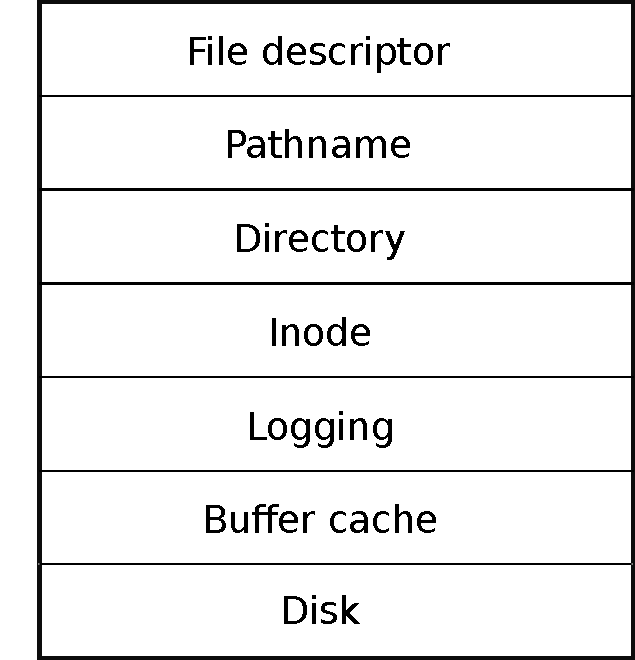
\includegraphics[scale=0.5]{fig/fslayer.pdf}
\caption{xv6 文件系统的层。  }
\label{fig:fslayer}
\end{figure}     

磁盘硬件传统上将磁盘上的数据呈现为 512 字节块的编号序列
    \index{block}   (也称为扇区):
    \index{sector}    扇区 0 是前 512 个字节,扇区 1 是下一个字节,依此类推。操作系统用于其文件系统的块大小可能与磁盘使用的扇区大小不同,但通常块大小是扇区大小的倍数。 Xv6 保存已读入内存的块的副本(类型为对象)
    \lstinline{struct buf}   
    \lineref{kernel/buf.h:/^struct.buf/}    。此结构中存储的数据有时与磁盘不同步:它可能尚未从磁盘读入(磁盘正在处理它,但尚未返回扇区的内容),或者它可能已被软件更新但尚未写入磁盘。  

文件系统必须计划在磁盘上存储 inode 和内容块的位置。为此,xv6 将磁盘分为几个部分,如图~\ref{fig:fslayout}    所示。文件系统不使用块 0(它保存引导扇区)。块 1 称为
    \indextext{superblock}   ;它包含有关文件系统的元数据(文件系统大小(以块为单位)、数据块数量、索引节点数量以及日志中的块数量)。从 2 开始的块保存日志。日志之后是索引节点,每个块有多个索引节点。之后是位图块,跟踪哪些数据块正在使用。其余块为数据块;每个都在位图块中标记为空闲,或者保存文件或目录的内容。超级块由一个单独的程序填充,称为
    \indexcode{mkfs}    ,构建初始文件系统。  

本章的其余部分将讨论每一层,从缓冲区高速缓存开始。留意较低层精心选择的抽象有助于较高层设计的情况。
    \section{缓冲区高速缓存层  }   
    \label{s:bcache}     

缓冲区高速缓存有两个工作:(1)同步对磁盘块的访问,以确保内存中只有一个块的副本,并且一次只有一个内核线程使用该副本; (2) 缓存流行的块,这样就不需要从慢速磁盘重新读取它们。代码在
    \lstinline{bio.c}    。  

buffer cache导出的主要接口包括
    \indexcode{bread}    和
    \indexcode{bwrite}    ;前者获得
    \indextext{buf}    包含可以在内存中读取或修改的块的副本,后者将修改后的缓冲区写入磁盘上的相应块。内核线程必须通过调用释放缓冲区
    \indexcode{brelse}    完成后。缓冲区高速缓存使用每缓冲区睡眠锁来确保一次只有一个线程使用每个缓冲区(以及每个磁盘块);
    \lstinline{bread}    返回一个锁定的缓冲区,并且
    \lstinline{brelse}    释放锁。  

让我们回到缓冲区高速缓存。缓冲区高速缓存具有固定数量的缓冲区来保存磁盘块,这意味着如果文件系统请求高速缓存中尚未存在的块,则缓冲区高速缓存必须回收当前保存其他块的缓冲区。缓冲区高速缓存为新块回收最近最少使用的缓冲区。假设最近最少使用的缓冲区是最不可能很快再次使用的缓冲区。  

   \begin{figure}[t]
\center
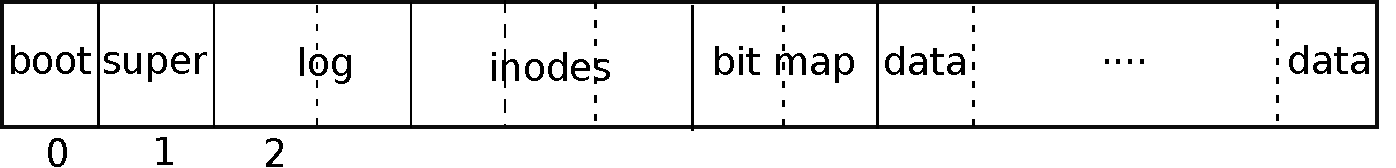
\includegraphics[scale=0.5]{fig/fslayout.pdf}
\caption{xv6 文件系统的结构。  }
\label{fig:fslayout}
\end{figure}   
    \section{代码:缓冲区缓存  }     

缓冲区高速缓存是缓冲区的双向链表。
    \indexcode{main}   
    \lineref{kernel/main.c:/binit/}调用函数\indexcode{binit}    ,使用静态数组     \lstinline{buf} \linerefs{kernel/bio.c:/Create.linked.list/,/^..}/} 中的 NBUF 缓冲区初始化列表。对缓冲区高速缓存的所有其他访问都通过 bcache.head 引用链表,而不是 buf 数组。  

缓冲区有两个与其关联的状态字段。字段
    \indexcode{valid}    指示缓冲区包含该块的副本。字段    \indexcode{disk}    指示缓冲区内容已传递到磁盘,这可能会更改缓冲区(例如,将数据从磁盘写入    \lstinline{data}    )。  

   \lstinline{bread}   
    \lineref{kernel/bio.c:/^bread/}    调用
    \indexcode{bget}    获取给定扇区的缓冲区
    \lineref{kernel/bio.c:/b.=.bget/}    。如果需要从磁盘读取缓冲区,
    \lstinline{bread}    调用
    \indexcode{virtio_disk_rw}    在返回缓冲区之前执行此操作。  

   \lstinline{bget}   
    \lineref{kernel/bio.c:/^bget/}    扫描缓冲区列表以查找具有给定设备号和扇区号的缓冲区
\linerefs{kernel/bio.c:/Is.the.block.already/,/^..}    /}。如果有这样的缓冲区的话
    \indexcode{bget}    获取缓冲区的睡眠锁。
 然后    \lstinline{bget}    返回锁定的缓冲区。  

如果给定扇区没有缓存缓冲区,
    \indexcode{bget}    必须创建一个,可能会重用保存不同扇区的缓冲区。它第二次扫描缓冲区列表,查找未使用的缓冲区 (    \lstinline{b->refcnt = 0}    );可以使用任何此类缓冲区。
    \lstinline{bget}    编辑缓冲区元数据以记录新的设备和扇区号并获取其睡眠锁。请注意,分配
    \lstinline{b->valid = 0}    确保
    \lstinline{bread}    将从磁盘读取块数据,而不是错误地使用缓冲区以前的内容。  

重要的是,每个磁盘扇区最多有一个缓存缓冲区,以确保读取器看到写入,并且因为文件系统使用缓冲区上的锁来进行同步。
    \lstinline{bget}    通过保持
    \lstinline{bache.lock}    从第一个循环检查该块是否已缓存到第二个循环声明该块现在已被缓存(通过设置
    \lstinline{dev}    ,
    \lstinline{blockno}    和
    \lstinline{refcnt}   )。这会导致对块是否存在的检查以及(如果不存在)对保存该块的缓冲区的指定是原子的。  

这是安全的
    \lstinline{bget}    获取缓冲区外部的睡眠锁
    \lstinline{bcache.lock}    临界区,由于非零
    \lstinline{b->refcnt}    防止缓冲区被重新用于不同的磁盘块。睡眠锁保护块缓冲内容的读写,而
    \lstinline{bcache.lock}    保护有关缓存哪些块的信息。  

如果所有缓冲区都忙,则说明有太多进程同时执行文件系统调用;
    \lstinline{bget}    出现Panic。更优雅的响应可能是休眠直到缓冲区空闲,尽管这样可能会出现死锁。  

一次
    \indexcode{bread}    已读取磁盘(如果需要)并将缓冲区返回给其调用者,调用者独占使用该缓冲区并可以读取或写入数据字节。如果调用者确实修改了缓冲区,则必须调用
    \indexcode{bwrite}    在释放缓冲区之前将更改的数据写入磁盘。
    \lstinline{bwrite}   
    \lineref{kernel/bio.c:/^bwrite/}    调用
    \indexcode{virtio_disk_rw}    与磁盘硬件对话。  

当调用者使用完缓冲区后,它必须调用
    \indexcode{brelse}    来释放它。 (名字
    \lstinline{brelse}    是 b-release 的缩写,虽然神秘但值得学习:它起源于 Unix,也用于 BSD、Linux 和 Solaris。)
    \lstinline{brelse}   
    \lineref{kernel/bio.c:/^brelse/}    释放睡眠锁并将缓冲区移动到链表的前面
    \linerefs{kernel/bio.c:/b->next->prev.=.b->prev/,/bcache.head.next.=.b/}    。移动缓冲区会导致列表按照缓冲区最近使用的时间(意味着释放)进行排序:列表中的第一个缓冲区是最近使用的,最后一个缓冲区是最近最少使用的。中的两个循环
    \lstinline{bget}    利用了这一点:在最坏的情况下,对现有缓冲区的扫描必须处理整个列表,但首先检查最近使用的缓冲区(从
    \lstinline{bcache.head}    及以下
 当存在良好的引用局部性时,   \lstinline{next}    指针)将减少扫描时间。选择要重用的缓冲区的扫描通过向后扫描来选择最近最少使用的缓冲区(以下
    \lstinline{prev}    指针)。
    \section{日志层  }     

文件系统设计中最有趣的问题之一是崩溃恢复。出现此问题的原因是许多文件系统操作涉及对磁盘的多次写入,并且写入子集后发生崩溃可能会使磁盘上的文件系统处于不一致的状态。例如,假设在文件截断期间发生崩溃(将文件的长度设置为零并释放其内容块)。根据磁盘写入的顺序,崩溃可能会留下一个带有对标记为空闲的内容块的引用的索引节点,也可能会留下一个已分配但未引用的内容块。  

后者相对良性,但引用已释放块的索引节点在重新启动后可能会导致严重问题。重新启动后,内核可能会将该块分配给另一个文件,现在我们有两个不同的文件无意中指向同一个块。如果 xv6 支持多个用户,这种情况可能会成为安全问题,因为旧文件的所有者将能够读取和写入由不同用户拥有的新文件中的块。  

Xv6 通过简单的日志记录形式解决了文件系统操作期间的崩溃问题。 xv6 系统调用不直接写入磁盘文件系统数据结构。相反,它将它希望进行的所有磁盘写入的描述放在一个
 磁盘上的    \indextext{log}   。一旦系统调用记录了所有写入,它就会写入一个特殊的
    \indextext{commit}    记录到磁盘,表明日志包含完整的操作。此时,系统调用会将写入内容复制到磁盘文件系统数据结构。这些写入完成后,系统调用会擦除磁盘上的日志。  

如果系统崩溃并重新启动,文件系统代码会在运行任何进程之前按如下方式从崩溃中恢复。如果日志被标记为包含完整操作,则恢复代码会将写入内容复制到磁盘文件系统中它们所属的位置。如果日志未标记为包含完整操作,则恢复代码将忽略该日志。恢复代码通过擦除日志来完成。  

为什么xv6的日志解决了文件系统操作崩溃的问题?如果崩溃发生在操作提交之前,则磁盘上的日志将不会被标记为完成,恢复代码将忽略它,并且磁盘的状态将就像操作尚未开始一样。如果崩溃发生在操作提交之后,那么恢复将重放该操作的所有写入,如果该操作已开始将它们写入磁盘数据结构,则可能会重复它们。在任何一种情况下,日志都会使操作相对于崩溃而言是原子的:恢复后,操作的所有写入要么都出现在磁盘上,要么都不出现。
    \section{日志设计  }     

日志驻留在超级块中指定的已知固定位置。它由一个标头块组成,后跟一系列更新的块副本(“记录块”)。标头块包含一组扇区号,每个扇区号对应每个已记录的块,以及日志块的计数。磁盘上标头块中的计数要么为零,表示日志中没有事务,要么非零,表示日志包含具有指定数量的已记录块的完整已提交事务。 Xv6 在事务提交时(而不是之前)写入标头块,并在将记录的块复制到文件系统后将计数设置为零。因此,事务中途崩溃将导致日志标头块中的计数为零;提交后的崩溃将导致非零计数。  

每个系统调用的代码指示写入序列的开始和结束,这些写入序列对于崩溃而言必须是原子的。为了允许不同进程并发执行文件系统操作,日志系统可以将多个系统调用的写入累积到一个事务中。因此,单个提交可能涉及多个完整系统调用的写入。为了避免跨事务分割系统调用,日志系统仅在没有文件系统系统调用正在进行时提交。  

一起提交多个事务的想法被称为
    \indextext{group commit}    。组提交减少了磁盘操作的数量,因为它将一次提交的固定成本分摊到多个操作上。组提交还可以同时为磁盘系统提供更多并发写入,也许允许磁盘在单个磁盘旋转期间将它们全部写入。 xv6的virtio驱动不支持这种
    \indextext{batching}    ,但 xv6 的文件系统设计允许这样做。  

Xv6 在磁盘上指定固定数量的空间来保存日志。事务中系统调用写入的块总数必须适合该空间。这有两个后果。不允许单个系统调用写入多于日志空间的不同块。对于大多数系统调用来说这不是问题,但是其中两个系统调用可能会写入许多块:
    \indexcode{write}    和
    \indexcode{unlink}    。大文件写入可能会写入很多数据块和很多位图块以及一个inode块;取消链接大文件可能会写入许多位图块和一个索引节点。 Xv6 的写入系统调用将大型写入分解为多个适合日志的较小写入,并且
    \lstinline{unlink}    不会引起问题,因为实际上 xv6 文件系统仅使用一个位图块。有限日志空间的另一个后果是日志系统不允许系统调用启动,除非确定系统调用的写入适合日志中的剩余空间。
    \section{代码:记录  }     

系统调用中日志的典型用法如下:
\begin{lstlisting}[]
begin_op();
...
bp = bread(...);
bp->data[...] = ...;
log_write(bp);
...
end_op();
\end{lstlisting}     

   \indexcode{begin_op}   
    \lineref{kernel/log.c:/^begin.op/}    一直等待,直到日志系统当前未提交,并且有足够的未保留日志空间来保存此调用的写入。
    \lstinline{log.outstanding}    统计保留日志空间的系统调用数量;总保留空间为
    \lstinline{log.outstanding}    次
    \lstinline{MAXOPBLOCKS}    。递增
    \lstinline{log.outstanding}    既保留空间又防止在此系统调用期间发生提交。该代码保守地假设每个系统调用可能会写入
    \lstinline{MAXOPBLOCKS}    个不同的块。  

   \indexcode{log_write}   
    \lineref{kernel/log.c:/^log.write/}    充当代理
    \indexcode{bwrite}    。它在内存中记录块的扇区号,在磁盘上的日志中为其保留一个槽位,并将缓冲区固定在块缓存中以防止块缓存将其驱逐。该块必须保留在缓存中直到提交:在此之前,缓存的副本是修改的唯一记录;直到提交之后才能将其写入磁盘上的位置;并且同一事务中的其他读取必须看到修改。
    \lstinline{log_write}    会注意到在单个事务期间某个块被多次写入的情况,并在日志中为该块分配相同的槽。这种优化通常称为
    \indextext{absorption}    。例如,常见的是,包含多个文件的索引节点的磁盘块在一个事务内被写入多次。通过将多个磁盘写入吸收为一个,文件系统可以节省日志空间并可以获得更好的性能,因为只需将磁盘块的一份副本写入磁盘。  

   \indexcode{end_op}   
    \lineref{kernel/log.c:/^end.op/}    首先减少未完成的系统调用的计数。如果计数现在为零,则它通过调用提交当前事务
    \lstinline{commit().}    此过程有四个阶段。
    \lstinline{write_log()}   
    \lineref{kernel/log.c:/^write.log/}    将事务中修改的每个块从缓冲区高速缓存复制到磁盘上日志中的槽。
    \lstinline{write_head()}   
    \lineref{kernel/log.c:/^write.head/}    将标头块写入磁盘:这是提交点,写入后的崩溃将导致恢复重放日志中事务的写入。
    \indexcode{install_trans}   
    \lineref{kernel/log.c:/^install_trans/}    从日志中读取每个块并将其写入文件系统中的适当位置。最后
    \lstinline{end_op}    写入计数为零的日志标头;这必须在下一个事务开始写入记录块之前发生,这样崩溃就不会导致使用一个事务的标头和后续事务的记录块进行恢复。  

   \indexcode{recover_from_log}   
    \lineref{kernel/log.c:/^recover_from_log/}    是从
    \indexcode{initlog}   
    \lineref{kernel/log.c:/^initlog/}    ,在第一个用户进程运行之前启动期间从    \indexcode{fsinit}       \lineref{kernel/fs.c:/^fsinit/}    调用
    \lineref{kernel/proc.c:/fsinit/}    。它读取日志头,并模仿
    \lstinline{end_op}    如果标头指示日志包含已提交的事务。  

日志的使用示例发生在
    \indexcode{filewrite}   
    \lineref{kernel/file.c:/^filewrite/}    。交易看起来像这样:
\begin{lstlisting}[]
begin_op();
ilock(f->ip);
r = writei(f->ip, ...);
iunlock(f->ip);
end_op();
\end{lstlisting}    此代码包含在一个循环中,该循环将大型写入一次分解为几个扇区的单独事务,以避免日志溢出。致电给
    \indexcode{writei}    写入许多块作为此事务的一部分:文件的索引节点、一个或多个位图块以及一些数据块。
    \section{代码:块分配器  }     

文件和目录内容存储在磁盘块中,必须从空闲池中分配磁盘块。 Xv6 的块分配器在磁盘上维护一个空闲位图,每个块一位。零位表示对应的块是空闲的;一位表示该块正在使用中。该程序
    \lstinline{mkfs}    设置与引导扇区、超级块、日志块、索引节点块和位图块相对应的位。  

块分配器提供两个功能:
    \indexcode{balloc}    分配一个新的磁盘块,并且
    \indexcode{bfree}    释放一个块。
    \lstinline{balloc}    中的循环
    \lstinline{balloc}    在
    \lineref{kernel/fs.c:/^..for.b.=.0/}    考虑每个块,从块 0 开始直到
    \lstinline{sb.size}    ,文件系统中的块数。它查找位图位为零的块,表明它是空闲的。如果
    \lstinline{balloc}    找到这样的块,它更新位图并返回该块。为了提高效率,循环被分成两部分。外循环读取每个位图位块。内部循环检查单个位图块中的所有位每块 (    \lstinline{BPB}    ) 位。由于缓冲区高速缓存一次只允许一个进程使用任意一个位图块,因此可以防止两个进程同时尝试分配一个块时可能发生的竞争。  

   \lstinline{bfree}   
    \lineref{kernel/fs.c:/^bfree/}    找到正确的位图块并清除正确的位。再次暗示独家使用
    \lstinline{bread}    和
    \lstinline{brelse}    避免了显式锁定的需要。  

与本章其余部分描述的大部分代码一样,
    \lstinline{balloc}    和
    \lstinline{bfree}    必须在事务内部调用。
    \section{索引节点层  }     

术语
    \indextext{inode}    可以具有两个相关含义之一。它可能指的是包含文件大小和数据块编号列表的磁盘数据结构。或者“inode”可能指的是内存中的inode,其中包含磁盘上的inode 的副本以及内核中所需的额外信息。  

磁盘上的索引节点被打包到称为索引节点块的磁盘连续区域中。每个 inode 的大小相同,因此给定数字 n,很容易找到磁盘上的第 n 个 inode。事实上,这个数字n,称为inode编号或i-number,是在实现中识别inode的方式。  

磁盘上的 inode 定义为
    \indexcode{struct dinode}   
    \lineref{kernel/fs.h:/^struct.dinode/}    。这
    \lstinline{type}    字段区分文件、目录和特殊文件(设备)。零类型表示磁盘上的索引节点是空闲的。这
    \lstinline{nlink}    字段对引用此 inode 的目录条目数进行计数,以便识别何时应释放磁盘 inode 及其数据块。这
    \lstinline{size}   字段记录文件内容的字节数。这
    \lstinline{addrs}    数组记录保存文件内容的磁盘块的块号。  

内核将一组活动 inode 保存在内存中名为    \indexcode{itable}    的表中;
    \indexcode{struct inode}   
    \lineref{kernel/file.h:/^struct.inode/}    是 a 的内存中副本
    \lstinline{struct}   
 磁盘上的    \lstinline{dinode}   。仅当存在引用该 inode 的 C 指针时,内核才会在内存中存储该 inode。这
    \lstinline{ref}    字段计算引用内存中 inode 的 C 指针的数量,如果引用计数降至零,则内核会从内存中丢弃该 inode。这
    \indexcode{iget}    和
    \indexcode{iput}    函数获取和释放指向 inode 的指针,修改引用计数。指向 inode 的指针可以来自文件描述符、当前工作目录和瞬态内核代码,例如
    \lstinline{exec}    。  

xv6的sinode代码中有四种锁或类似锁的机制。
    \lstinline{itable.lock}    保护索引节点在索引节点表中最多出现一次的不变量,以及内存中索引节点的不变量
    \lstinline{ref}    字段计算内存中指向 inode 的指针的数量。每个内存中的 inode 都有一个
    \lstinline{lock}    字段包含睡眠锁,它确保对 inode 的字段(例如文件长度)以及 inode 的文件或目录内容块的独占访问。一个索引节点
    \lstinline{ref}   ,如果它大于零,则导致系统维护表中的索引节点,并且不会为不同的索引节点重新使用表条目。最后,每个 inode 包含一个
    \lstinline{nlink}    字段(在磁盘上,如果在内存中则复制到内存中),用于计算引用文件的目录条目的数量;如果其链接计数大于零,xv6 将不会释放索引节点。  

A
    \lstinline{struct}   
    \lstinline{inode}    返回的指针
    \lstinline{iget()}    保证有效,直到相应的调用
    \lstinline{iput()}    ;索引节点不会被删除,并且指针引用的内存不会被重新用于不同的索引节点。
    \lstinline{iget()}    提供对 inode 的非独占访问,因此可以有多个指向同一 inode 的指针。文件系统代码的许多部分都依赖于这种行为
    \lstinline{iget()}    ,既可以保存对 inode 的长期引用(例如打开的文件和当前目录),又可以防止竞争,同时避免操作多个 inode 的代码(例如路径名查找)中出现死锁。  

这
    \lstinline{struct}   
    \lstinline{inode}    那个
    \lstinline{iget}    返回的内容可能没有任何有用的内容。为了确保它拥有磁盘节点上的副本,代码必须调用
    \indexcode{ilock}    。这会锁定索引节点(这样其他进程就不能
    \lstinline{ilock}    它)并从磁盘读取 inode(如果尚未读取)。
    \lstinline{iunlock}    释放 inode 上的锁。将 inode 指针的获取与锁定分开有助于避免某些情况下的死锁,例如在目录查找期间。多个进程可以保存一个指向 inode 返回的 C 指针
    \lstinline{iget}    ,但一次只有一个进程可以锁定 inode。  

inode 表仅存储内核代码或数据结构保存 C 指针的 inode。它的主要工作是同步多个进程的访问。 inode表也恰好缓存了常用的inode,但缓存是次要的;如果频繁使用某个索引节点,缓冲区高速缓存可能会将其保留在内存中。修改内存中 inode 的代码将其写入磁盘
    \lstinline{iupdate}    。
    \section{代码:索引节点  }     

要分配新的 inode(例如,创建文件时),xv6 调用
    \indexcode{ialloc}   
    \lineref{kernel/fs.c:/^ialloc/}    。
    \lstinline{ialloc}    类似于
    \indexcode{balloc}   :它循环遍历磁盘上的 inode 结构,一次一个块,寻找标记为空闲的一个。当它找到一个时,它会通过写新的来声明它
    \lstinline{type}    到磁盘,然后从 inode 表返回一个条目,并通过尾部调用
    \indexcode{iget}   
\lineref{kernel/fs.c:/return.iget        \(dev..inum\)        /}   。正确的操作是
    \lstinline{ialloc}    取决于这样一个事实:一次只有一个进程可以持有对
    \lstinline{bp}   :
    \lstinline{ialloc}    可以确定其他进程不会同时看到该 inode 可用并尝试声明它。  

   \lstinline{iget}   
    \lineref{kernel/fs.c:/^iget/}    在索引节点表中查找活动条目 (    \lstinline{ip->ref}   
    \lstinline{>}   
    \lstinline{0}    )以及所需的设备和 inode 号。如果找到,它将返回对该 inode 的新引用
\linerefs{kernel/fs.c:/^....if.ip->ref.>.0/,/^....}    /}。作为
    \indexcode{iget}   扫描,记录第一个空槽的位置
    \linerefs{kernel/fs.c:/^....if.empty.==.0/,/empty.=.ip/}    ,如果需要分配表条目,则使用它。  

代码必须在读取或写入其元数据或内容之前 使用\indexcode{ilock}锁定 inode。
    \lstinline{ilock}   
    \lineref{kernel/fs.c:/^ilock/}    为此使用睡眠锁。一次
    \indexcode{ilock}    具有对 inode 的独占访问权限,如果需要,它会从磁盘(更可能是缓冲区高速缓存)读取 inode。功能
    \indexcode{iunlock}   
    \lineref{kernel/fs.c:/^iunlock/}    释放睡眠锁,这可能会导致任何正在睡眠的进程被唤醒。  

   \lstinline{iput}   
    \lineref{kernel/fs.c:/^iput/}    通过减少引用计数来释放指向 inode 的 C 指针
    \lineref{kernel/fs.c:/^..ip->ref--/}    。如果这是最后一次引用,则 inode 表中的 inode 插槽现在是空闲的,并且可以重新用于不同的 inode。  

如果
    \indexcode{iput}    发现没有对 inode 的 C 指针引用,并且 inode 没有到它的链接(出现在 nodirectory 中),则必须释放 inode 及其数据块。
    \lstinline{iput}    调用
    \indexcode{itrunc}    将文件截断至零字节,释放数据块;将 inode 类型设置为 0(未分配);并将 inode 写入磁盘
    \lineref{kernel/fs.c:/inode.has.no.links.and/}    。  

锁定协议在
    \indexcode{iput}    释放 inode 的情况值得仔细研究。一个危险是并发线程可能正在等待
    \lstinline{ilock}    使用此 inode(例如,读取文件或列出目录),并且不会准备好发现该 inode 不再分配。这种情况不会发生,因为如果没有指向内存中 inode 的链接,系统调用就无法获取指向该 inode 的指针,并且
    \lstinline{ip->ref}    就是其中之一。该引用是调用线程所拥有的引用
    \lstinline{iput}    。确实如此
    \lstinline{iput}    检查引用计数是否超出其值之一
    \lstinline{itable.lock}    关键部分,但此时已知链接计数为零,因此没有线程会尝试获取新引用。另一个主要危险是并发调用
    \lstinline{ialloc}    可能会选择与
    \lstinline{iput}    正在释放。这只能发生在
    \lstinline{iupdate}    写入磁盘,以便 inode 的类型为零。这个种族是良性的;分配线程将在读取或写入 inode 之前礼貌地等待获取 inode 的睡眠锁,此时
    \lstinline{iput}    就完成了。  

   \lstinline{iput()}    可以写入磁盘。这意味着使用该文件系统的任何系统调用都可以写入磁盘,因为该系统调用可能是最后一个引用该文件的系统调用。甚至像这样打电话
    \lstinline{read()}    似乎是只读的,最终可能会调用
    \lstinline{iput().}    反过来,这意味着即使是只读系统调用,如果它们使用文件系统,也必须包装在事务中。  

之间存在着具有挑战性的互动
    \lstinline{iput()}    并崩溃。
 当文件的链接计数降至零时,   \lstinline{iput()}    不会立即截断文件,因为某些进程可能仍保留对内存中 inode 的引用:进程可能仍在读取和写入文件,因为它已成功打开文件。但是,如果崩溃发生在最接近该文件的文件描述符的最后一个进程之前,则该文件将被标记为已在磁盘上分配,但没有目录条目指向它。  

文件系统以两种方式之一处理这种情况。简单的解决方案是,在恢复时,重新启动后,文件系统会扫描整个文件系统以查找标记为已分配但没有指向它们的目录条目的文件。如果存在任何此类文件,则它可以释放这些文件。  

第二种解决方案不需要扫描文件系统。在此解决方案中,文件系统将链接计数降至零但引用计数不为零的文件的索引节点号记录在磁盘上(例如,在超级块中)。如果文件系统在其引用计数达到 0 时删除该文件,则会通过从列表中删除该 inode 来更新磁盘列表。恢复时,文件系统释放列表中的所有文件。  

Xv6 没有实现这两种解决方案,这意味着索引节点可能会被标记为在磁盘上分配,即使它们不再使用。这意味着随着时间的推移,xv6 会面临磁盘空间不足的风险。
    \section{代码:inode内容  }     

   \begin{figure}[t]
\center
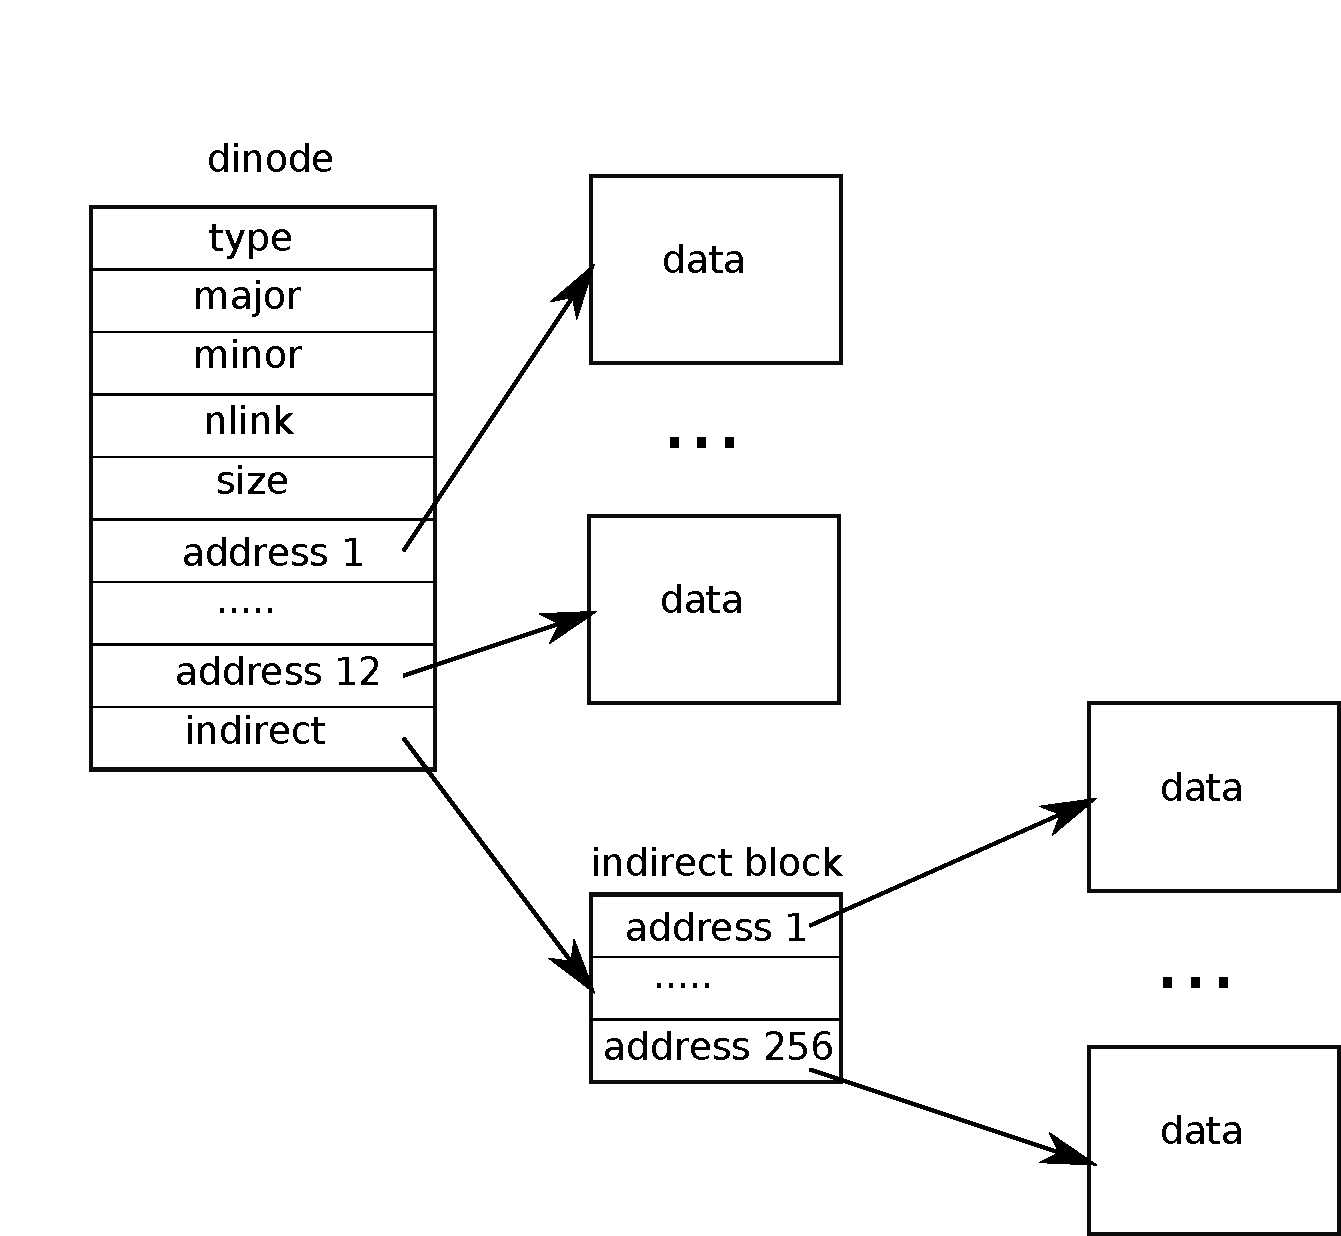
\includegraphics[scale=0.5]{fig/inode.pdf}
\caption{磁盘上文件的表示。  }
\label{fig:inode}
\end{figure}     

磁盘上的 inode 结构,
    \indexcode{struct dinode}    ,包含大小和块编号数组(参见图~    \ref{fig:inode}    )。 inode 数据可在列出的块中找到
    \lstinline{dinode}    的
    \lstinline{addrs}    数组。首先
 第一个列出了    \indexcode{NDIRECT}    数据块
 数组中的    \lstinline{NDIRECT}    条目;这些块被称为
    \indextext{direct blocks}    。下一个
    \indexcode{NINDIRECT}    数据块不在索引节点中列出,而是在称为
    \indextext{indirect block}    。最后一个条目在
    \lstinline{addrs}    数组给出间接块的地址。因此前 12 kB (
    \lstinline{NDIRECT}   
    \lstinline{x}   
    \indexcode{BSIZE}    )文件的字节可以从 inode 中列出的块加载,而下一个
    \lstinline{256}    kB (
    \lstinline{NINDIRECT}   
    \lstinline{x}   
    \lstinline{BSIZE}    )字节只能在查阅间接块后加载。这是一种很好的磁盘表示形式,但对于客户端来说却很复杂。功能
    \indexcode{bmap}    管理表示,以便更高级别的例程,例如
    \indexcode{readi}    和
 我们很快就会看到    \indexcode{writei}    不需要管理这种复杂性。
    \lstinline{bmap}    返回磁盘块号
    \lstinline{bn}    '索引节点的数据块
    \lstinline{ip}    。如果
    \lstinline{ip}   还没有这样的块,
    \lstinline{bmap}    分配 1。  

功能
    \indexcode{bmap}   
    \lineref{kernel/fs.c:/^bmap/}    首先选择简单的情况:第一个
    \indexcode{NDIRECT}    块在 inode 本身中列出
    \linerefs{kernel/fs.c:/^..if.bn.<.NDIRECT/,/^..}/}。下一个
    \indexcode{NINDIRECT}    块列在间接块中
    \lstinline{ip->addrs[NDIRECT]}    。
    \lstinline{bmap}    读取间接块
    \lineref{kernel/fs.c:/bp.=.bread.ip->dev..addr/}    然后从块内的正确位置读取块号
    \lineref{kernel/fs.c:/a.=..uint\*.bp->data/}    。如果区块数量超过
    \lstinline{NDIRECT+NINDIRECT}    ,
    \lstinline{bmap}    Panic;
    \lstinline{writei}    包含防止这种情况发生的检查
    \lineref{kernel/fs.c:/off...n...MAXFILE.BSIZE/}    。  

   \lstinline{bmap}    根据需要分配块。一个
    \lstinline{ip->addrs[]}    或间接条目为零表示未分配任何块。作为
    \lstinline{bmap}    遇到零,它用新鲜块的数量替换它们,按需分配
    \linerefs{kernel/fs.c:/^....if..addr.=.*==.0/,/./}   
    \linerefs{kernel/fs.c:/^....if..addr.*NDIRECT.*==.0/,/./}    。  

   \indexcode{itrunc}    释放文件的块,将索引节点的大小重置为零。
    \lstinline{itrunc}   
    \lineref{kernel/fs.c:/^itrunc/}    首先释放直接块
    \linerefs{kernel/fs.c:/^..for.i.=.0.*NDIRECT/,/^..}    /},然后是间接块中列出的
    \linerefs{kernel/fs.c:/^....for.j.=.0.*NINDIRECT/,/^....}    /},最后是间接块本身
    \linerefs{kernel/fs.c:/^....bfree.*NDIRECT/,/./}    。  

   \lstinline{bmap}    使之变得容易
    \indexcode{readi}    和
    \indexcode{writei}    获取 inode 的数据。
    \lstinline{readi}   
    \lineref{kernel/fs.c:/^readi/}    首先确保偏移量和计数不超出文件末尾。从文件末尾开始读取会返回错误
    \linerefs{kernel/fs.c:/^..if.off.>.ip->size/,/./}    从文件末尾开始或越过文件末尾的读取返回的字节数少于请求的字节数
    \linerefs{kernel/fs.c:/^..if.off.\+.n.>.ip->size/,/./}    。主循环处理文件的每个块,将数据从缓冲区复制到
    \lstinline{dst}   
\linerefs{kernel/fs.c:/^..for.tot=0/,/^..}    /}。
    \indexcode{writei}   
    \lineref{kernel/fs.c:/^writei/}    等同于
    \indexcode{readi}    ,有三个例外:从文件末尾开始或越过文件末尾的写入增大文件,直至最大文件大小
    \linerefs{kernel/fs.c:/^..if.off.\+.n.>.MAXFILE/,/./}    ;循环将数据复制到缓冲区而不是输出
    \lineref{kernel/fs.c:/memmove.*bp->data/}    ;如果写入扩展了文件,
    \indexcode{writei}    必须更新其大小
\linerefs{kernel/fs.c:/^..if.n.>.0./,/^..}    /}。  

功能
    \indexcode{stati}   
\lineref{kernel/fs.c:/^stati        \(/}将 inode 元数据复制到
\lstinline{stat} 结构,通过以下方式向用户程序公开
\indexcode{stat}系统调用。
\section{代码:目录层   }     

目录的内部实现与文件非常相似。它的索引节点有类型
    \indexcode{T_DIR}    及其数据是目录条目的序列。每个条目都是一个
    \indexcode{struct dirent}   
    \lineref{kernel/fs.h:/^struct.dirent/}     { 
56   } ,包含名称和索引节点号。名字最多是
    \indexcode{DIRSIZ}    (14) 个字符;如果较短,则以 NULL (0) 字节终止。 inode 号为零的目录条目是免费的。  

函数
    \indexcode{dirlookup}   
    \lineref{kernel/fs.c}     { 
552   }  在目录中搜索具有给定名称的条目。如果找到一个,它返回一个指向相应 inode 的指针,解锁并设置
    \lstinline{*poff}    到目录中条目的字节偏移量,以防调用者希望编辑它。如果
    \lstinline{dirlookup}    找到具有正确名称的条目,它会更新
    \lstinline{*poff}    并返回通过以下方式获得的解锁 inode
    \indexcode{iget}    。
    \lstinline{dirlookup}    的原因是
    \lstinline{iget}    返回未锁定的索引节点。来电者已锁定
    \lstinline{dp}    ,所以如果查找的是
    \indexcode{.}    ,当前目录的别名,尝试在返回之前锁定inode会尝试重新锁定
    \lstinline{dp}    和死锁。 (还有更复杂的死锁场景,涉及多个进程和
    \indexcode{..}    ,父目录的别名;
    \lstinline{.}    不是唯一的问题。)调用者可以解锁
    \lstinline{dp}    然后锁定
    \lstinline{ip}    ,确保它一次只持有一把锁。  

功能
    \indexcode{dirlink}   
    \lineref{kernel/fs.c:/^dirlink/}  将具有给定名称和 inode 编号的新目录条目写入目录
    \lstinline{dp}    。如果该名称已经存在,
    \lstinline{dirlink}    返回错误
    \linerefs{kernel/fs.c:/Check.that.name.is.not.present/,/^..}/} 。主循环读取目录条目以查找未分配的条目。当它找到一个时,它会提前停止循环
    \linerefs{kernel/fs.c:/^....if.de.inum.==.0/,/./} ,与
    \lstinline{off}    设置为可用条目的偏移量。否则,循环结束于
    \lstinline{off}    设置为
    \lstinline{dp->size}    。无论哪种方式,
 然后,   \lstinline{dirlink}    通过在偏移处写入来向目录添加一个新条目
    \lstinline{off}   
    \section{代码:路径名   }     

路径名查找涉及一系列调用
    \indexcode{dirlookup}    ,每个路径组件一个。
    \lstinline{namei}   
    \linerefs{kernel/fs.c:/^..strncpy/,/panic/}  评估
    \lstinline{path}   并返回相应的
    \lstinline{inode}    。功能
    \indexcode{nameiparent}    是一个变体:它在最后一个元素之前停止,返回父目录的 inode 并将最终元素复制到
    \lstinline{name}    。两者都调用广义函数
    \indexcode{namex}    来做真正的工作。  

   \lstinline{namex}   
   \lineref{kernel/fs.c:/^namex/}  首先决定路径评估从哪里开始。如果路径以斜杠开头,则从根开始求值;否则,从当前目录开始      \indexcode{skipelem}    依次考虑路径的每个元素
   \linerefs{kernel/fs.c:/..if.\*path.==....\)        /,/idup/}     。循环的每次迭代都必须查找
 当前 inode 中的    \lstinline{name}   
    \lstinline{ip}    。迭代从锁定开始
    \lstinline{ip}    并检查它是否是一个目录。如果没有,则查找失败
    \linerefs{kernel/fs.c:/^....ilock.ip/,/^....}    /}。 (锁定
    \lstinline{ip}    是必要的,不是因为
    \lstinline{ip->type}    可以在脚下改变——它不能——但是因为直到
    \indexcode{ilock}    运行,
 不保证    \lstinline{ip->type}    已从磁盘加载。)如果调用是
    \indexcode{nameiparent}    这是最后一个路径元素,循环提前停止,根据定义
    \lstinline{nameiparent}    ;最终路径元素已被复制到
    \lstinline{name}   ,所以
    \indexcode{namex}   只需返回解锁的
    \lstinline{ip}   
    \linerefs{kernel/fs.c:/^....if.nameiparent/,/^....}    /}。最后,循环使用以下命令查找路径元素
    \indexcode{dirlookup}    并通过设置为下一次迭代做准备
    \lstinline{ip = next}   
    \linerefs{kernel/fs.c:/^....if..next.*dirlookup/,/^....ip.=.next/}    。当循环耗尽路径元素时,返回
    \lstinline{ip}    。  

步骤
    \lstinline{namex}    可能需要很长时间才能完成:它可能涉及多个磁盘操作来读取路径名中遍历的目录的 inode 和目录块(如果它们不在缓冲区高速缓存中)。 Xv6 经过精心设计,因此如果调用
    \lstinline{namex}    被一个内核线程阻塞在磁盘 I/O 上,查找不同路径名的另一个内核线程可以同时进行。
    \lstinline{namex}    分别锁定路径中的每个目录,以便不同目录中的查找可以并行进行。  

这种并发带来了一些挑战。例如,当一个内核线程正在查找路径名时,另一个内核线程可能会通过取消链接目录来更改目录树。潜在的风险是查找可能正在搜索已被另一个内核线程删除的目录,并且其块已被重新用于另一个目录或文件。  

Xv6 避免了这样的竞争。例如,执行时
    \lstinline{dirlookup}    中
    \lstinline{namex}    ,查找线程持有目录的锁并且
    \lstinline{dirlookup}    返回一个使用以下方法获得的 inode
    \lstinline{iget}    。
    \lstinline{iget}    增加 inode 的引用计数。仅在收到来自的索引节点后
    \lstinline{dirlookup}    确实
    \lstinline{namex}    释放目录上的锁。现在另一个线程可能会取消该 inode 与目录的链接,但 xv6 还不会删除该 inode,因为该 inode 的引用计数仍然大于零。  

另一个风险是僵局。例如,
    \lstinline{next}    指向与以下相同的 inode
 查找“.”时的    \lstinline{ip}   。锁定
    \lstinline{next}    释放锁之前
    \lstinline{ip}    会导致死锁。为了避免这种僵局,
    \lstinline{namex}    在获取锁定之前解锁目录
    \lstinline{next}    。在这里我们再次看到为什么两者之间的分离
    \lstinline{iget}    和
    \lstinline{ilock}    很重要。
    \section{文件描述符层  }     

Unix 界面的一个很酷的方面是,Unix 中的大多数资源都以文件的形式表示,包括控制台、管道等设备,当然还有真实的文件。文件描述符层是实现这种一致性的层。  

Xv6 为每个进程提供了自己的打开文件表或文件描述符,正如我们在 Chapter~\ref{CH:UNIX}    中看到的那样。每个打开的文件都由一个表示
    \indexcode{struct file}   
    \lineref{kernel/file.h:/^struct.file/}    ,它是一个 inode 或一个管道的包装器,加上一个 I/O 偏移量。每次致电
    \indexcode{open}    创建一个新的打开文件(一个新的
    \lstinline{struct}   
    \lstinline{file}    ):如果多个进程独立打开同一个文件,不同的实例将有不同的 I/O 偏移量。另一方面,单个打开的文件(相同
    \lstinline{struct}   
    \lstinline{file}    )可以在一个进程的文件表中多次出现,也可以在多个进程的文件表中出现。如果使用一个进程就会发生这种情况
    \lstinline{open}    打开文件,然后使用创建别名
    \indexcode{dup}    或与孩子分享
    \indexcode{fork}    。引用计数跟踪对特定打开文件的引用数量。文件可以打开以进行读取或写入或两者兼而有之。这
    \lstinline{readable}    和
    \lstinline{writable}    字段对此进行跟踪。  

系统中所有打开的文件都保存在一个全局文件表中,
    \indexcode{ftable}    。文件表具有分配文件(    \indexcode{filealloc}    )、创建重复引用(    \indexcode{filedup}    )、释放引用(    \indexcode{fileclose}    )以及读写数据(    \indexcode{fileread}    和
    \indexcode{filewrite}   )。  

前三个遵循现在熟悉的形式。
    \lstinline{filealloc}   
    \lineref{kernel/file.c:/^filealloc/}    扫描文件表以查找未引用的文件 (    \lstinline{f->ref}   
    \lstinline{==}   
    \lstinline{0}    )并返回一个新的引用;
    \indexcode{filedup}   
    \lineref{kernel/file.c:/^filedup/}    增加引用计数;并且
    \indexcode{fileclose}   
    \lineref{kernel/file.c:/^fileclose/}    减少它。当文件的引用计数达到零时,
    \lstinline{fileclose}    根据类型释放底层管道或索引节点。  

功能
    \indexcode{filestat}    ,
    \indexcode{fileread}    和
    \indexcode{filewrite}    实现
    \indexcode{stat}    ,
    \indexcode{read}    和
 对文件的    \indexcode{write}    操作。
    \lstinline{filestat}   
    \lineref{kernel/file.c:/^filestat/}    仅允许在 inode 和调用上
    \indexcode{stati}    。
    \lstinline{fileread}    和
    \lstinline{filewrite}    检查打开模式是否允许该操作,然后将调用传递给管道或 inode 实现。如果文件代表一个 inode,
    \lstinline{fileread}    和
    \lstinline{filewrite}    使用 I/O 偏移量作为操作的偏移量,然后向前推进
    \linerefs{kernel/file.c:/readi/,/./}   
    \linerefs{kernel/file.c:/writei/,/./}    。管道没有偏移的概念。回想一下,inode 函数需要调用者处理锁定
    \linerefs{kernel/file.c:/stati/-1,/iunlock/}   
    \linerefs{kernel/file.c:/readi/-1,/iunlock/}   
    \linerefs{kernel/file.c:/writei\(f/-1,/iunlock/}    。 inode 锁定有一个方便的副作用,即读取和写入偏移量会自动更新,因此同时对同一文件进行多次写入不会覆盖彼此的数据,尽管它们的写入可能最终会交错。
    \section{代码:系统调用  }     

使用较低层提供的功能,大多数系统调用的实现都是微不足道的(请参见
    \fileref{kernel/sysfile.c}    )。有一些电话值得仔细研究。  

功能
    \indexcode{sys_link}    和
    \indexcode{sys_unlink}    编辑目录,创建或删除对 inode 的引用。它们是使用交易的力量的另一个很好的例子。
    \lstinline{sys_link}   
    \lineref{kernel/sysfile.c:/^sys_link/}    首先获取其参数,两个字符串
    \lstinline{old}    和
    \lstinline{new}   
    \lineref{kernel/sysfile.c:/argstr.*old.*new/}    。假设
    \lstinline{old}    存在且不是目录
    \lstinline{sys_link}    增加其
    \lstinline{ip->nlink}    计数。然后
    \lstinline{sys_link}    调用
    \indexcode{nameiparent}    查找父目录和最终路径元素
    \lstinline{new}   
    \lineref{kernel/sysfile.c:/nameiparent.new/}    并创建一个指向的新目录条目
    \lstinline{old}    的 inode
    \lineref{kernel/sysfile.c:/\|\| dirlink/}    。新的父目录必须存在并且与现有 inode 位于同一设备上:inode 编号仅在单个磁盘上具有唯一含义。如果出现这样的错误,
    \indexcode{sys_link}    必须返回并递减
    \lstinline{ip->nlink}    。  

事务简化了实现,因为它需要更新多个磁盘块,但我们不必担心更新的顺序。他们要么全部成功,要么一无所获。例如,没有交易,更新
    \lstinline{ip->nlink}    在创建链接之前会将文件系统暂时置于不安全状态,并且其间的崩溃可能会导致严重破坏。有了交易,我们就不必担心这个问题。  

   \lstinline{sys_link}    为现有 inode 创建新名称。功能
    \indexcode{create}   
    \lineref{kernel/sysfile.c:/^create/}    为新索引节点创建新名称。它是三个文件创建系统调用的概括:
    \indexcode{open}    与
    \indexcode{O_CREATE}    标志创建一个新的普通文件,
    \indexcode{mkdir}    创建一个新目录,并且
    \indexcode{mkdev}    创建一个新的设备文件。喜欢
    \indexcode{sys_link}    ,
    \indexcode{create}    通过调用开始
    \indexcode{nameiparent}    获取父目录的 inode。然后它调用
    \indexcode{dirlookup}    检查名称是否已存在
    \lineref{kernel/sysfile.c:/dirlookup.*[^=]=.0/}    。如果这个名字确实存在的话
    \lstinline{create}    的行为取决于它用于哪个系统调用:
    \lstinline{open}    具有不同的语义
    \indexcode{mkdir}    和
    \indexcode{mkdev}    。如果
    \lstinline{create}    正在代表使用
    \lstinline{open}    (    \lstinline{type}   
    \lstinline{==}   
    \indexcode{T_FILE}    )并且存在的名称本身就是一个常规文件,那么
    \lstinline{open}    认为这是成功的,所以
    \lstinline{create}    也是如此
    \lineref{kernel/sysfile.c:/^......return.ip/}    。否则,这是一个错误
    \linerefs{kernel/sysfile.c:/^......return.ip/+1,/return.0/}    。如果该名称尚不存在,
    \lstinline{create}    现在分配一个新的 inode
    \indexcode{ialloc}   
    \lineref{kernel/sysfile.c:/ialloc/}    。如果新的 inode 是一个目录,
    \lstinline{create}    初始化它
    \indexcode{.}    和
    \indexcode{..}    条目。最后,现在数据已正确初始化,
    \indexcode{create}   可以将其链接到父目录
    \lineref{kernel/sysfile.c:/if.dirlink/}    。
    \lstinline{create}    ,例如
    \indexcode{sys_link}    ,同时持有两个 inode 锁:
    \lstinline{ip}    和
    \lstinline{dp}   。不存在死锁的可能性,因为 inode
    \lstinline{ip}    是新分配的:系统中没有其他进程会占用
    \lstinline{ip}    'slock 然后尝试锁定
    \lstinline{dp}    。  

使用
    \lstinline{create}    ,很容易实现
    \indexcode{sys_open}    ,
    \indexcode{sys_mkdir}    和
    \indexcode{sys_mknod}    。
    \lstinline{sys_open}   
    \lineref{kernel/sysfile.c:/^sys_open/}    是最复杂的,因为创建新文件只是其功能的一小部分。如果
    \indexcode{open}    已通过
    \indexcode{O_CREATE}    标志,它调用
    \lstinline{create}   
    \lineref{kernel/sysfile.c:/create.*T_FILE/}    。否则,它会调用
    \indexcode{namei}   
    \lineref{kernel/sysfile.c:/if..ip.=.namei.path/}    。
    \lstinline{create}    返回一个锁定的 inode,但是
    \lstinline{namei}    没有,所以
    \indexcode{sys_open}    必须锁定 inode 本身。这提供了一个方便的地方来检查目录是否仅打开用于读取,而不是写入。假设 inode 是通过一种或另一种方式获得的,
    \lstinline{sys_open}    分配一个文件和一个文件描述符
    \lineref{kernel/sysfile.c:/filealloc.*fdalloc/}    然后填写文件
    \linerefs{kernel/sysfile.c:/type.=.FD_INODE/,/writable/}    。请注意,没有其他进程可以访问部分初始化的文件,因为它仅位于当前进程的表中。  

Chapter~\ref{CH:SCHED}    在我们拥有文件系统之前就检查了管道的实现。功能
    \indexcode{sys_pipe}    通过提供创建管道对的方法将该实现连接到文件系统。它的参数是一个指向两个整数空间的指针,它将在其中记录两个新的文件描述符。然后它分配管道并安装文件描述符。
    \section{真实世界  }     

实际操作系统中的缓冲区高速缓存比 xv6 的缓冲区高速缓存复杂得多,但它具有相同的两个目的:高速缓存和同步对磁盘的访问。 Xv6 的缓冲区高速缓存与 V6 一样,使用简单的最近最少使用 (LRU) 驱逐策略;还有许多更复杂的策略可以实施,每种策略都适合某些工作负载,但不适合其他工作负载。更高效的 LRU 缓存将消除链表,而是使用哈希表进行查找并使用堆进行 LRU 驱逐。现代缓冲区高速缓存通常与虚拟内存系统集成以支持内存映射文件。  

Xv6 的日志系统效率低下。提交不能与文件系统系统调用同时发生。系统会记录整个块,即使块中仅更改了几个字节。它执行同步日志写入,一次一个块,每个写入可能需要整个磁盘旋转时间。真实的日志系统可以解决所有这些问题。  

日志记录并不是提供崩溃恢复的唯一方法。早期的文件系统在重新启动期间使用了清除程序(例如,UNIX
    \indexcode{fsck}    程序)检查每个文件和目录以及块和 inodefree 列表,查找并解决不一致之处。对于大型文件系统,清理可能需要几个小时,并且在某些情况下不可能以导致原始系统调用成为原子的方式解决不一致问题。从日志中恢复要快得多,并且在崩溃时系统调用可以原子化。  

Xv6 使用与早期 UNIX 相同的基本磁盘索引节点和目录布局;这种方案多年来一直非常持久。 BSD 的 UFS/FFS 和 Linux 的 ext2/ext3 使用本质上相同的数据结构。文件系统布局中效率最低的部分是目录,它需要在每次查找期间对所有磁盘块进行线性扫描。当目录只有几个磁盘块时,这是合理的,但对于保存许多文件的目录来说,这是昂贵的。 Microsoft Windows 的 NTFS、macOS 的 HFS 和 Solaris 的 ZFS(仅举几例)将目录实现为磁盘上平衡的块树。这很复杂,但保证了对数时间的目录查找。  

Xv6 对于磁盘故障很天真:如果磁盘操作失败,xv6 就会出现Panic。这是否合理取决于硬件:如果操作系统位于使用冗余来掩盖磁盘故障的特殊硬件之上,那么操作系统可能很少会遇到故障,因此出现Panic是可以接受的。另一方面,使用普通磁盘的操作系统应该预料到故障并更妥善地处理它们,以便一个文件中块的丢失不会影响文件系统其余部分的使用。  

Xv6 要求文件系统适合一个磁盘设备并且大小不改变。随着大型数据库和多媒体文件对存储的要求越来越高,操作系统正在开发消除“每个文件系统一个磁盘”瓶颈的方法。基本方法是将多个磁盘组合成一个逻辑磁盘。 RAID 等硬件解决方案仍然是最流行的,但当前的趋势是尽可能在软件中实现这种逻辑。这些软件实现通常允许丰富的功能,例如通过动态添加或删除磁盘来增大或缩小逻辑设备。当然,可以动态增长或收缩的存储层需要一个可以执行相同操作的文件系统:xv6 使用的固定大小的 inode 块数组在此类环境中无法正常工作。将磁盘管理与文件系统分离可能是最简洁的设计,但是两者之间的复杂接口导致一些系统(例如 Sun 的 ZFS)将它们结合起来。  

Xv6的文件系统缺乏现代文件系统的许多其他功能;例如,它缺乏对快照和增量备份的支持。  

现代 Unix 系统允许使用与磁盘存储相同的系统调用来访问多种资源:命名管道、网络连接、远程访问的网络文件系统以及监视和控制接口,例如
    \lstinline{/proc}    。而不是xv6的
    \lstinline{if}    语句
    \indexcode{fileread}    和
    \indexcode{filewrite}   ,这些系统通常为每个打开的文件提供一个函数指针表,每个操作一个,并调用函数指针来调用该调用的 inode 实现。网络文件系统和用户级文件系统提供将这些调用转换为网络 RPC 并在返回之前等待响应的功能。
    \section{练习  }     

   \begin{enumerate}


   \item   为何Panic
    \lstinline{balloc}   ? xv6还能恢复吗?   \item   为何Panic
    \lstinline{ialloc}   ? xv6还能恢复吗?   \item   为什么不
    \lstinline{filealloc}    文件用完时出现Panic?为什么这种情况更常见并且值得处理?   \item   假设对应的文件
    \lstinline{ip}    被另一个进程取消链接
    \lstinline{sys_link}    '调用
    \lstinline{iunlock(ip)}    和
    \lstinline{dirlink}    。链接会正确创建吗?为什么或者为什么不?   \item      \lstinline{create}    进行四次函数调用(一次调用
    \lstinline{ialloc}    和三个
    \lstinline{dirlink}    )它需要成功。如果有没有的话,
    \lstinline{create}    调用
    \lstinline{panic}    。为什么这是可以接受的?为什么这四个调用都不会失败?   \item      \lstinline{sys_chdir}    次调用
    \lstinline{iunlock(ip)}    之前
    \lstinline{iput(cp->cwd)}    ,可能会尝试锁定
    \lstinline{cp->cwd}   ,尚未推迟
    \lstinline{iunlock(ip)}    直到之后
    \lstinline{iput}    不会导致死锁。为什么不?   \item   实施
    \lstinline{lseek}    系统调用。配套
    \lstinline{lseek}    还将要求您修改
    \lstinline{filewrite}    用零填充文件中的漏洞 if
    \lstinline{lseek}   套
    \lstinline{off}    超越
    \lstinline{f->ip->size.}      \item   添加
    \lstinline{O_TRUNC}    和
    \lstinline{O_APPEND}    至
    \lstinline{open}    ,这样
    \lstinline{>}    和
    \lstinline{>>}    运算符在 shell 中工作。   \item   修改文件系统以支持符号链接。   \item   修改文件系统以支持命名管道。   \item   修改文件和VM系统以支持内存映射文件。  \end{enumerate}     


   
    
   \chapter{Concurrency revisited}   
    \label{CH:LOCK2}     

同时获得良好的并行性能、并发性下的正确性以及可理解的代码是内核设计中的一大挑战。直接使用锁是实现正确性的最佳途径,但并不总是可行。本章重点介绍 xv6 被迫以相关方式使用锁的示例,以及 xv6 使用类似锁的技术但不使用锁的示例。  

   \section{锁模式  }     

缓存的项目通常很难锁定。例如,文件系统的块缓存    \lineref{kernel/bio.c:/^struct/}    存储最多  {    \tt    NBUF   }  磁盘块的副本。给定的磁盘块在缓存中至多有一个副本至关重要;否则,不同的进程可能会对本应是同一块的不同副本进行冲突的更改。每个缓存块都存储在  {    \tt    结构体 buf   }  中
    \lineref{kernel/buf.h:1}    。  {    \tt    结构体 buf   }  有一个锁定字段,有助于确保一次只有一个进程使用给定的磁盘块。但是,该锁还不够:如果缓存中根本不存在某个块,并且两个进程想要同时使用它怎么办?没有  {    \tt    结构体 buf   } (因为该块尚未缓存),因此没有什么可以锁定。 Xv6 通过将附加锁 (  {    \tt    bcache.lock   }  ) 与缓存块的身份集相关联来处理这种情况。需要检查块是否已缓存(例如  {    \tt    bget   }     \lineref{kernel/bio.c:/^bget/}    )或更改缓存块集的代码必须保存  {    \tt    bcache.lock   }  ;在该代码找到所需的块和  {    \tt    结构体 buf   }  后,它可以释放  {    \tt    bcache.lock   }  并仅锁定特定块。这是一种常见模式:一组项目一把锁,每个项目一把锁。

通常,获取锁的同一函数也会释放它。但更精确的看待事物的方法是,在必须表现为原子的序列开始时获取锁,并在该序列结束时释放锁。如果序列在不同的函数、不同的线程或不同的 CPU 上开始和结束,则锁获取和释放必须执行相同的操作。锁的作用是强制其他用途等待,而不是将一条数据固定到特定的代理。一个例子是  {    \tt    yield   }  中的  {    \tt    acquire   } 
   \lineref{kernel/proc.c:/^yield/}    ,在调度线程中释放,而不是在获取过程中释放。另一个例子是
  {    \tt    acquiresleep   }   {    \tt    ilock   }     \lineref{kernel/fs.c:/^ilock/}    ;这段代码经常在读磁盘时休眠;它可能会在不同的CPU上唤醒,这意味着锁可能会在不同的CPU上获取和释放。  

释放受嵌入在对象中的锁保护的对象是一件微妙的事情,因为拥有锁并不足以保证释放是正确的。当其他线程在  {    \tt    acquire   }  中等待使用该对象时,就会出现问题;释放对象会隐式释放嵌入的锁,这将导致等待线程发生故障。一种解决方案是跟踪存在多少个对该对象的引用,以便仅在最后一个引用消失时才释放该对象。参见  {    \tt    pipeclose   } 
 以    \lineref{kernel/pipe.c:/^pipeclose/}    为例;
  {    \tt    pi->readopen   }  和  {    \tt    pi->writeopen   }  跟踪管道是否有文件描述符引用它。  

通常人们会看到对一组相关项的读写序列周围的锁;这些锁确保其他线程只能看到已完成的更新序列(只要它们也锁定)。如果更新是对单个共享变量的简单写入,那么情况又如何呢?例如,
    \texttt{setkilled}    和    \texttt{killed}   
    \lineref{kernel/proc.c:/^setkilled/}    锁定其简单用途
    \lstinline{p->killed}    。如果没有锁,一个线程可以写
    \lstinline{p->killed}    同时另一个线程读取它。这是一个    \indextextx{race}    ,C 语言规范表示竞赛会产生    \indextext{undefined behavior}    ,这意味着程序可能会崩溃或产生不正确的结果    \footnote{   \url{https://en.cppreference.com/w/c/language/memory_model}    中的“线程和数据竞争”  }    。锁可以防止竞争并避免未定义的行为。  

竞争可能破坏程序的原因之一是,如果没有锁或等效结构,编译器可能会生成以与原始 C 代码完全不同的方式读取和写入内存的机器代码。例如,线程调用的机器码
    \texttt{killed}    可以将    \lstinline{p->killed}    复制到寄存器并仅读取该缓存值;这意味着线程可能永远不会看到任何写入
    \lstinline{p->killed}    。锁可以防止此类缓存。  

   \section{类似锁的模式  }     

在许多地方,xv6 以类似锁的方式使用引用计数或标志来指示对象已分配且不应释放或重复使用。进程的  {    \tt    p->state   }  以这种方式起作用, {    \tt    file   }  、  {    \tt    inode   }  和  {    \tt    buf   }  结构中的引用计数也是如此。虽然在每种情况下锁都会保护标志或引用计数,但后者可以防止对象过早释放。  

文件系统使用 {    \tt    struct inode   } 引用计数作为一种可由多个进程持有的共享锁,以避免代码使用普通锁时出现的死锁。例如, {    \tt    namex   }     \lineref{kernel/fs.c}{652}    中的循环依次锁定每个路径名组件指定的目录。但是,  {    \tt    namex   }  必须在循环结束时释放每个锁,因为如果它持有多个锁,如果路径名包含点(例如  {    \tt    a/./b   }  ),它可能会与自身发生死锁。它还可能因涉及目录和  {    \tt    ..   }  的并发查找而死锁。正如 Chapter~\ref{CH:FS}    所解释的,解决方案是循环将目录 inode 传递到下一次迭代,其引用计数递增,但不锁定。  

某些数据项在不同时间受到不同机制的保护,并且有时可能通过 xv6 代码的结构而不是通过显式锁来隐式地防止并发访问。例如,当物理页空闲时,它受到    \texttt{kmem.lock}    的保护
\lineref{kernel/kalloc.c:/^. kmem;/}    。如果该页随后分配为管道    \lineref{kernel/pipe.c:/^pipealloc/}    ,则它会受到不同锁(嵌入式    \lstinline{pi->lock}    )的保护。如果该页被重新分配给新进程的用户内存,则它根本不受锁保护。相反,分配器不会将该页面分配给任何其他进程(直到它被释放),这一事实可以保护它免受并发访问。新进程内存的所有权很复杂:首先父进程在  {    \tt    分叉   }  中分配和操作它,然后子进程使用它,并且(子进程退出后)父进程再次拥有内存并将其传递给  {    \tt    kfree   }  。这里有两个教训:数据对象可以在其生命周期的不同点以不同的方式防止并发,并且保护可以采取隐式结构而不是显式锁的形式。  

最后一个类似锁的示例是需要禁用对  {    \tt    mycpu()   }     \lineref{kernel/proc.c:/^myproc/}    调用的中断。禁用中断会导致调用代码相对于计时器中断而言是原子的,这可能会强制进行上下文切换,从而将进程移动到不同的 CPU。  

   \section{根本没有锁  }     

有一些地方 xv6 完全不加锁地共享可变数据。其中之一是自旋锁的实现,尽管人们可以将 RISC-V 原子指令视为依赖于硬件中实现的锁。另一个是 {    \tt    main.c   } 中的 {    \tt    started   } 变量
\lineref{kernel/main.c:/^volatile/}     ,用于防止其他 CPU 运行,直到 CPU 0 完成初始化 xv6; {    \tt    volatile   }  确保编译器实际生成加载和存储指令。  

Xv6 包含一个 CPU 或线程写入一些数据,而另一个 CPU 或线程读取数据的情况,但没有专门用于保护该数据的特定锁。例如,在  {    \tt    fork   }  中,父进程写入子进程的用户内存页面,而子进程(不同的线程,可能位于不同的 CPU 上)读取这些页面; nolock 显式保护这些页面。严格来说,这不是一个锁定问题,因为子进程直到父进程完成写入后才开始执行。这是一个潜在的内存排序问题(请参阅第    \ref{CH:LOCK}    章),因为如果没有内存屏障,就没有理由期望一个 CPU 看到另一个 CPU 的写入。但是,由于父进程释放锁,而子进程在启动时获取锁,因此  {    \tt    acquire   }  和  {    \tt    release   }  中的内存屏障确保子进程的 CPU 可以看到父进程的写入。  

   \section{并行性  }     

锁定主要是为了正确性而抑制并行性。由于性能也很重要,因此内核设计者通常必须考虑如何以既实现正确性又允许并行性的方式使用锁。虽然 xv6 不是针对高性能而系统设计的,但仍然值得考虑哪些 xv6 操作可以并行执行,以及哪些操作可能会发生锁冲突。  

xv6 中的管道是相当好的并行性的一个例子。每个管道都有自己的锁,这样不同的进程可以在不同的CPU上并行读写不同的管道。然而,对于给定的管道,写入者和读取者必须等待对方释放锁;他们不能同时读/写同一个管道。还有一种情况是,从空管道读取(或向满管道写入)必须阻塞,但这不是由于锁定方案造成的。  

上下文切换是一个更复杂的例子。两个内核线程(各自在自己的 CPU 上执行)可以同时调用  {    \tt    yield   }  、  {    \tt    sched   }  和  {    \tt    swtch   }  ,并且这些调用将并行执行。线程各自持有一个锁,但它们是不同的锁,因此它们不必互相等待。然而,一旦进入  {    \tt    scheduler   }  ,两个 CPU 在搜索进程表(即  {    \tt    RUNNABLE   }  )时可能会发生锁冲突。也就是说,xv6 很可能在上下文切换期间从多个 CPU 中获得性能优势,但可能没有那么多。  

另一个示例是从不同 CPU 上的不同进程并发调用  {    \tt    fork   } 。对于  {    \tt    pid\_lock   }  和  {    \tt    kmem.lock   }  ,以及在进程表中搜索  {    \tt    UNUSED   }  进程所需的每进程锁,这些调用可能必须相互等待。另一方面,两个分叉进程可以完全并行地复制用户内存页面和格式化页表页面。  

上述每个示例中的锁定方案在某些情况下都会牺牲并行性能。在每种情况下,都可以使用更精细的设计来获得更多的并行性。是否值得取决于细节:相关操作被调用的频率、代码在持有竞争锁的情况下花费了多长时间、有多少个 CPU 可能同时运行冲突的操作、代码的其他部分是否是更具限制性的瓶颈。很难猜测给定的锁定方案是否会导致性能问题,或者新的设计是否明显更好,因此通常需要对实际工作负载进行测量。  

   \section{练习  }     

   \begin{enumerate}


   \item   修改 xv6 的管道实现,以允许对同一管道的读取和写入在不同内核上并行进行。   \item   修改xv6的   \texttt{scheduler()}   以减少不同核心同时寻找可运行进程时的锁争用。   \item   消除 xv6 的    \texttt{fork()}    中的一些序列化。  \end{enumerate}     


   
    
\documentclass[UTF8]{article}
\usepackage{xeCJK}
\usepackage{amsmath,amssymb}
\begin{document}

   \chapter{Summary}   
    \label{CH:SUM}     

本文通过对操作系统xv6的逐行研究,介绍了操作系统的主要思想。有些代码行体现了主要思想的本质(例如,上下文切换、用户/内核边界、锁等),并且每一行都很重要;其他代码行提供了如何实现特定操作系统想法的说明,并且可以通过不同的方式轻松完成(例如,更好的调度算法、更好的磁盘数据结构来表示文件、更好的日志记录以允许并发事务等)。 )。所有的想法都是在一个特定的、非常成功的系统调用接口(Unix 接口)的背景下阐述的,但这些想法也延续到了其他操作系统的设计中。  


  

\end{document}

     

 {    \interlinepenalty    =10000
    \bibliographystyle{plain}   
    \bibliography{book}      }   

   \printindex     


  
\end{document}

